% --- page 1 ---
\begin{figure}[ht]
\centering
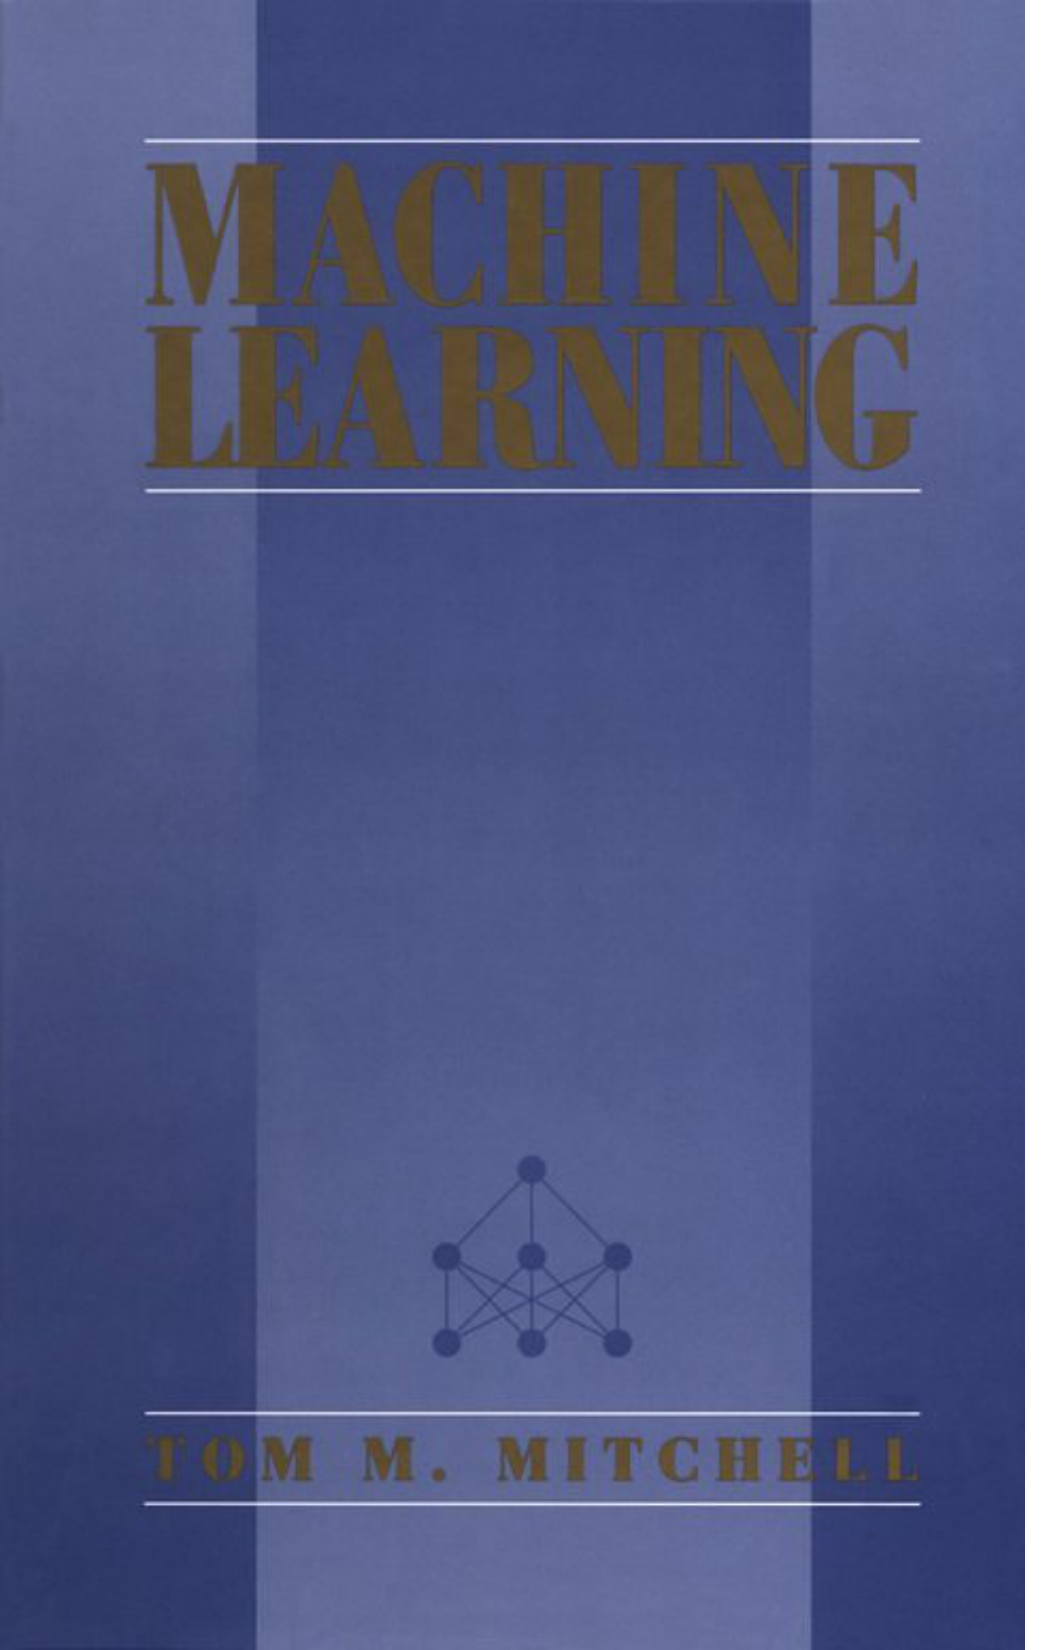
\includegraphics[width=0.9\linewidth]{figures/p1_b0.png}
\end{figure}

% --- page 2 ---
\subsection{Machine Learning}

Tom M. Mitchell

Chi tiết sản phẩm

• Bìa cứng: 432 trang ; Kích thước (tính bằng inch): 0,75 x 10,00 x 6,50

• Nhà xuất bản: McGraw-Hill Khoa học/Kỹ thuật/Toán học; (ngày 1 tháng 3 năm 1997)

• ISBN: 0070428077

• Đánh giá trung bình của khách hàng:

% missing image p2_b12
% missing image p2_b13
% missing image p2_b14
% missing image p2_b15
% missing image p2_b16
% missing image p2_b17
% missing image p2_b18
% missing image p2_b19
% missing image p2_b20
% missing image p2_b21
% missing image p2_b22
% missing image p2_b23
% missing image p2_b24
% missing image p2_b25
% missing image p2_b26
% missing image p2_b27
% missing image p2_b28
% missing image p2_b29
% missing image p2_b30
% missing image p2_b31
% missing image p2_b32
% missing image p2_b33
% missing image p2_b34
% missing image p2_b35
% missing image p2_b36
% missing image p2_b37
% missing image p2_b38
% missing image p2_b39
% missing image p2_b40
% missing image p2_b41
% missing image p2_b42
% missing image p2_b43
% missing image p2_b44
% missing image p2_b45
% missing image p2_b46
% missing image p2_b47
% missing image p2_b48
% missing image p2_b49
% missing image p2_b50
% missing image p2_b51
% missing image p2_b52
% missing image p2_b53
Dựa trên 16 đánh giá

• Xếp hạng doanh số của Amazon.com: 42.816

• Phổ biến ở: Redmond, WA (\#17) , Ithaca, NY (\#9)

Nhận xét biên tập

Từ Book News, Inc. Văn bản giới thiệu về các phương pháp tiếp cận chính đối với machine learning và nghiên cứu các thuật toán máy tính tự động cải thiện thông qua kinh nghiệm. Giới thiệu các khái niệm cơ bản từ thống kê, trí tuệ nhân tạo, lý thuyết thông tin và các ngành khác khi có nhu cầu, với phạm vi cân bằng giữa lý thuyết và lab, đồng thời trình bày các thuật toán chính kèm theo minh họa về cách sử dụng chúng. Bao gồm các bài tập theo chương. Data sets trực tuyến và việc triển khai một số thuật toán có sẵn trên một trang Web. Không có nền tảng trước đây về trí tuệ nhân tạo hoặc thống kê được giả định. Dành cho sinh viên đại học và sau đại học nâng cao về khoa học máy tính, kỹ thuật, thống kê và khoa học xã hội cũng như các chuyên gia phần mềm. Sách Tin tức, Inc.®, Portland, OR

Thông tin Sách: Trình bày các thuật toán và lý thuyết chính hình thành nên cốt lõi của machine learning. Thảo luận các vấn đề lý thuyết như Hiệu suất học tập thay đổi như thế nào theo số lượng ví dụ training được trình bày? Và Thuật toán học nào phù hợp nhất cho các loại nhiệm vụ học tập khác nhau? DLC: Thuật toán máy tính.

Mô tả Sách: Cuốn sách này đề cập đến lĩnh vực machine learning, nghiên cứu về các thuật toán cho phép các chương trình máy tính tự động cải tiến thông qua trải nghiệm. Cuốn sách này nhằm hỗ trợ các khóa học sau đại học cấp cao và cấp cơ sở trong machine learning

% --- page 3 ---
\begin{figure}[ht]
\centering
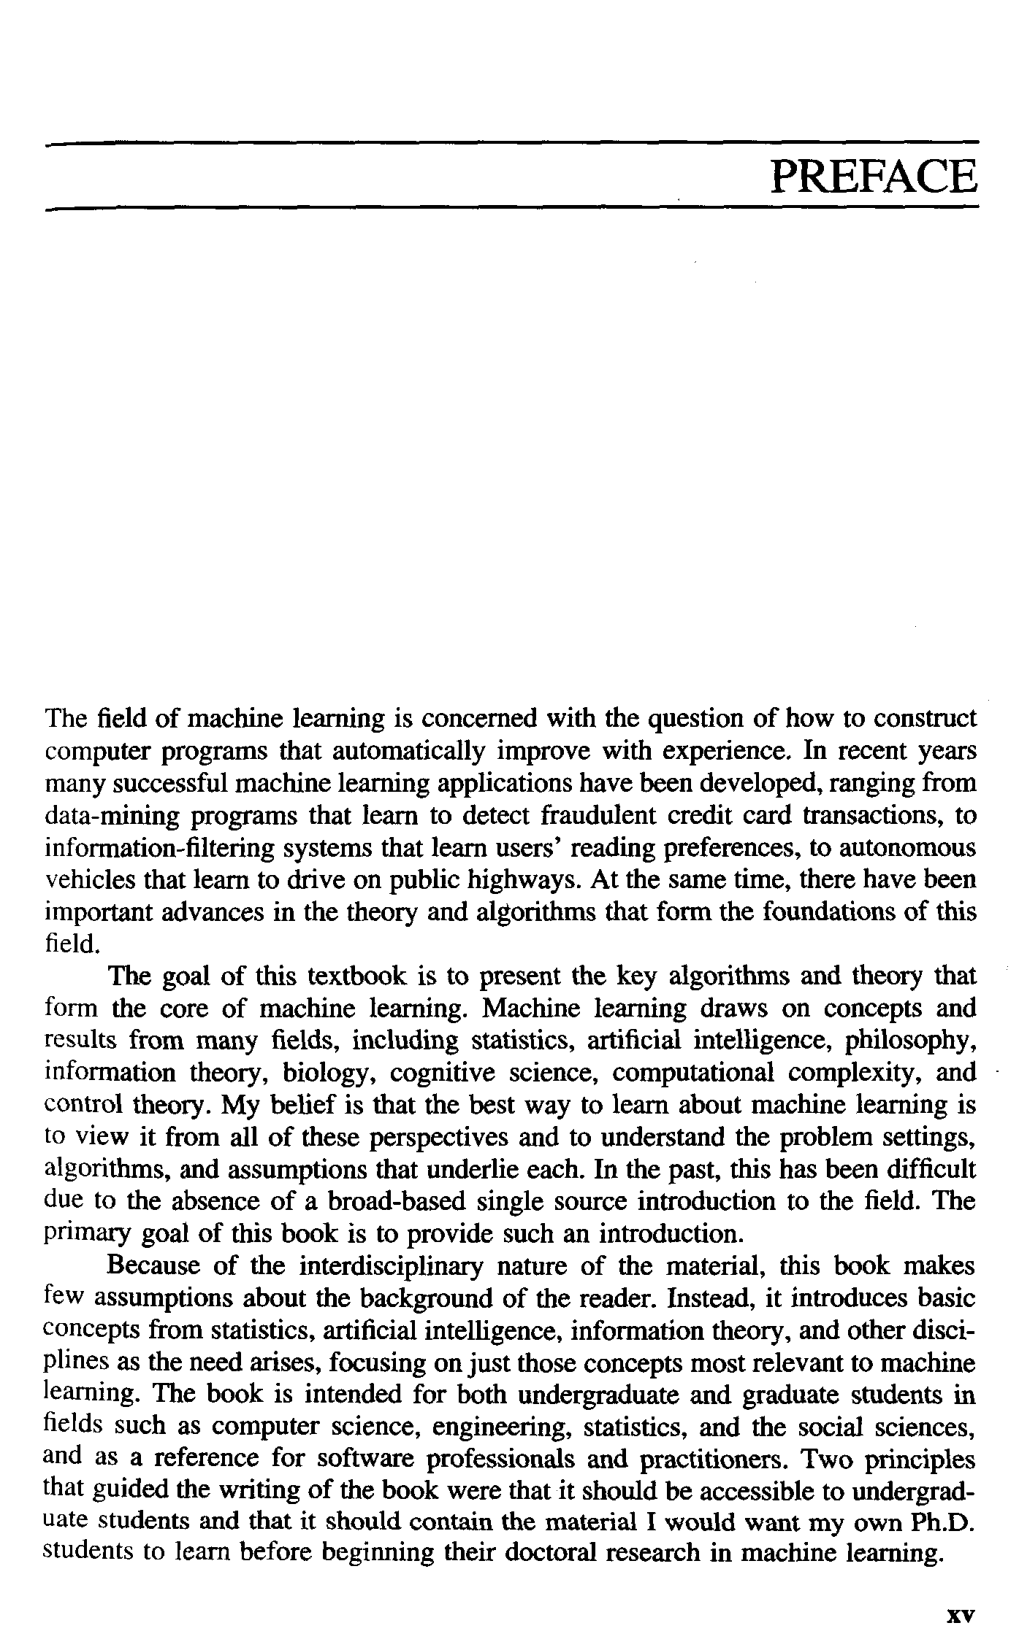
\includegraphics[width=0.9\linewidth]{figures/p3_b0.png}
\end{figure}

\section{PREFACE}

Lĩnh vực machine learning liên quan đến câu hỏi làm thế nào để xây dựng các chương trình máy tính có thể tự động cải thiện theo kinh nghiệm. Trong những năm gần đây, nhiều ứng dụng machine learning thành công đã được phát triển, từ các chương trình khai thác dữ liệu học cách phát hiện các giao dịch thẻ tín dụng gian lận, đến hệ thống lọc thông tin tìm hiểu sở thích đọc của người dùng, cho đến phương tiện tự hành học cách lái xe trên đường cao tốc công cộng. Đồng thời, đã có những tiến bộ quan trọng về lý thuyết và thuật toán hình thành nên nền tảng của lĩnh vực này.

Mục tiêu của cuốn sách giáo khoa này là trình bày các thuật toán và lý thuyết chính

Tạo thành cốt lõi của machine learning. Machine learning dựa trên các khái niệm và kết quả từ nhiều lĩnh vực, bao gồm thống kê, trí tuệ nhân tạo, triết học, lý thuyết thông tin, sinh học, khoa học nhận thức, độ phức tạp tính toán và lý thuyết điều khiển. Tôi tin rằng cách tốt nhất để tìm hiểu về machine learning là xem nó từ tất cả các khía cạnh này và hiểu các cài đặt vấn đề, thuật toán và giả định làm nền tảng cho từng khía cạnh. Trước đây, điều này gặp khó khăn do thiếu nguồn giới thiệu nguồn duy nhất trên diện rộng cho lĩnh vực này. Mục tiêu chính của cuốn sách này là cung cấp một lời giới thiệu như vậy.

Do tính chất liên ngành của tài liệu, cuốn sách này giúp

Vài giả định về hoàn cảnh của người đọc. Thay vào đó, nó giới thiệu cơ bản

Các khái niệm từ thống kê, trí tuệ nhân tạo, lý thuyết thông tin và các ngành khác khi có nhu cầu, chỉ tập trung vào những khái niệm phù hợp nhất với machine learning. Cuốn sách này dành cho cả sinh viên đại học và sau đại học trong các lĩnh vực như khoa học máy tính, kỹ thuật, thống kê và khoa học xã hội, đồng thời là tài liệu tham khảo cho các chuyên gia và người lab phần mềm. Hai nguyên tắc hướng dẫn việc viết cuốn sách là nó phải dễ tiếp cận đối với sinh viên đại học và nó phải chứa tài liệu mà tôi muốn có bằng Tiến sĩ của riêng mình. Sinh viên học trước khi bắt đầu nghiên cứu tiến sĩ về machine learning.

% --- page 4 ---
\subsection{Xvi PREFACE}

Nguyên tắc thứ ba hướng dẫn việc viết cuốn sách này là nó nên

Trình bày sự cân bằng giữa lý thuyết và lab. Lý thuyết Machine learning cố gắng trả lời các câu hỏi như "Hiệu suất học tập thay đổi như thế nào tùy theo số lượng ví dụ training được trình bày?" và "Thuật toán học tập nào phù hợp nhất cho các loại nhiệm vụ học tập khác nhau?" Cuốn sách này bao gồm các cuộc thảo luận về những vấn đề này và các vấn đề lý thuyết khác, dựa trên các cấu trúc lý thuyết từ thống kê,

Độ phức tạp giả định và phân tích Bayes. Việc lab machine learning được trình bày bằng cách trình bày các thuật toán chính trong lĩnh vực này, cùng với các dấu vết minh họa về hoạt động của chúng. Data sets trực tuyến và việc triển khai một số thuật toán có sẵn trên World Wide Web tại http://www.cs.cmu.edu/-tom1 mlbook.html. Chúng bao gồm mã và dữ liệu neural network để nhận dạng khuôn mặt, decision tree learning, mã và dữ liệu để phân tích khoản vay tài chính và lớp Bayes.

Mã sifier và dữ liệu để phân tích tài liệu văn bản. Tôi biết ơn một số đồng nghiệp đã giúp tạo ra những tài nguyên trực tuyến này, bao gồm Jason Rennie, Paul Hsiung, Jeff Shufelt, Matt Glickman, Scott Davies, Joseph O'Sullivan, Ken Lang, Andrew McCallum và Thorsten Joachims.

\subsection{ACKNOWLEDGMENTS}

Khi viết cuốn sách này, tôi may mắn được hỗ trợ bởi các chuyên gia kỹ thuật trong nhiều phân ngành tạo nên lĩnh vực machine learning. Cuốn sách này không thể được viết nếu không có sự giúp đỡ của họ. Tôi vô cùng biết ơn các nhà khoa học sau đây, những người đã dành thời gian xem xét bản thảo chương và, trong nhiều trường hợp, đã hướng dẫn tôi và giúp tổ chức các chương trong lĩnh vực chuyên môn riêng của họ.

Avrim Blum, Jaime Carbonell, William Cohen, Greg Cooper, Mark Craven, Ken DeJong, Jerry DeJong, Tom Dietterich, Susan Epstein, Oren Etzioni, Scott Fahlman, Stephanie Forrest, David Haussler, Haym Hirsh, Rob Holte,

Leslie Pack Kaelbling, Dennis Kibler, Moshe Koppel, John Koza, Miroslav

Kubat, John Lafferty, Ramon Lopez de Mantaras, Sridhar Mahadevan, Stan

Matwin, Andrew McCallum, Raymond Mooney, Andrew Moore, Katharina Morik, Steve Muggleton, Michael Pazzani, David Poole, Armand Prieditis, Jim Reggia, Stuart Russell, Lorenza Saitta, Claude Sammut, Jeff Schneider, Jude Shavlik, Devika Subramanian, Michael Swain, Gheorgh Tecuci, Sebastian Thrun, Peter Turney, Paul Utgoff, Manuela Veloso, Alex Waibel,

Stefan Wrobel và Yiming Yang.

Tôi cũng xin gửi lời cảm ơn tới nhiều giảng viên và sinh viên ở nhiều trường đại học khác nhau.

Những người đã thử nghiệm nhiều bản thảo khác nhau của cuốn sách này và đã đóng góp những đề xuất của mình. Mặc dù không có chỗ nào để cảm ơn hàng trăm sinh viên, người hướng dẫn và những người khác đã thử nghiệm các bản thảo trước đó của cuốn sách này, nhưng tôi muốn cảm ơn những người sau đây vì những nhận xét và thảo luận đặc biệt hữu ích:

Shumeet Baluja, Andrew Banas, Andy Barto, Jim Blackson, Justin Boyan, Rich Caruana, Philip Chan, Jonathan Cheyer, Lonnie Chrisman, Dayne Freitag, Geoff Gordon, Warren Greiff, Alexander Harm, Tom Ioerger, Thorsten

% --- page 5 ---
\begin{figure}[ht]
\centering

\includegraphics[width=0.9\linewidth]{figures/p5_b0.png}
\end{figure}

\subsection{PREFACE xvii}

Joachim, Atsushi Kawamura, Martina Klose, Sven Koenig, Jay Modi, Andrew Ng, Joseph O'Sullivan, Patrawadee Prasangsit, Doina Precup, Bob Price, Choon Quek, Sean Slattery, Belinda Thom, Astro Teller, Will Tracz

Tôi xin cảm ơn Joan Mitchell vì đã tạo mục lục cho cuốn sách. TÔI

Cũng xin gửi lời cảm ơn đến Jean Harpley vì đã giúp chỉnh sửa nhiều số liệu. Jane Loftus từ ETP Harrison đã cải thiện đáng kể cách trình bày thông qua việc sao chép bản thảo của cô ấy và nói chung đã giúp đưa bản thảo vượt qua những phức tạp của quá trình sản xuất cuối cùng. Eric Munson, biên tập viên của tôi tại McGraw Hill, đã khuyến khích và đưa ra kiến ​​thức chuyên môn trong tất cả các giai đoạn của dự án này.

Như mọi khi, món nợ lớn nhất mà một người mắc phải là đồng nghiệp, bạn bè và

Gia đình. Trong trường hợp của tôi, khoản nợ này đặc biệt lớn. Tôi khó có thể tưởng tượng ra một môi trường kích thích trí tuệ và có nhiều bạn bè hỗ trợ hơn những người tôi có ở Carnegie Mellon. Trong số những người đã giúp đỡ ở đây, tôi đặc biệt muốn cảm ơn Sebastian Thrun, người trong suốt dự án này luôn là nguồn động viên, chuyên môn kỹ thuật và hỗ trợ dưới mọi hình thức. Bố mẹ tôi, như mọi khi, động viên và hỏi “Xong chưa con?” vào đúng thời điểm. Cuối cùng, tôi phải cảm ơn gia đình mình: Meghan, Shannon và Joan. Họ chịu trách nhiệm về cuốn sách này theo nhiều cách hơn chính họ biết. Cuốn sách này được dành riêng cho họ.

Tom M. Mitchell

% --- page 6 ---
% --- page 7 ---
% --- page 8 ---
% --- page 9 ---
% --- page 10 ---
% --- page 11 ---
% --- page 12 ---
% --- page 13 ---
\subsection{CHAPTER}

\section{INTRODUCTION}

Kể từ khi máy tính được phát minh, chúng ta đã tự hỏi liệu chúng có thể được tạo ra để học hay không. Nếu chúng ta có thể hiểu cách lập trình cho chúng học-để cải thiện

Tự động bằng kinh nghiệm - tác động sẽ rất lớn. Hãy tưởng tượng máy tính-

Những người học từ hồ sơ y tế phương pháp điều trị nào hiệu quả nhất đối với những căn bệnh mới, những ngôi nhà học hỏi kinh nghiệm để tối ưu hóa chi phí năng lượng dựa trên cách sử dụng cụ thể của người cư ngụ hoặc trợ lý phần mềm cá nhân tìm hiểu sở thích ngày càng tăng của người dùng để làm nổi bật những câu chuyện đặc biệt có liên quan từ tờ báo buổi sáng trực tuyến. Sự hiểu biết thành công về cách làm cho máy tính học hỏi sẽ mở ra nhiều cách sử dụng máy tính mới và các cấp độ mới

Về năng lực và khả năng tùy biến. Và sự hiểu biết chi tiết về các thuật toán xử lý thông tin cho machine learning cũng có thể giúp hiểu rõ hơn về khả năng học tập (và khuyết tật) của con người.

Chúng ta vẫn chưa biết cách làm cho máy tính học gần như con người

Học hỏi. Tuy nhiên, các thuật toán đã được phát minh có hiệu quả đối với một số loại nhiệm vụ học tập nhất định và sự hiểu biết mang tính lý thuyết về việc học đang bắt đầu xuất hiện. Nhiều chương trình máy tính thực tế đã được phát triển để thể hiện các kiểu học tập hữu ích và các ứng dụng thương mại quan trọng đã bắt đầu xuất hiện. Đối với các vấn đề như nhận dạng giọng nói, các thuật toán dựa trên machine learning vượt trội hơn tất cả các phương pháp tiếp cận khác đã được thử nghiệm cho đến nay. Trong lĩnh vực được gọi là khai thác dữ liệu, thuật toán machine learning đang được sử dụng thường xuyên để khám phá kiến ​​thức có giá trị từ cơ sở dữ liệu thương mại lớn chứa hồ sơ bảo trì thiết bị, đơn xin vay vốn, giao dịch tài chính, hồ sơ y tế, v.v. Khi sự hiểu biết của chúng ta về máy tính tiếp tục phát triển, nó

% --- page 14 ---
\section{MACHINE LEARNING}

Dường như không thể tránh khỏi việc machine learning sẽ đóng vai trò ngày càng trung tâm trong khoa học máy tính và công nghệ máy tính.

Một vài thành tựu cụ thể cung cấp một cái nhìn thoáng qua về công nghệ tiên tiến:

Gram đã được phát triển để học cách nhận biết lời nói một cách thành công (Waibel 1989; Lee 1989), dự đoán tỷ lệ phục hồi của bệnh nhân viêm phổi (Cooper và cộng sự 1997), phát hiện việc sử dụng gian lận thẻ tín dụng, lái xe tự hành trên đường cao tốc công cộng (Pomerleau 1989), và chơi các trò chơi như cờ thỏ cáo ở cấp độ gần bằng thành tích của các nhà vô địch thế giới loài người (Tesauro 1992,

1995). Các kết quả lý thuyết đã được phát triển nhằm mô tả các đặc điểm cơ bản

Mối quan hệ giữa số lượng ví dụ training được quan sát, số lượng giả thuyết đang được xem xét và sai số dự kiến ​​trong các giả thuyết đã học. Chúng ta đang bắt đầu có được models ban đầu về khả năng học tập của con người và động vật cũng như để hiểu mối quan hệ của chúng với các thuật toán học tập được phát triển cho máy tính (ví dụ: Laird và cộng sự 1986; Anderson 1991; Qin và cộng sự 1992; Chi và Bassock 1989; Ahn và Brewer 1993). Trong các ứng dụng, thuật toán, lý thuyết và nghiên cứu về hệ thống sinh học, tốc độ tiến bộ đã tăng lên đáng kể trong thập kỷ qua. Một số ứng dụng gần đây của machine learning được tóm tắt trong Bảng 1.1. Langley và Simon (1995) và Rumelhart và cộng sự. (1994) khảo sát các ứng dụng bổ sung của machine learning.

Cuốn sách này trình bày lĩnh vực machine learning, mô tả nhiều loại

Model học tập, thuật toán, kết quả lý thuyết và ứng dụng. Machine learning vốn là một lĩnh vực đa ngành. Nó dựa trên kết quả từ trí tuệ nhân tạo, xác suất và thống kê, lý thuyết độ phức tạp tính toán, lý thuyết điều khiển, lý thuyết thông tin, triết học, tâm lý học, sinh học thần kinh và các lĩnh vực khác. Bảng 1.2 tóm tắt các ý tưởng chính từ mỗi lĩnh vực này có tác động đến lĩnh vực machine learning. Mặc dù tài liệu trong cuốn sách này dựa trên kết quả từ nhiều lĩnh vực khác nhau nhưng người đọc không cần phải là chuyên gia trong bất kỳ lĩnh vực nào trong số đó. Các ý tưởng chính được trình bày từ các lĩnh vực này bằng cách sử dụng vốn từ vựng của người không chuyên, với các thuật ngữ và khái niệm xa lạ được giới thiệu khi có nhu cầu.

\subsection{WELL-POSED LEARNING PROBLEMS}

Chúng ta hãy bắt đầu nghiên cứu về machine learning bằng cách xem xét một số nhiệm vụ học tập. Vì mục đích của cuốn sách này, chúng ta sẽ định nghĩa việc học một cách rộng rãi, bao gồm bất kỳ chương trình .computer nào giúp cải thiện hiệu suất của nó trong một số nhiệm vụ thông qua kinh nghiệm. Nói chính xác hơn,

Định nghĩa: Một chương trình máy tính được cho là học từ kinh nghiệm E với sự tôn trọng

Đối với một số loại nhiệm vụ T và thước đo hiệu suất P, nếu hiệu suất của nó ở các nhiệm vụ trong

T, được đo bằng P, cải thiện theo kinh nghiệm E.

Ví dụ: một chương trình máy tính học chơi checkers có thể cải thiện

Hiệu suất của nó được đo bằng khả năng giành chiến thắng ở loại nhiệm vụ liên quan đến

Chơi các trò chơi checkers, thông qua kinh nghiệm có được khi chơi trò chơi với

Chính nó. Nói chung, để có một vấn đề học tập được xác định rõ ràng, chúng ta phải xác định những

% --- page 15 ---
\subsection{CHAPTER 1 INTRODUCITON 3}

\section{Học cách nhận biết lời nói.}

Tất cả các hệ thống nhận dạng giọng nói thành công nhất đều sử dụng machine learning dưới một số hình thức. Ví dụ: hệ thống SPHINX (ví dụ: Lee 1989) học các chiến lược dành riêng cho người nói để nhận biết các âm thanh nguyên thủy (âm vị) và các từ từ tín hiệu giọng nói được quan sát. Các phương pháp Neural network learning (ví dụ, Waibel và cộng sự 1989) và các phương pháp học ẩn Markov models (ví dụ, Lee 1989) có hiệu quả trong việc tự động tùy chỉnh theo từng loa, từ vựng, đặc điểm micrô, tiếng ồn nền, v.v. Các kỹ thuật tương tự có ứng dụng tiềm năng trong nhiều vấn đề giải thích tín hiệu.

\section{Học lái xe tự lái.}

Các phương pháp Machine learning đã được sử dụng để training các phương tiện được điều khiển bằng máy tính cách lái chính xác khi lái xe trên nhiều loại đường khác nhau. Ví dụ, hệ thống ALVINN (Pomerleau 1989) đã sử dụng các chiến lược đã học được của mình để lái xe không có trợ lực ở tốc độ 70 dặm một giờ trong 90 dặm trên đường cao tốc công cộng cùng với các loại xe khác. Các kỹ thuật tương tự có thể ứng dụng được trong nhiều bài toán điều khiển dựa trên cảm biến.

\section{Học cách classification các cấu trúc thiên văn mới.}

Các phương pháp Machine learning đã được áp dụng cho nhiều cơ sở dữ liệu lớn khác nhau để tìm hiểu các quy luật chung tiềm ẩn trong dữ liệu. Ví dụ: thuật toán decision tree learning đã được NASA sử dụng để tìm hiểu cách classification các thiên thể từ Khảo sát bầu trời của đài quan sát Palomar lần thứ hai (Fayyad và cộng sự 1995). Hệ thống này hiện được sử dụng để tự động classification tất cả các vật thể trong Khảo sát bầu trời, bao gồm ba terrabyte dữ liệu hình ảnh.

\section{Học chơi cờ thỏ cáo đẳng cấp thế giới.}

Các chương trình máy tính thành công nhất để chơi trò chơi như cờ thỏ cáo đều dựa trên thuật toán học máy. Ví dụ, chương trình máy tính hàng đầu thế giới dành cho cờ thỏ cáo, TD-GAMMON (Tesauro 1992, 1995). Đã học được chiến lược của nó bằng cách chơi hơn một triệu trận đấu tập với chính nó. Bây giờ nó chơi ở cấp độ cạnh tranh với nhà vô địch thế giới loài người. Các kỹ thuật tương tự có ứng dụng trong nhiều bài toán thực tế trong đó không gian tìm kiếm rất lớn phải được kiểm tra một cách hiệu quả.

\noindent\textit{TABLE 1.1 Một số ứng dụng thành công của học máy.}

Ba features: loại nhiệm vụ, thước đo hiệu suất cần cải thiện và nguồn kinh nghiệm.

Một vấn đề học tập checkers:

\subsection{Nhiệm vụ T: chơi checkers}

\section{Thước đo hiệu suất P: phần trăm số trận thắng trước đối thủ}

\subsection{Kinh nghiệm training E: chơi trò luyện tập với chính nó}

Chúng ta có thể xác định nhiều vấn đề học tập theo cách này, chẳng hạn như học tập

Để nhận dạng các từ viết tay hoặc học lái ô tô robot tự động.

Một bài toán học nhận dạng chữ viết tay:

\section{Nhiệm vụ T: nhận biết và classification chữ viết tay trong ảnh}

\section{Thước đo hiệu suất P: phần trăm số từ được phân loại chính xác}

% --- page 16 ---
\section{MACHINE LEARNING}

Trí tuệ nhân tạo Học cách biểu diễn các khái niệm mang tính biểu tượng. Machine learning là một vấn đề tìm kiếm. Học tập như một cách tiếp cận để cải thiện việc giải quyết vấn đề. Sử dụng kiến ​​thức có sẵn cùng với dữ liệu training để hướng dẫn việc học.

\section{phương pháp Bayes}

Định lý Bayes làm cơ sở tính xác suất của các giả thuyết. Classifier naive Bayes. Các thuật toán ước tính giá trị của các biến không quan sát được.

\section{Lý thuyết độ phức tạp tính toán}

Giới hạn lý thuyết về độ phức tạp vốn có của các nhiệm vụ học tập khác nhau, được đo lường bằng nỗ lực tính toán, số lượng ví dụ training, số lỗi, v.v. Cần có để học. Lý thuyết điều khiển Các quy trình học cách kiểm soát các quy trình nhằm tối ưu hóa các mục tiêu được xác định trước và học cách dự đoán trạng thái tiếp theo của quy trình mà chúng đang kiểm soát.

\section{Lý thuyết thông tin}

Các phép đo entropy và nội dung thông tin. Các phương pháp tiếp cận có độ dài mô tả tối thiểu đối với việc học. Mã tối ưu và mối quan hệ của chúng với trình tự training tối ưu để mã hóa giả thuyết. Triết học Con dao cạo của Occam, gợi ý rằng giả thuyết đơn giản nhất là tốt nhất. Phân tích sự biện minh cho việc khái quát hóa ngoài dữ liệu được quan sát.

\section{Tâm lý học và sinh học thần kinh}

Quy luật lũy thừa của thực tiễn, trong đó phát biểu rằng trong một phạm vi rất rộng các vấn đề học tập, thời gian response của mọi người sẽ cải thiện khi lab theo quy luật lũy thừa. Các nghiên cứu sinh học thần kinh thúc đẩy việc học tập neural network models nhân tạo.

\section{Thống kê}

Đặc điểm của các lỗi (ví dụ: bias và variance) xảy ra khi ước tính độ chính xác của giả thuyết dựa trên một mẫu dữ liệu hạn chế. Khoảng tin cậy, kiểm định thống kê.

\noindent\textit{TABLE 1.2 Một số nguyên tắc và ví dụ về ảnh hưởng của chúng đối với machine learning.}

\section{Kinh nghiệm training E: cơ sở dữ liệu các từ viết tay với các classification nhất định}

\subsection{Hư cấu}

Một bài toán học lái xe robot:

\section{Nhiệm vụ T: lái xe trên đường cao tốc bốn làn công cộng sử dụng cảm biến thị giác}

\section{Thước đo hiệu suất P: khoảng cách trung bình đã di chuyển trước khi xảy ra lỗi (được đánh giá}

\subsection{Bởi người giám sát con người)}

\section{Kinh nghiệm training E: chuỗi hình ảnh và ghi lại lệnh lái-}

\subsection{Ed trong khi quan sát người lái xe}

Định nghĩa của chúng ta về học tập đủ rộng để bao gồm hầu hết các nhiệm vụ mà chúng ta

Thường gọi là nhiệm vụ "học tập", khi chúng ta sử dụng từ này trong ngôn ngữ hàng ngày. Nó cũng đủ rộng để bao gồm các chương trình máy tính cải thiện trải nghiệm theo những cách khá đơn giản. Ví dụ, hệ thống cơ sở dữ liệu

% --- page 17 ---
\subsection{CHAFTlB 1 INTRODUCTION 5}

Cho phép người dùng cập nhật các mục nhập dữ liệu sẽ phù hợp với định nghĩa của chúng ta về hệ thống học tập: nó cải thiện hiệu suất của nó trong việc trả lời các truy vấn cơ sở dữ liệu, dựa trên kinh nghiệm thu được từ các bản cập nhật cơ sở dữ liệu. Thay vì lo lắng về việc liệu loại hoạt động này có thuộc ý nghĩa đàm thoại thân mật thông thường của từ “học tập” hay không, chúng ta sẽ đơn giản áp dụng định nghĩa kỹ thuật của mình về loại chương trình được cải thiện thông qua trải nghiệm. Trong lớp này, chúng ta sẽ tìm thấy nhiều loại vấn đề đòi hỏi các giải pháp ít nhiều phức tạp. Mối quan tâm của chúng ta ở đây không phải là phân tích ý nghĩa của từ “học tập” trong tiếng Anh như nó được sử dụng trong ngôn ngữ hàng ngày. Thay vào đó, mục tiêu của chúng ta là xác định chính xác một lớp vấn đề bao gồm các hình thức học tập thú vị, khám phá các thuật toán giải quyết các vấn đề đó và hiểu cấu trúc cơ bản của các vấn đề và quy trình học tập.

\subsection{DESIGNING A LEARNING SYSTEM}

Để minh họa một số vấn đề thiết kế cơ bản và cách tiếp cận machine learning, chúng ta hãy xem xét việc thiết kế một chương trình học cách chơi checkers, với mục tiêu đưa nó tham gia giải đấu checkers thế giới. Chúng ta áp dụng thước đo hiệu suất rõ ràng: phần trăm số trận thắng trong giải đấu thế giới này.

\subsubsection{Lựa chọn kinh nghiệm training}

Lựa chọn thiết kế đầu tiên mà chúng ta phải đối mặt là chọn loại trải nghiệm training mà hệ thống của chúng ta sẽ học hỏi. Loại kinh nghiệm training sẵn có có thể có tác động đáng kể đến sự thành công hay thất bại của người học. Một thuộc tính quan trọng là liệu trải nghiệm training có cung cấp response trực tiếp hay gián tiếp về các lựa chọn do hệ thống thực hiện đưa ra hay không. Ví dụ: khi học chơi checkers,

Hệ thống có thể học từ các ví dụ training trực tiếp bao gồm checkers riêng lẻ

Các trạng thái bàn cờ và nước đi đúng cho từng trạng thái. Ngoài ra, nó có thể chỉ có thông tin gián tiếp bao gồm trình tự di chuyển và outcomes cuối cùng của các trò chơi khác nhau đã chơi. Trong trường hợp sau này, thông tin về tính chính xác của các nước đi cụ thể ở đầu trò chơi phải được suy ra một cách gián tiếp từ thực tế là cuối cùng trò chơi đã thắng hoặc thua. Ở đây, người học phải đối mặt với một vấn đề bổ sung về việc ấn định công trạng hoặc xác định mức độ mà mỗi nước đi trong chuỗi xứng đáng được công nhận hoặc đổ lỗi cho outcome cuối cùng. Việc phân công công lao có thể là một vấn đề đặc biệt khó khăn vì trò chơi có thể bị thua ngay cả khi những bước đi đầu tiên là tối ưu, nếu sau đó là những bước đi kém. Do đó, học từ response training trực tiếp thường dễ hơn học từ response gián tiếp.

Thuộc tính quan trọng thứ hai của kinh nghiệm training là mức độ mà

Người học kiểm soát trình tự của các ví dụ training. Ví dụ, người học có thể dựa vào giáo viên để chọn các trạng thái bảng thông tin và đưa ra nước đi chính xác cho từng trạng thái. Ngoài ra, người học có thể tự mình đề xuất các trạng thái trên bảng mà họ cảm thấy đặc biệt khó hiểu và yêu cầu giáo viên thực hiện động tác chính xác. Hoặc người học có thể có toàn quyền kiểm soát cả trạng thái bảng và classification training (gián tiếp), giống như khi học bằng cách chơi với chính mình mà không có giáo viên.

% --- page 18 ---
Hiện tại. Lưu ý trong trường hợp cuối cùng này, người học có thể chọn giữa việc thử nghiệm các trạng thái bảng mới mà họ chưa xem xét hoặc trau dồi kỹ năng của mình bằng cách chơi các biến thể nhỏ của các lối chơi mà hiện tại họ thấy có triển vọng nhất. Các chương tiếp theo xem xét một số cài đặt cho việc học, bao gồm cài đặt trong đó trải nghiệm training được cung cấp bởi một quy trình ngẫu nhiên ngoài tầm kiểm soát của người học, cài đặt trong đó người học có thể đặt ra nhiều loại truy vấn khác nhau cho giáo viên chuyên gia và cài đặt trong đó người học thu thập các ví dụ training bằng cách tự động khám phá môi trường của nó.

Thuộc tính quan trọng thứ ba của trải nghiệm training là nó thể hiện tốt như thế nào.

Gửi phân phối các mẫu mà qua đó hiệu suất hệ thống cuối cùng P phải được đo lường. Nói chung, việc học là đáng tin cậy nhất khi các mẫu training tuân theo sự phân bố tương tự như các mẫu thử nghiệm trong tương lai. Trong kịch bản học tập checkers của chúng ta, chỉ số hiệu suất P là phần trăm số trò chơi mà hệ thống thắng trong giải đấu thế giới. Nếu kinh nghiệm training E của nó chỉ bao gồm các trò chơi được chơi với chính nó, thì có một nguy cơ rõ ràng là kinh nghiệm training này có thể không đại diện đầy đủ cho sự phân bổ các tình huống mà nó sẽ được kiểm tra sau này. Ví dụ: người học có thể không bao giờ gặp phải một số trạng thái bàn cờ quan trọng nhất định mà rất có thể do nhà vô địch checkers của con người chơi. Trong thực tế, thường cần phải học hỏi từ việc phân phối các ví dụ hơi khác so với những ví dụ mà hệ thống cuối cùng sẽ được đánh giá (ví dụ: nhà vô địch checkers thế giới có thể không quan tâm đến việc giảng dạy chương trình!). Những tình huống như vậy là có vấn đề vì việc thành thạo một phân phối mẫu sẽ không cần thiết dẫn đến hiệu suất cao so với một số phân phối khác. Chúng ta sẽ thấy rằng hầu hết lý thuyết hiện tại về machine learning đều dựa trên giả định quan trọng rằng việc phân phối các mẫu training giống hệt với việc phân phối các mẫu thử nghiệm. Mặc dù chúng ta cần phải đưa ra giả định này để đạt được các kết quả lý thuyết, nhưng điều quan trọng cần ghi nhớ là giả định này thường bị vi phạm trong thực tế.

Để tiếp tục thiết kế, chúng ta hãy quyết định rằng hệ thống của chúng ta sẽ training bằng cách

Chơi trò chơi chống lại chính nó. Điều này có ưu điểm là không cần có training viên bên ngoài và do đó nó cho phép hệ thống tạo ra nhiều dữ liệu training khi thời gian cho phép. Bây giờ chúng ta có một nhiệm vụ học tập được chỉ định đầy đủ.

Một vấn đề học tập checkers:

\section{Nhiệm vụ T: chơi checkers}

\section{Thước đo thành tích P: phần trăm số trận thắng trong giải đấu thế giới}

\section{Kinh nghiệm training E: trận đấu với chính nó}

Để hoàn thiện việc thiết kế hệ thống học tập, bây giờ chúng ta phải chọn

1. Loại kiến ​​thức chính xác cần học

2. Sự thể hiện kiến ​​thức mục tiêu này 3. Cơ chế học tập

% --- page 19 ---
\section{CHAFTER tôi INTRODUCTION 7}

\subsubsection{Chọn hàm mục tiêu}

Lựa chọn thiết kế tiếp theo là xác định chính xác loại kiến ​​thức nào sẽ được học và cách thức sử dụng kiến ​​thức đó trong chương trình biểu diễn. Chúng ta hãy bắt đầu với chương trình chơi checkers có thể tạo ra các nước đi hợp pháp từ bất kỳ trạng thái bàn cờ nào. Chương trình chỉ cần học cách chọn nước đi tốt nhất trong số những nước đi hợp pháp này. Nhiệm vụ học tập này đại diện cho một lớp lớn các nhiệm vụ trong đó các bước đi hợp pháp nhằm xác định một không gian tìm kiếm lớn nào đó đã được biết đến một cách tiên nghiệm nhưng chiến lược tìm kiếm tốt nhất lại không được biết đến. Nhiều vấn đề tối ưu hóa thuộc loại này, chẳng hạn như các vấn đề về lập kế hoạch và kiểm soát các quy trình sản xuất trong đó các bước sản xuất có sẵn được hiểu rõ, nhưng chiến lược tốt nhất để sắp xếp chúng thì không.

Với bối cảnh này, chúng ta phải học cách lựa chọn trong số các động thái hợp pháp,

Sự lựa chọn rõ ràng nhất cho loại thông tin cần học là một chương trình hoặc chức năng chọn nước đi tốt nhất cho bất kỳ trạng thái bàn cờ nhất định nào. Chúng ta hãy gọi đây là

Chức năng ChooseMove và sử dụng ký hiệu ChooseMove : B -+ M để biểu thị

Rằng hàm này chấp nhận làm đầu vào cho bất kỳ bảng nào từ tập hợp các trạng thái bảng hợp lệ B và tạo ra đầu ra một số bước đi từ tập hợp các bước đi hợp lệ M. Trong suốt cuộc thảo luận về machine learning, chúng ta sẽ thấy hữu ích khi giảm vấn đề cải thiện hiệu suất P ở nhiệm vụ T thành vấn đề học một số hàm mục tiêu cụ thể như ChooseMove. Do đó, việc lựa chọn hàm mục tiêu sẽ là lựa chọn thiết kế quan trọng.

Mặc dù ChooseMove là một lựa chọn hiển nhiên cho hàm mục tiêu trong

Ví dụ: chức năng này sẽ rất khó học do loại trải nghiệm training gián tiếp có sẵn trong hệ thống của chúng ta. Một chức năng mục tiêu thay thế và một chức năng sẽ dễ học hơn trong cài đặt này là đánh giá

Hàm gán điểm số cho bất kỳ trạng thái bảng nhất định nào. Chúng ta hãy gọi hàm mục tiêu này là V và một lần nữa sử dụng ký hiệu V : B + 8 để biểu thị rằng V ánh xạ bất kỳ trạng thái bảng pháp lý nào từ tập B sang một giá trị thực nào đó (chúng ta sử dụng 8 để biểu thị tập hợp số thực). Chúng ta dự định chức năng mục tiêu V này sẽ gán điểm cao hơn cho các trạng thái bảng tốt hơn. Nếu hệ thống có thể học thành công hàm mục tiêu V như vậy thì nó có thể dễ dàng sử dụng hàm đó để chọn nước đi tốt nhất từ ​​bất kỳ vị trí hiện tại nào trên bàn cờ. Điều này có thể được thực hiện bằng cách tạo ra trạng thái bảng kế tiếp được tạo ra bởi mỗi nước đi hợp lệ, sau đó sử dụng V để chọn trạng thái kế tiếp tốt nhất và do đó là nước đi hợp pháp tốt nhất.

Giá trị chính xác của hàm mục tiêu V đối với bất kỳ giá trị nào đã cho là bao nhiêu?

Trạng thái hội đồng quản trị? Tất nhiên, bất kỳ chức năng đánh giá nào gán điểm cao hơn cho trạng thái bảng tốt hơn đều có tác dụng. Tuy nhiên, chúng ta sẽ thấy hữu ích khi xác định một hàm mục tiêu V cụ thể trong số nhiều hàm tạo ra cách chơi tối ưu. Như chúng ta sẽ thấy, điều này sẽ làm cho việc thiết kế thuật toán training trở nên dễ dàng hơn. Do đó, chúng ta hãy xác định giá trị đích V(b) cho trạng thái bảng tùy ý b trong B, như sau:

1. Nếu b là trạng thái ván cuối cùng thắng thì V(b) = 100 2. Nếu b là trạng thái ván cuối cùng thua thì V ( b ) = -100 3. Nếu b là trạng thái ván cuối cùng hòa thì V ( b ) = 0

% --- page 20 ---
4. Nếu b không phải là trạng thái cuối cùng của trò chơi thì V(b) = V(bl), trong đó b' là trạng thái tốt nhất

Trạng thái bàn cuối cùng có thể đạt được bắt đầu từ b và chơi tối ưu cho đến cuối trò chơi (giả sử đối thủ cũng chơi tối ưu).

Trong khi định nghĩa đệ quy này chỉ định giá trị V(b) cho mỗi bảng

Trạng thái b, định nghĩa này không thể sử dụng được bởi trình phát checkers của chúng ta vì nó không thể tính toán một cách hiệu quả. Ngoại trừ các trường hợp tầm thường (trường hợp 1-3) trong đó trò chơi đã kết thúc, việc xác định giá trị của V(b) cho một trạng thái bàn cờ cụ thể yêu cầu (trường hợp 4) tìm kiếm trước lối chơi tối ưu cho đến hết trò chơi! Vì định nghĩa này không thể tính toán một cách hiệu quả bằng chương trình chơi checkers của chúng ta nên chúng ta nói rằng đó là định nghĩa không hoạt động. Mục tiêu của việc học trong trường hợp này là khám phá mô tả hoạt động của V ; nghĩa là, một mô tả có thể được chương trình chơi checkers sử dụng để đánh giá các trạng thái và chọn nước đi trong giới hạn thời gian thực tế.

Vì vậy, chúng ta đã quy giản nhiệm vụ học tập trong trường hợp này thành vấn đề về

Khám phá một mô tả hoạt động của hàm mục tiêu lý tưởng V. Nói chung có thể rất khó để học một dạng hoạt động như vậy của V một cách hoàn hảo. Trong thực tế, chúng ta thường mong đợi các thuật toán học chỉ thu được một số xấp xỉ nào đó với hàm mục tiêu và vì lý do này, quá trình học hàm mục tiêu thường được gọi là xấp xỉ hàm. Trong cuộc thảo luận hiện tại, chúng ta sẽ sử dụng ký hiệu ? Để đề cập đến hàm mà chương trình của chúng ta thực sự học được, để phân biệt nó với hàm mục tiêu lý tưởng V.

\subsection{Chọn biểu diễn cho hàm đích}

Bây giờ chúng ta đã xác định được hàm mục tiêu lý tưởng V, chúng ta phải chọn một biểu diễn mà chương trình học sẽ sử dụng để mô tả hàm c mà nó sẽ học. Giống như các lựa chọn thiết kế trước đó, chúng ta lại có nhiều lựa chọn. Ví dụ, chúng ta có thể cho phép chương trình biểu diễn bằng cách sử dụng một bảng lớn với một

Mục nhập chỉ định giá trị cho từng trạng thái bảng riêng biệt. Hoặc chúng ta có thể cho phép nó thể hiện bằng cách sử dụng một tập hợp các quy tắc phù hợp với features của bảng

Trạng thái hoặc hàm đa thức bậc hai của bảng features được xác định trước hoặc neural network nhân tạo. Nói chung, sự lựa chọn đại diện này liên quan đến một sự đánh đổi quan trọng. Một mặt, chúng ta mong muốn chọn một biểu diễn có tính biểu cảm cao để cho phép biểu diễn gần đúng nhất có thể với hàm mục tiêu lý tưởng V. Mặt khác, biểu diễn càng biểu cảm thì chương trình sẽ càng yêu cầu nhiều dữ liệu training hơn để chọn trong số các giả thuyết thay thế mà nó có thể biểu diễn. Để thảo luận ngắn gọn, chúng ta hãy chọn một cách biểu diễn đơn giản: đối với bất kỳ trạng thái bảng nhất định nào, hàm c sẽ được tính dưới dạng tổ hợp tuyến tính của bảng features sau:

\section{xl: số quân đen trên bàn cờ}

\subsection{X\_2: số quân đỏ trên bàn cờ}

\section{xs: số quân đen trên bàn cờ}

\section{x\_4: số quân vua đỏ trên bàn cờ}

% --- page 21 ---
\section{CHAPTER tôi INTRODUCTION 9}

$X_{5}$: số quân đen bị quân đỏ đe dọa (tức là quân đỏ có thể bắt được ở lượt tiếp theo)

\subsection{X\_6: số quân đỏ bị quân đen đe dọa}

Do đó, chương trình học của chúng ta sẽ biểu diễn c(b) dưới dạng hàm tuyến tính của

\subsection{Hình thức}

Trong đó wo đến W6 là coefficients số hoặc weight được thuật toán học chọn. Các giá trị đã học cho các weight w l thông qua W6 sẽ xác định tầm quan trọng tương đối của các bảng features khác nhau trong việc xác định giá trị của bảng, trong khi weight wo sẽ cung cấp hằng số cộng cho giá trị bảng.

Để tóm tắt các lựa chọn thiết kế của chúng ta cho đến nay, chúng ta đã xây dựng bản gốc

Xây dựng vấn đề học tập bằng cách chọn loại kinh nghiệm training, hàm mục tiêu cần học và biểu diễn cho hàm mục tiêu này. Nhiệm vụ học tập phức tạp của chúng ta bây giờ là

Thiết kế một phần chương trình học checkers:

Nhiệm vụ T: chơi checkers Thước đo hiệu suất P: phần trăm số trận thắng trong giải đấu thế giới Kinh nghiệm training E: các trận đấu với chính nó

\subsection{Hàm mục tiêu: V:Board + 8 Biểu diễn hàm mục tiêu}

Ba mục đầu tiên ở trên tương ứng với đặc điểm kỹ thuật của nhiệm vụ học tập,

Trong khi hai mục cuối cùng tạo thành các lựa chọn thiết kế để thực hiện chương trình học tập. Lưu ý rằng hiệu quả thực sự của tập hợp các lựa chọn thiết kế này là giảm vấn đề học chiến lược checkers thành vấn đề học các giá trị cho coefficients từ w 6 trong biểu diễn hàm mục tiêu.

\subsubsection{Lựa chọn thuật toán xấp xỉ hàm}

Để tìm hiểu hàm mục tiêu f, chúng ta cần một tập hợp các ví dụ training, mỗi ví dụ mô tả một trạng thái bảng b cụ thể và giá trị training Vtrain(b) cho b. Nói cách khác, mỗi ví dụ training là một cặp có thứ tự có dạng (b, V',,,i,(b)). Vì

Ví dụ, ví dụ training sau đây mô tả trạng thái bàn cờ b trong đó quân đen đã thắng trò chơi (lưu ý $x_{2}$ = 0 chỉ ra rằng quân đỏ không còn quân nào) và do đó giá trị hàm mục tiêu VZrain(b) là +100.

% --- page 22 ---
\section{MACHINE LEARNING}

Dưới đây chúng ta mô tả một quy trình đầu tiên lấy các ví dụ training như vậy từ

Kinh nghiệm training gián tiếp có sẵn cho người học, sau đó điều chỉnh weight

Wi để phù hợp nhất với những ví dụ training này.

1.2.4.1 ESTIMATING TRAINING VALUES

Hãy nhớ lại rằng theo cách chúng ta xây dựng vấn đề học tập, thông tin training duy nhất có sẵn cho người học là liệu trò chơi cuối cùng thắng hay thua. Mặt khác, chúng ta yêu cầu các ví dụ training gán điểm cụ thể cho các trạng thái bảng cụ thể. Mặc dù có thể dễ dàng gán một giá trị cho các trạng thái bàn cờ tương ứng với thời điểm kết thúc trò chơi, nhưng cách gán giá trị training cho nhiều trạng thái bàn cờ trung gian hơn xảy ra trước khi trò chơi kết thúc lại ít rõ ràng hơn. Tất nhiên, việc trò chơi cuối cùng thắng hay thua không nhất thiết chỉ ra rằng mọi trạng thái bàn cờ dọc theo đường đi của trò chơi đều nhất thiết là tốt hay xấu. Ví dụ: ngay cả khi chương trình thua trò chơi, vẫn có thể xảy ra trường hợp trạng thái bàn cờ xảy ra sớm trong trò chơi phải được đánh giá rất cao và nguyên nhân dẫn đến thua là do nước đi kém tiếp theo.

Bất chấp sự mơ hồ cố hữu trong việc ước tính giá trị training cho học sinh trung cấp

Hội đồng quản trị cho biết, một cách tiếp cận đơn giản đã được chứng minh là thành công một cách đáng ngạc nhiên. Cách tiếp cận này là gán giá trị training của Krain(b) cho bất kỳ trạng thái bảng trung gian b nào là ?(\textasciitilde{}người kế nhiệm(b)), ở đâu ? Là giá trị gần đúng hiện tại của người học với

V và trong đó Người kế nhiệm(b) biểu thị trạng thái bảng tiếp theo theo sau b mà nó

Một lần nữa đến lượt chương trình đi (tức là trạng thái bàn cờ theo sau nước đi của chương trình và response của đối thủ). Quy tắc ước tính giá trị training này có thể được tóm tắt như sau:

\textasciitilde{} ul k để ước tính giá trị training.

V,,, tôi. (b) c c(\textasciitilde{}người kế nhiệm(b))

Mặc dù việc sử dụng phiên bản hiện tại của f để training estimate có vẻ lạ

Các giá trị sẽ được sử dụng để tinh chỉnh chức năng tương tự này, hãy lưu ý rằng chúng ta đang sử dụng estimates của giá trị của Successor(b) đến estimate giá trị của trạng thái bảng b. Bằng trực giác, chúng ta có thể thấy điều này sẽ hợp lý nếu ? Có xu hướng chính xác hơn đối với các trạng thái bàn cờ gần kết thúc trò chơi. Trên thực tế, trong một số điều kiện nhất định (được thảo luận trong Chương 13), cách tiếp cận ước tính lặp đi lặp lại các giá trị training dựa trên estimates của các giá trị trạng thái kế tiếp có thể được chứng minh là hội tụ về phía estimates hoàn hảo của Vtrain.

1.2.4.2 ADJUSTING THE WEIGHTS

Tất cả những gì còn lại là xác định thuật toán học để chọn các weight wi để\textasciicircum{} phù hợp nhất với tập ví dụ training \{(b, Vtrain(b))\}. Bước đầu tiên chúng ta phải xác định

Ý của chúng ta là phù hợp nhất với dữ liệu training. Một cách tiếp cận phổ biến là xác định giả thuyết hoặc tập hợp weight tốt nhất để giảm thiểu sai số bình phương E giữa các giá trị training và các giá trị được dự đoán bởi giả thuyết V.

% --- page 23 ---
Vì vậy, chúng ta tìm kiếm các weight, hay tương đương là c, để giảm thiểu E cho các ví dụ training được quan sát. Chương 6 thảo luận về các cài đặt trong đó việc giảm thiểu tổng sai số bình phương tương đương với việc tìm ra giả thuyết có khả năng xảy ra cao nhất dựa trên dữ liệu training được quan sát.

Một số thuật toán được biết đến để tìm weight của hàm tuyến tính

Giảm thiểu E được xác định theo cách này. Trong trường hợp của chúng ta, chúng ta yêu cầu một thuật toán sẽ tinh chỉnh dần các weight khi có sẵn các ví dụ training mới và thuật toán đó sẽ có khả năng ngăn ngừa lỗi trong các giá trị training ước tính này. Một thuật toán như vậy được gọi là bình phương trung bình nhỏ nhất hoặc quy tắc training LMS. Đối với mỗi mẫu training được quan sát, nó sẽ điều chỉnh weight một lượng nhỏ theo hướng giảm lỗi trên mẫu training này. Như đã thảo luận trong Chương 4, thuật toán này có thể được xem như thực hiện tìm kiếm giảm dần độ dốc ngẫu nhiên thông qua không gian của các giả thuyết có thể có (giá trị weight) để cực tiểu hóa enor bình phương E. Thuật toán LMS được định nghĩa như sau:

Quy tắc cập nhật trọng lượng LMS.

\subsection{Đối với mỗi ví dụ training (b, Kmin(b))}

Sử dụng các weight hiện tại để tính ?(b) Với mỗi weight mi, hãy cập nhật nó thành

Ở đây q là một hằng số nhỏ (ví dụ: 0,1) điều tiết kích thước của việc cập nhật weight. Để hiểu trực quan lý do tại sao quy tắc cập nhật weight này hoạt động, hãy lưu ý rằng khi lỗi (Vtrain(b) - c(b)) bằng 0 thì không có weight nào thay đổi. Khi (V,,ain(b) - e(b)) dương (tức là khi f(b) quá thấp), thì mỗi weight là

Tăng tỷ lệ với giá trị feature tương ứng của nó. Điều này sẽ nâng cao giá trị của ?(b), giảm lỗi. Lưu ý rằng nếu giá trị của một số feature xi bằng 0 thì weight của nó không bị thay đổi bất kể lỗi, do đó, các weight duy nhất được cập nhật là những weight có features thực sự xuất hiện trên bảng ví dụ training. Đáng ngạc nhiên là trong một số cài đặt nhất định, phương pháp điều chỉnh weight đơn giản này có thể được chứng minh là hội tụ đến xấp xỉ sai số bình phương nhỏ nhất cho các giá trị \&,in (như đã thảo luận trong Chương 4).

\subsubsection{Thiết kế cuối cùng}

Thiết kế cuối cùng của hệ thống học tập checkers của chúng ta có thể được mô tả một cách tự nhiên bằng bốn mô-đun chương trình riêng biệt đại diện cho các thành phần trung tâm trong nhiều hoạt động học tập

Hệ thống. Bốn mô-đun này được tóm tắt trong Hình 1.1 như sau:

\section{Hệ thống Hiệu suất là mô-đun phải giải quyết các vấn đề nhất định}

Nhiệm vụ hình thành, trong trường hợp này là chơi checkers, bằng cách sử dụng (các) hàm mục tiêu đã học. Nó lấy một phiên bản của một vấn đề mới (trò chơi mới) làm đầu vào và tạo ra dấu vết của giải pháp đó (lịch sử trò chơi) làm đầu ra. Trong trường hợp của chúng ta,

% --- page 24 ---
\section{MACHINE LEARNING}

Cuộc thí nghiệm

Máy phát điện

Giả thuyết vấn đề mới

(bảng trò chơi ban đầu) f VJ

Tổng quát hóa hiệu suất

Hệ thống

Giải pháp đường dẫn Ví dụ training

(lịch sử trò chơi) /<bl .Ymtn (blJ >. <bZ. Em(b2) >. ... I

Phê bình

\noindent\textit{FIGURE 1.1 Thiết kế cuối cùng của chương trình học checkers.}

Chiến lược được Hệ thống Thành tích sử dụng để chọn bước tiếp theo ở mỗi bước được xác định bởi hàm đánh giá p đã học. Do đó, chúng ta kỳ vọng hiệu suất của nó sẽ được cải thiện khi chức năng đánh giá này ngày càng trở nên chính xác.

E Nhà phê bình lấy lịch sử hoặc dấu vết của trò chơi làm đầu vào và tạo ra

Xuất ra một tập các ví dụ training của hàm mục tiêu. Như được hiển thị trong sơ đồ, mỗi ví dụ training trong trường hợp này tương ứng với một số trạng thái trò chơi trong dấu vết, cùng với estimate Vtrai, của giá trị hàm mục tiêu cho điều này

Ví dụ. Trong ví dụ của chúng ta, Critic tương ứng với quy tắc training được đưa ra bởi Phương trình (1.1). Generalizer lấy đầu vào là các ví dụ training và đưa ra giả thuyết đầu ra là estimate của hàm mục tiêu. Nó khái quát hóa từ

Các ví dụ training cụ thể, đưa ra giả thuyết về một chức năng chung bao gồm các ví dụ này và các trường hợp khác ngoài các ví dụ training. Trong ví dụ của chúng ta, Bộ tổng quát hóa tương ứng với thuật toán LMS và giả thuyết đầu ra là hàm f được mô tả bởi các weight đã học wo, . . . , W6. Trình tạo Thử nghiệm lấy giả thuyết hiện tại (chức năng hiện đã học) làm đầu vào và đưa ra một vấn đề mới (tức là trạng thái bảng ban đầu) để Hệ thống Hiệu suất khám phá. Vai trò của nó là chọn ra các bài tập lab mới giúp tối đa hóa tốc độ học của toàn bộ hệ thống. Trong ví dụ của chúng ta, Trình tạo thử nghiệm tuân theo một chiến lược rất đơn giản: Nó luôn đề xuất cùng một bảng trò chơi ban đầu để bắt đầu một trò chơi mới. Các chiến lược phức tạp hơn

% --- page 25 ---
Có thể liên quan đến việc tạo ra các vị trí trong hội đồng quản trị được thiết kế để khám phá các khu vực cụ thể trong không gian tiểu bang.

Cùng với nhau, các lựa chọn thiết kế mà chúng ta đã thực hiện cho chương trình checkers của mình sẽ tạo ra

Các diễn giải cụ thể cho hệ thống thực hiện, phê bình; bộ tổng quát hóa và bộ tạo thí nghiệm. Nhiều hệ thống machine learning có thể được mô tả một cách hữu ích theo bốn mô-đun chung này.

Trình tự lựa chọn thiết kế được thực hiện cho chương trình checkers là tóm tắt

Được mô tả trong Hình 1.2. Những lựa chọn thiết kế này đã hạn chế nhiệm vụ học tập theo một số cách. Chúng ta đã giới hạn loại kiến ​​thức có thể thu được trong một hàm đánh giá tuyến tính duy nhất. Hơn nữa, chúng ta đã hạn chế chức năng đánh giá này chỉ phụ thuộc vào sáu bảng features cụ thể được cung cấp. Nếu hàm mục tiêu thực sự V thực sự có thể được biểu diễn bằng sự kết hợp tuyến tính của các

Xác định loại

\subsection{Kinh nghiệm training 1}

Quyết tâm

\subsection{Hàm mục tiêu I}

TÔI

Xác định đại diện

Của chức năng đã học

% ...
Hàm tuyến tính Thần kinh nhân tạo

Trong số sáu mạng features

\[/ \ I\]

Quyết tâm

\subsection{Thuật toán học I}

\noindent\textit{FIGURE 1.2 Một số lựa chọn trong việc thiết kế chương trình học checkers.}

% --- page 26 ---
Features cụ thể, thì chương trình của chúng ta có cơ hội tốt để tìm hiểu nó. Nếu không, thì điều tốt nhất chúng ta có thể hy vọng là nó sẽ học được một giá trị gần đúng tốt, vì một chương trình chắc chắn không bao giờ có thể học được bất cứ điều gì mà ít nhất nó không thể biểu diễn được.

Chúng ta hãy giả sử rằng trên thực tế, một phép tính gần đúng tốt với hàm V thực sự có thể

Được thể hiện dưới dạng này. Sau đó, câu hỏi đặt ra là liệu kỹ thuật học tập này có đảm bảo tìm được một phương pháp hay không. Chương 13 cung cấp một phân tích lý thuyết cho thấy rằng dưới các giả định khá hạn chế, các biến thể của phương pháp này thực sự hội tụ đến hàm đánh giá mong muốn đối với một số loại vấn đề tìm kiếm nhất định. May mắn thay, kinh nghiệm thực tế chỉ ra rằng cách tiếp cận này đối với các chức năng đánh giá học tập thường thành công, thậm chí nằm ngoài phạm vi các tình huống mà những đảm bảo như vậy có thể được chứng minh.

Liệu chương trình chúng ta thiết kế có thể học đủ tốt để đánh bại

Nhà vô địch thế giới checkers của con người? Có lẽ là không. Một phần, điều này là do biểu diễn hàm tuyến tính cho ? Là một cách thể hiện quá đơn giản để nắm bắt tốt các sắc thái của trò chơi. Tuy nhiên, với cách biểu diễn phức tạp hơn của hàm mục tiêu, trên thực tế, cách tiếp cận chung này có thể khá thành công. Ví dụ, Tesauro (1992, 1995) báo cáo một thiết kế tương tự cho một chương trình học chơi trò chơi cờ thỏ cáo, bằng cách học một chức năng đánh giá rất giống nhau qua các trạng thái của trò chơi. Chương trình của anh ấy biểu diễn hàm đánh giá đã học bằng cách sử dụng neural network nhân tạo để xem xét mô tả đầy đủ về

Trạng thái bảng chứ không phải là tập hợp con của bảng features. Sau khi training trên hơn một triệu

Trò chơi training tự tạo, chương trình của anh ấy có thể chơi rất cạnh tranh với những người chơi cờ thỏ cáo hàng đầu của con người.

Tất nhiên chúng ta có thể thiết kế nhiều thuật toán thay thế cho việc này

Nhiệm vụ học tập checkers. Ví dụ, người ta có thể chỉ cần lưu trữ các ví dụ training đã cho, sau đó cố gắng tìm tình huống được lưu trữ "gần nhất" để phù hợp với bất kỳ tình huống mới nào (thuật toán lân cận gần nhất, Chương 8). Hoặc chúng ta có thể tạo ra một số lượng lớn các chương trình checkers ứng cử viên và cho phép chúng cạnh tranh với nhau, chỉ giữ lại những chương trình thành công nhất và tiếp tục xây dựng hoặc biến đổi những chương trình này theo một kiểu tiến hóa mô phỏng (genetic algorithms, Chương 9). Con người dường như vẫn theo một cách tiếp cận khác đối với các chiến lược học tập, trong đó họ phân tích hoặc tự giải thích những lý do đằng sau những thành công và thất bại cụ thể gặp phải trong khi chơi (học tập dựa trên giải thích, Chương 11). Thiết kế của chúng ta chỉ đơn giản là một trong nhiều thiết kế được trình bày ở đây để làm nền tảng cho cuộc thảo luận của chúng ta về các quyết định

Phải đi vào việc thiết kế một phương pháp học tập cho một lớp nhiệm vụ cụ thể.

\subsection{PERSPECTIVES AND ISSUES IN MACHINE LEARNING}

Một quan điểm hữu ích về machine learning là nó liên quan đến việc tìm kiếm một không gian rất lớn các giả thuyết có thể có để xác định một giả thuyết phù hợp nhất với dữ liệu được quan sát và bất kỳ kiến ​​thức nào trước đây mà người học nắm giữ. Ví dụ, hãy xem xét không gian của các giả thuyết về nguyên tắc có thể được đưa ra bởi người học checkers ở trên. Hypothesis space này bao gồm tất cả các hàm đánh giá có thể được biểu diễn bằng một số lựa chọn giá trị cho các weight thông qua w6. Do đó, nhiệm vụ của người học là tìm kiếm trong không gian rộng lớn này để xác định giả thuyết phù hợp nhất với

% --- page 27 ---
Các ví dụ training có sẵn Thuật toán LMS để điều chỉnh weight đạt được mục tiêu này bằng cách điều chỉnh lặp lại các weight, thêm hiệu chỉnh cho từng weight mỗi khi hàm đánh giá giả thuyết dự đoán một giá trị khác với giá trị training. Thuật toán này hoạt động tốt khi việc biểu diễn giả thuyết được người học xem xét xác định một không gian được tham số hóa liên tục của các giả thuyết tiềm năng.

Nhiều chương trong cuốn sách này trình bày các thuật toán tìm kiếm một giả thuyết

Không gian được xác định bởi một số biểu diễn cơ bản (ví dụ: hàm tuyến tính, mô tả logic, decision trees, artificial neural networks). Những cách biểu diễn giả thuyết khác nhau này phù hợp cho việc học các loại hàm mục tiêu khác nhau. Đối với mỗi cách biểu diễn giả thuyết này, thuật toán học tương ứng tận dụng cấu trúc cơ bản khác nhau để tổ chức tìm kiếm thông qua hypothesis space.

Xuyên suốt cuốn sách này, chúng ta sẽ quay trở lại quan điểm học tập như một

Vấn đề tìm kiếm để mô tả các phương pháp học bằng chiến lược tìm kiếm và theo cấu trúc cơ bản của không gian tìm kiếm mà chúng khám phá. Chúng ta cũng sẽ thấy quan điểm này hữu ích trong việc phân tích chính thức mối quan hệ giữa kích thước của hypothesis space cần tìm kiếm, số lượng mẫu training có sẵn và sự tự tin mà chúng ta có thể có rằng một giả thuyết phù hợp với dữ liệu training sẽ khái quát chính xác cho các mẫu chưa nhìn thấy.

\subsubsection{Các vấn đề trong Machine Learning}

Ví dụ checkers của chúng ta đặt ra một số câu hỏi chung về machine learning. Lĩnh vực machine learning và phần lớn cuốn sách này liên quan đến việc trả lời các câu hỏi như sau:

Những thuật toán nào tồn tại để học các hàm mục tiêu chung từ các ví dụ training cụ thể? Trong cài đặt nào, các thuật toán cụ thể sẽ hội tụ đến chức năng mong muốn, với đủ dữ liệu training? Thuật toán nào hoạt động tốt nhất cho loại vấn đề và cách biểu diễn nào? Bao nhiêu dữ liệu training là đủ? Những giới hạn chung nào có thể được tìm thấy để liên hệ độ tin cậy trong các giả thuyết đã học với lượng kinh nghiệm training và đặc điểm hypothesis space của người học? Khi nào và bằng cách nào kiến ​​thức đã có của người học có thể hướng dẫn quá trình khái quát hóa từ các ví dụ? Kiến thức trước đây có thể hữu ích ngay cả khi nó chỉ gần đúng không? Chiến lược tốt nhất để lựa chọn trải nghiệm training hữu ích tiếp theo là gì và việc lựa chọn chiến lược này làm thay đổi mức độ phức tạp của vấn đề học tập như thế nào? Cách tốt nhất để giảm bớt nhiệm vụ học tập thành một hoặc nhiều bài toán gần đúng hàm là gì? Nói cách khác, hệ thống nên cố gắng học những chức năng cụ thể nào? Quá trình này có thể tự động được không? Làm thế nào người học có thể tự động thay đổi cách biểu diễn của mình để cải thiện khả năng biểu diễn và học hàm mục tiêu?

% --- page 28 ---
\section{MACHINE LEARNING}

\subsection{HOW TO READ THIS BOOK}

\section{Cuốn sách này bao gồm phần giới thiệu về các thuật toán chính và cách tiếp cận machine learning, kết quả lý thuyết về tính khả thi của các nhiệm vụ học tập khác nhau và khả năng của các thuật toán cụ thể cũng như ví dụ về ứng dụng thực tế của machine learning cho các vấn đề trong thế giới thực. Nếu có thể, các chương được viết sao cho có thể đọc được theo bất kỳ trình tự nào. Tuy nhiên, một số sự phụ thuộc lẫn nhau là không thể tránh khỏi. Nếu phần này được sử dụng làm văn bản cho lớp, tôi khuyên bạn trước tiên nên đọc Chương 1 và Chương 2. Sau hai chương này, các chương còn lại có thể được đọc theo hầu hết mọi trình tự. Khóa học kéo dài một học kỳ trong machine learning có thể bao gồm bảy chương đầu tiên, tiếp theo là bất kỳ chương bổ sung nào mà cả lớp quan tâm nhất. Dưới đây là một cuộc khảo sát ngắn gọn về các chương.}

Chương 2 đề cập đến concept learning dựa trên các biểu diễn ký hiệu hoặc logic. Nó cũng thảo luận về thứ tự từ tổng quát đến cụ thể đối với các giả thuyết và sự cần thiết của inductive bias trong học tập.

\section{Chương 3 đề cập đến decision tree learning và vấn đề của overfitting}

Dữ liệu training. Nó cũng xem xét nguyên tắc dao cạo của Occam

Giả thuyết ngắn nhất trong số những giả thuyết phù hợp với dữ liệu.

\section{Chương 4 đề cập đến việc học về artificial neural networks, đặc biệt là}

Đã nghiên cứu thuật toán BACKPROPAGATION và cách tiếp cận chung về độ dốc

Đi xuống. Điều này bao gồm một ví dụ chi tiết về neural network learning để nhận dạng khuôn mặt, bao gồm dữ liệu và thuật toán có sẵn trên World Wide Web.

\section{Chương 5 trình bày các khái niệm cơ bản về lý thuyết thống kê và ước lượng,}

Tập trung vào việc đánh giá tính chính xác của các giả thuyết bằng cách sử dụng các mẫu dữ liệu hạn chế. Điều này bao gồm việc tính toán khoảng tin cậy để ước tính độ chính xác của giả thuyết và các phương pháp so sánh độ chính xác của các phương pháp học tập.

\section{Chương 6 trình bày quan điểm Bayes về machine learning, bao gồm}

Cả việc sử dụng phân tích Bayes để mô tả các thuật toán không phải Bayesian learning và các thuật toán Bayes cụ thể thao túng xác suất một cách rõ ràng. Điều này bao gồm một ví dụ chi tiết áp dụng classifier naive Bayes cho nhiệm vụ classification tài liệu văn bản, bao gồm dữ liệu và phần mềm có sẵn trên World Wide Web.

\section{Chương 7 đề cập đến lý thuyết học tính toán, bao gồm cả Ứng dụng có thể}

Gần đúng (PAC) học model và học model có giới hạn sai lầm. Phần này bao gồm phần thảo luận về thuật toán WEIGHTED MAJORITY cho

Kết hợp nhiều phương pháp học tập.

\section{Chương 8 mô tả các phương pháp instance-based learning, bao gồm cả vùng lân cận gần nhất}

Học bor, regression có weight cục bộ và lý luận dựa trên trường hợp.

\section{Chương 9 thảo luận về các thuật toán học tập được mô phỏng theo quá trình tiến hóa sinh học,}

Bao gồm genetic algorithms và lập trình di truyền.

% --- page 29 ---
\begin{figure}[ht]
\centering
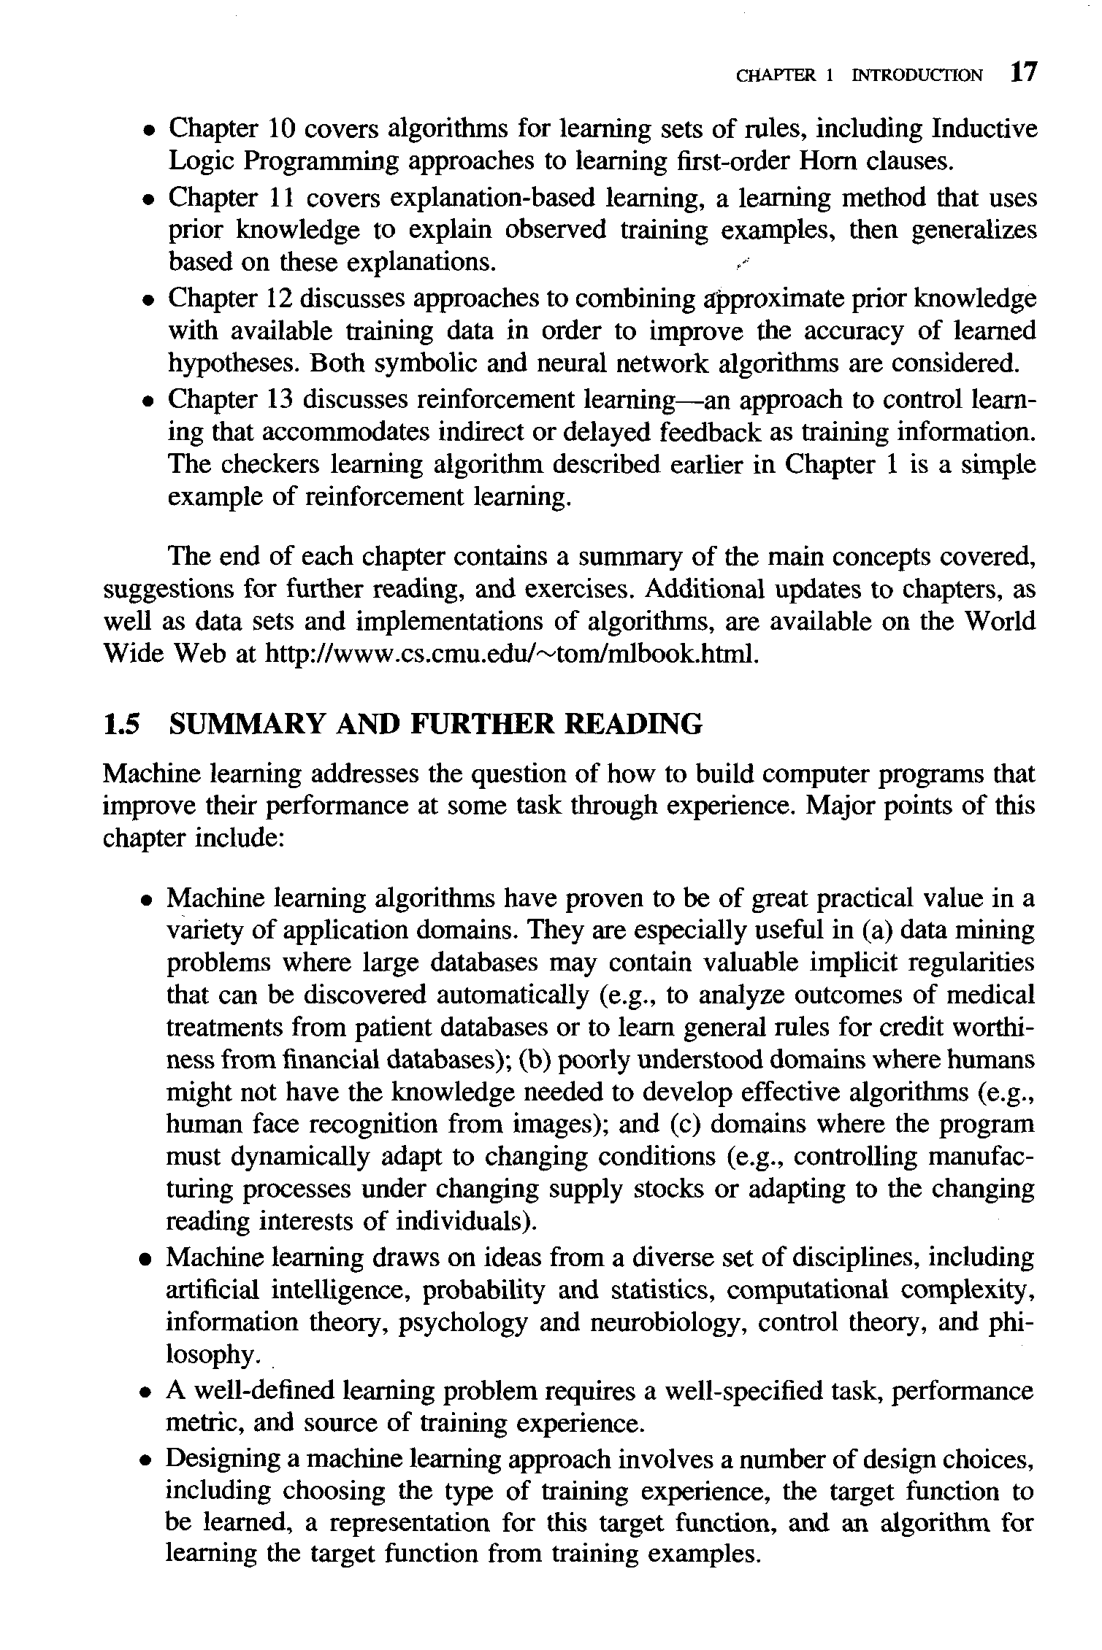
\includegraphics[width=0.9\linewidth]{figures/p29_b0.png}
\end{figure}

\section{Chương 10 trình bày các thuật toán để học các bộ quy tắc, bao gồm Quy nạp}

Phương pháp lập trình logic để học các mệnh đề Horn bậc nhất.

\section{Chương 11 đề cập đến việc học dựa trên giải thích, một phương pháp học tập sử dụng}

Kiến thức sẵn có để giải thích các ví dụ training được quan sát, sau đó khái quát hóa dựa trên những giải thích này.

\section{Chương 12 thảo luận về các phương pháp kết hợp kiến ​​thức gần đúng có sẵn}

Với dữ liệu training có sẵn nhằm nâng cao tính chính xác của các giả thuyết đã học. Cả hai thuật toán tượng trưng và neural network đều được xem xét.

\section{Chương 13 thảo luận về cách tiếp cận reinforcement learning-an để kiểm soát việc học-}

Ing chứa response gián tiếp hoặc chậm trễ dưới dạng thông tin training. Thuật toán học checkers được mô tả trước đó trong Chương 1 là một ví dụ đơn giản về reinforcement learning.

Cuối mỗi chương có phần tóm tắt các khái niệm chính được đề cập,

Gợi ý đọc thêm và bài tập. Các bản cập nhật bổ sung cho các chương, cũng như data sets và việc triển khai các thuật toán, có sẵn trên World Wide Web tại http://www.cs.cmu.edu/-tom/mlbook.html.

\subsection{SUMMARY AND FURTHER READING}

Machine learning giải quyết câu hỏi làm thế nào để xây dựng các chương trình máy tính nhằm cải thiện hiệu suất của chúng trong một số nhiệm vụ thông qua kinh nghiệm. Các điểm chính của chương này bao gồm:

Các thuật toán Machine learning đã được chứng minh là có giá trị thực tế lớn trong nhiều lĩnh vực ứng dụng. Chúng đặc biệt hữu ích trong (a) các vấn đề khai thác dữ liệu trong đó cơ sở dữ liệu lớn có thể chứa các quy tắc tiềm ẩn có giá trị có thể được phát hiện tự động (ví dụ: để phân tích outcomes về các phương pháp điều trị y tế từ cơ sở dữ liệu bệnh nhân hoặc tìm hiểu các quy tắc chung về mức độ xứng đáng tín dụng từ cơ sở dữ liệu tài chính); (b) các lĩnh vực chưa được hiểu rõ nơi con người có thể không có kiến ​​thức cần thiết để phát triển các thuật toán hiệu quả (ví dụ: nhận dạng khuôn mặt con người từ hình ảnh); và (c) các lĩnh vực mà chương trình phải thích ứng linh hoạt với các điều kiện thay đổi (ví dụ: kiểm soát quy trình sản xuất khi nguồn cung thay đổi hoặc thích ứng với sở thích đọc đang thay đổi của các cá nhân). Machine learning dựa trên ý tưởng từ nhiều lĩnh vực khác nhau, bao gồm trí tuệ nhân tạo, xác suất và thống kê, độ phức tạp tính toán, lý thuyết thông tin, tâm lý học và sinh học thần kinh, lý thuyết điều khiển và triết học.

\section{Một vấn đề học tập được xác định rõ ràng đòi hỏi một nhiệm vụ, hiệu suất được xác định rõ ràng}

Thước đo và nguồn kinh nghiệm training.

\section{Thiết kế phương pháp machine learning bao gồm một số lựa chọn thiết kế,}

Bao gồm việc chọn loại kinh nghiệm training, hàm mục tiêu cần học, cách biểu diễn hàm mục tiêu này và thuật toán học hàm mục tiêu từ các ví dụ training.

% --- page 30 ---
\section{MACHINE LEARNING}

\section{Học tập bao gồm việc tìm kiếm: tìm kiếm trong không gian của các giả thuyết khả thi}

Để tìm ra giả thuyết phù hợp nhất với các ví dụ training có sẵn và các ràng buộc hoặc kiến ​​thức có trước khác. Phần lớn cuốn sách này được sắp xếp xoay quanh các phương pháp học tập khác nhau để tìm kiếm các hypothesis spaces khác nhau (ví dụ: các không gian chứa các hàm số, neural networks, decision trees, các quy tắc ký hiệu) và xoay quanh các kết quả lý thuyết mô tả các điều kiện mà theo đó các phương pháp tìm kiếm này hội tụ về một giả thuyết tối ưu.

Có một số nguồn tốt để đọc về nghiên cứu mới nhất

Kết quả là machine learning. Các tạp chí liên quan bao gồm Machine Learning, Neural

Tính toán, Neural Networks, Tạp chí của Hiệp hội Thống kê Hoa Kỳ và Giao dịch IEEE về Phân tích Mẫu và Trí tuệ Máy. Ngoài ra còn có nhiều hội nghị thường niên đề cập đến các khía cạnh khác nhau của machine learning, bao gồm Hội nghị quốc tế về Machine Learning, Hệ thống xử lý thông tin thần kinh, Hội nghị về lý thuyết học tập tính toán, Hội nghị quốc tế về Genetic Algorithms, Hội nghị quốc tế về khám phá kiến ​​thức và khai thác dữ liệu, Hội nghị châu Âu về Machine Learning và các hội nghị khác.

\section{EXERCISES}

1.1. Hãy đưa ra ba ứng dụng máy tính mà các phương pháp tiếp cận machine learning có vẻ phù hợp.

Phù hợp và ba điều mà chúng có vẻ không phù hợp. Chọn những ứng dụng chưa được đề cập trong chương này và đưa ra lời giải thích bằng một câu cho mỗi ứng dụng.

1.2. Chọn một số nhiệm vụ học tập không được đề cập trong chương này. Mô tả nó một cách không chính thức trong một

Đoạn văn bằng tiếng Anh. Bây giờ hãy mô tả nó bằng cách nêu chính xác nhất có thể nhiệm vụ, thước đo hiệu suất và kinh nghiệm training. Cuối cùng, đề xuất một hàm mục tiêu cần học và một biểu diễn mục tiêu. Thảo luận về những sự cân bằng chính mà bạn đã cân nhắc khi xây dựng nhiệm vụ học tập này.

1.3. Chứng minh rằng quy tắc cập nhật weight LMS được mô tả trong chương này thực hiện một gradient

Giảm dần để giảm thiểu sai số bình phương. Cụ thể, xác định lỗi bình phương E như trong văn bản. Bây giờ hãy tính đạo hàm của E theo weight wi, giả sử rằng ?(b) là một hàm tuyến tính như được định nghĩa trong văn bản. Việc giảm độ dốc đạt được bằng cách cập nhật từng weight theo tỷ lệ với -e. Vì vậy, bạn phải chứng minh rằng LMS

Quy tắc training thay đổi weight theo tỷ lệ này cho mỗi mẫu training mà nó gặp.

1.4. Xem xét các chiến lược thay thế cho mô-đun Trình tạo thử nghiệm trong Hình 1.2.

Cụ thể, hãy xem xét các chiến lược trong đó Trình tạo thử nghiệm đề xuất các vị trí bảng mới bằng cách

\subsection{Tạo các vị trí hội đồng pháp lý ngẫu nhiên}

\section{Tạo thế trận bằng cách chọn trạng thái bàn cờ từ ván trước, sau đó}

Áp dụng một trong những nước đi chưa được thực hiện Chiến lược do chính bạn thiết kế

Thảo luận về sự cân bằng giữa các chiến lược này. Bạn cảm thấy điều nào sẽ hiệu quả nhất nếu số lượng ví dụ training được giữ không đổi, dựa trên thước đo hiệu suất là chiến thắng nhiều trận nhất tại giải vô địch thế giới?

1.5. Thực hiện một thuật toán tương tự như đã thảo luận cho bài toán checkers, nhưng sử dụng

Trò chơi tic-tac-toe đơn giản hơn. Biểu diễn hàm V đã học dưới dạng hàm tuyến tính

% --- page 31 ---
Sự kết hợp của bảng features theo lựa chọn của bạn. Để training chương trình của bạn, hãy phát chương trình đó nhiều lần với bản sao thứ hai của chương trình sử dụng chức năng đánh giá cố định mà bạn tạo bằng tay. Vẽ biểu đồ phần trăm số trò chơi mà hệ thống của bạn thắng so với số trò chơi training đã chơi.

\subsection{REFERENCES}

Ahn, W., \& Brewer, W. F. (1993). Nghiên cứu tâm lý về học tập dựa trên giải thích. Trong G. DeJong

(Ed.), Điều tra việc học dựa trên giải thích. Boston: Nhà xuất bản học thuật Kluwer.

Anderson, JR (1991). Vị trí của kiến ​​trúc nhận thức trong phân tích hợp lý. Trong K. VanLehn (Ed.),

Kiến trúc cho trí thông minh @p. 1-24). Hillsdale, NJ: Erlbaum.

Chi, M. T. H., \& Bassock, M. (1989). Học từ các ví dụ thông qua việc tự giải thích. Ở L. Resnick

(Ed.), Biết, học và hướng dẫn: Các tiểu luận vinh danh Robert Glaser. Hillsdale, NJ: L. Hiệp hội Erlbaum.

Cooper, G., và cộng sự. (1997). Đánh giá các phương pháp học máy để dự đoán bệnh viêm phổi

Tử vong. Trí tuệ nhân tạo trong y học, (xuất hiện).

Fayyad, U. M., Uthurusamy, R. (Biên tập) (1995). Kỷ yếu Hội nghị quốc tế lần thứ nhất về

Khám phá tri thức và khai thác dữ liệu. Công viên Menlo, CA: Báo chí AAAI.

Fayyad, U. M., Smyth, P., Weir, N., Djorgovski, S. (1995). Tự động phân tích và thăm dò

Cơ sở dữ liệu hình ảnh: Kết quả, tiến độ và thách thức. Tạp chí Hệ thống thông tin thông minh, 4, 1-19.

Laird, J., Rosenbloom, P., \& Newell, A. (1986). SOAR: Cấu trúc của một cơ chế học tập tổng quát

Nism. Machine Learning, 1(1), 1146.

Langley, P., \& Simon, H. (1995). Ứng dụng của machine learning và quy tắc quy nạp. Truyền thông-

Của ACM, 38(1 I), 55-64.

Lee, K. (1989). Nhận dạng giọng nói tự động: Sự phát triển của hệ thống Sphinx. Boston: Kluwer

Nhà xuất bản học thuật.

Pomerleau, D. A. (1989). ALVINN: Phương tiện mặt đất tự hành trong neural network. (Kỹ thuật

Báo cáo CMU-CS-89-107). Pittsburgh, PA: Đại học Carnegie Mellon.

Qin, Y., Mitchell, T., \& Simon, H. (1992). Sử dụng EBG để mô phỏng việc học của con người từ các ví dụ

Và học bằng cách làm. Kỷ yếu của Hội nghị chuyên đề nghiên cứu AI ở Florida (trang 235-239).

Rudnicky, A. I., Hauptmann, A. G., \& Lee, K. -F. (1994). Khảo sát công nghệ giọng nói hiện nay ở

Trí tuệ nhân tạo. Truyền thông của ACM, 37(3), 52-57.

Rumelhart, D., Widrow, B., \& Lehr, M. (1994). Những ý tưởng cơ bản trong neural networks. Truyền thông

Của ACM, 37(3), 87-92.

Tesauro, G. (1992). Các vấn đề thực tiễn trong học tập temporal difference. Machine Learning, 8, 257. Tesauro, G. (1995). Học Temporal difference và TD-gammon. Truyền thông của ACM,

% 38(3), 5848.
Waibel, A, Hanazawa, T., Hinton, G., Shikano, K., \& Lang, K. (1989). Nhận dạng âm vị bằng cách sử dụng

Thời gian trễ neural networks. Giao dịch IEEE về Âm học, Xử lý Lời nói và Tín hiệu, 37(3), 328-339.

% --- page 32 ---
\begin{figure}[ht]
\centering

\includegraphics[width=0.9\linewidth]{figures/p32_b0.png}
\end{figure}

\subsection{CHAPTER}

\subsection{CONCEPT LEARNING AND THE}

\subsection{GENERAL-TO-SPECIFIC 0,RDERING}

Vấn đề tạo ra các hàm tổng quát từ các ví dụ training cụ thể là vấn đề trọng tâm của việc học. Chương này xem xét concept learning: thu thập định nghĩa về một danh mục chung dựa trên một mẫu các ví dụ training tích cực và tiêu cực của danh mục đó. Concept learning có thể được xây dựng dưới dạng bài toán tìm kiếm trong một không gian xác định trước các giả thuyết tiềm năng để tìm ra giả thuyết phù hợp nhất với các ví dụ training. Trong nhiều trường hợp, việc tìm kiếm này có thể được tổ chức hiệu quả bằng cách tận dụng cấu trúc xuất hiện tự nhiên trên hypothesis space-a chung-

Theo thứ tự cụ thể của các giả thuyết. Chương này trình bày một số thuật toán học tập và xem xét các tình huống trong đó chúng hội tụ đến giả thuyết chính xác. Chúng ta cũng kiểm tra bản chất của inductive learning và lý do giải thích cho việc bất kỳ chương trình nào có thể khái quát hóa thành công ngoài dữ liệu training được quan sát.

\subsection{INTRODUCTION}

Phần lớn việc học liên quan đến việc tiếp thu các khái niệm chung từ các kỳ thi training cụ thể.

Làm ơn. Ví dụ, mọi người liên tục học các khái niệm hoặc danh mục chung như “con chim”, “ô tô”, “các tình huống mà tôi nên học thêm để vượt qua kỳ thi”, v.v. Mỗi khái niệm như vậy có thể được xem như mô tả một số tập hợp con của mục tiêu.

Các đối tượng hoặc sự kiện được xác định trên một tập hợp lớn hơn (ví dụ: tập hợp con các động vật tạo thành

% --- page 33 ---
\begin{figure}[ht]
\centering
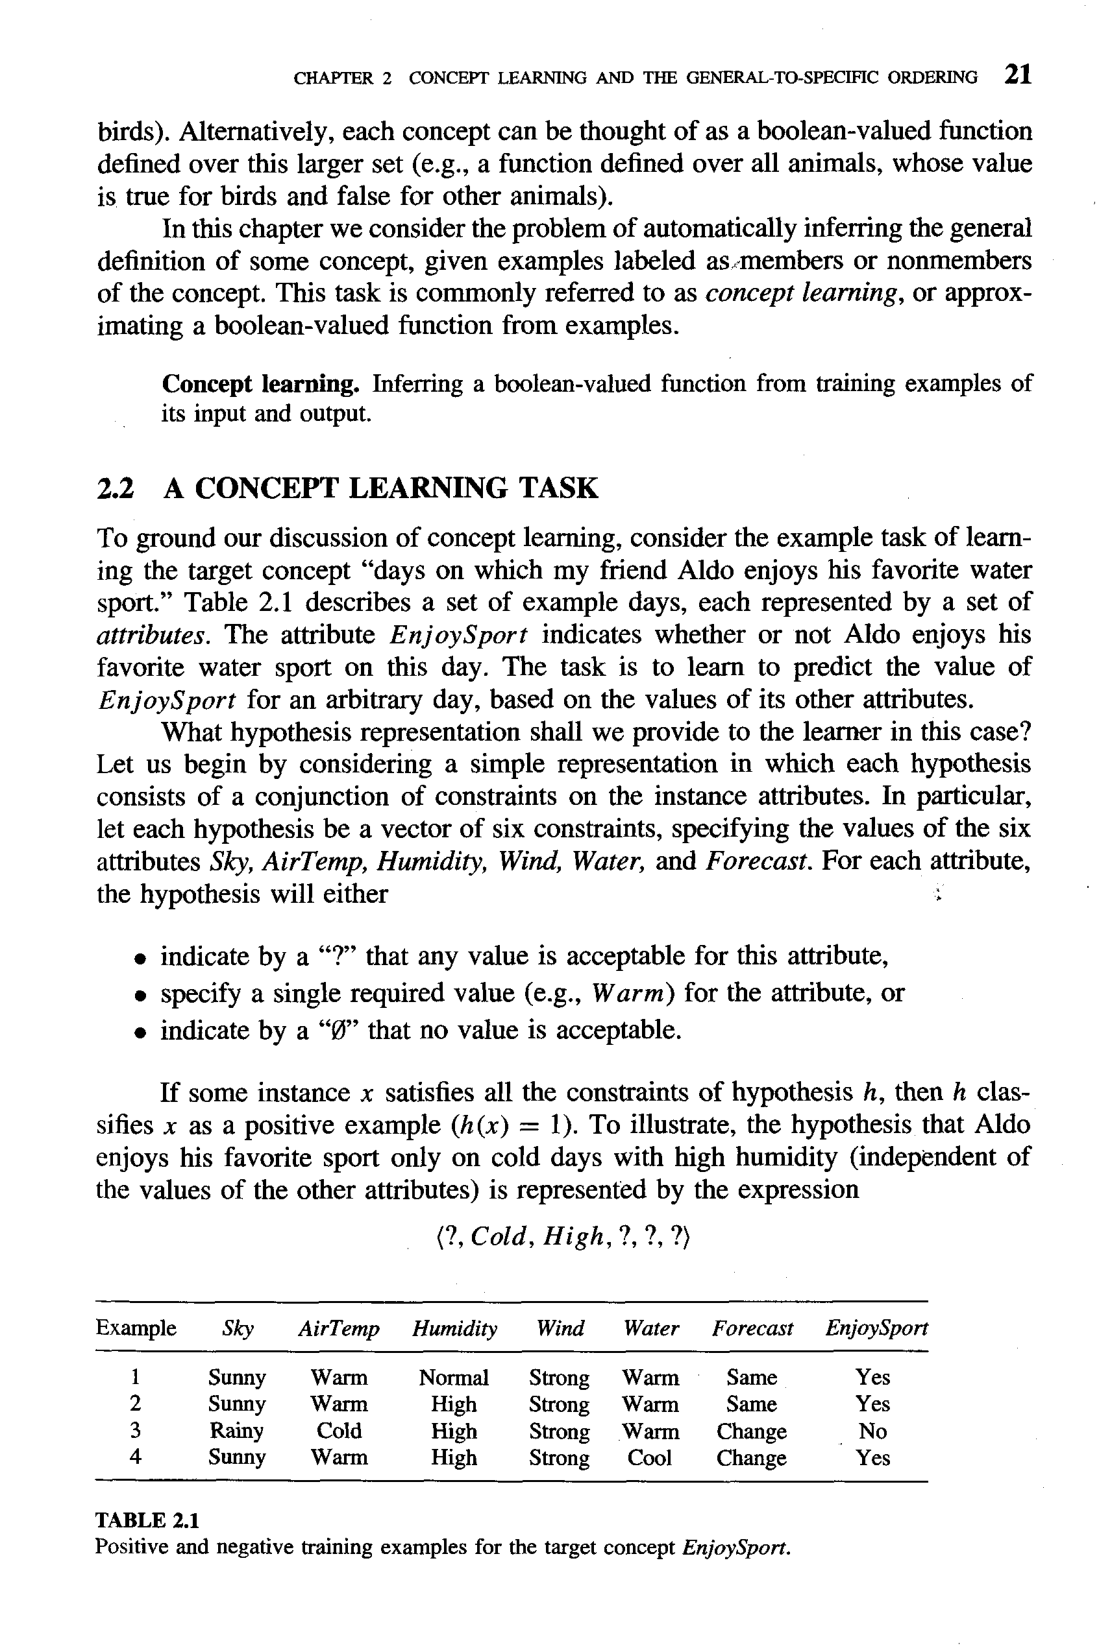
\includegraphics[width=0.9\linewidth]{figures/p33_b0.png}
\end{figure}

\subsection{CHAFER 2 CONCEm LEARNING AND THE GENERAL-TO-SPECIFIC ORDERWG 21}

Chim). Alternatively, each concept can be thought of as a boolean-valued function defined over this larger set (e.g., a function defined over all animals, whose value is true for birds and false for other animals).

Trong chương này chúng ta xem xét vấn đề tự động suy ra tổng quát

Định nghĩa của một số khái niệm, đưa ra các ví dụ được gắn nhãn là+.thành viên hoặc không phải thành viên của khái niệm đó. Tác vụ này thường được gọi là concept learning hoặc xấp xỉ hàm có giá trị boolean từ các ví dụ.

Concept learning. Suy ra hàm có giá trị boolean từ các ví dụ training của

Đầu vào và đầu ra của nó.

\subsection{A CONCEPT LEARNING TASK}

Để làm nền tảng cho cuộc thảo luận của chúng ta về concept learning, hãy xem xét nhiệm vụ mẫu là tìm hiểu khái niệm mục tiêu “những ngày mà bạn Aldo của tôi thích môn thể thao dưới nước yêu thích của mình”. Bảng 2.1 mô tả một tập hợp các ngày ví dụ, mỗi ngày được biểu thị bằng một tập hợp các

Thuộc tính. Thuộc tính EnjoySport cho biết Aldo có thích môn thể thao dưới nước yêu thích của mình vào ngày này hay không. Nhiệm vụ là học cách dự đoán giá trị của

EnjoySport cho một ngày tùy ý, dựa trên giá trị của các thuộc tính khác của nó.

Chúng ta sẽ cung cấp giả thuyết nào cho người học trong trường hợp này?

Chúng ta hãy bắt đầu bằng cách xem xét một cách biểu diễn đơn giản trong đó mỗi giả thuyết bao gồm sự kết hợp của các ràng buộc trên các thuộc tính thể hiện. Cụ thể, hãy đặt mỗi giả thuyết là một vector gồm sáu ràng buộc, chỉ định các giá trị của sáu thuộc tính Bầu trời, AirTemp, Độ ẩm, Gió, Nước và Dự báo. Đối với mỗi thuộc tính, giả thuyết sẽ

\section{biểu thị bằng dấu "?' rằng bất kỳ giá trị nào cũng được chấp nhận cho thuộc tính này,}

\section{chỉ định một giá trị bắt buộc duy nhất (ví dụ: Warm) cho thuộc tính hoặc}

\section{biểu thị bằng "0" rằng không có giá trị nào được chấp nhận.}

Nếu một số trường hợp x thỏa mãn tất cả các ràng buộc của giả thuyết h, thì h loại-

Xác định x là một ví dụ tích cực (h(x) = 1). Để minh họa, giả thuyết cho rằng Aldo chỉ thích môn thể thao yêu thích của mình vào những ngày lạnh giá với độ ẩm cao (không phụ thuộc vào giá trị của các thuộc tính khác) được biểu thị bằng biểu thức

(?, Lạnh, Cao, ?, ?, ?)

Ví dụ Bầu trời AirTemp Độ ẩm Gió Nước Dự báo EnjoySport

\section{Nắng Ấm Bình thường Mạnh Ấm Tương tự Có}

\section{Nắng Ấm Cao Mạnh Ấm Tương tự Có}

\section{Mưa Lạnh Cao Mạnh Ấm Thay đổi Không}

\section{Nắng Ấm Cao Mạnh Mát Thay đổi Có}

\noindent\textit{TABLE 2.1 Các ví dụ training tích cực và tiêu cực cho khái niệm mục tiêu EnjoySport.}

% --- page 34 ---
\begin{figure}[ht]
\centering

\includegraphics[width=0.9\linewidth]{figures/p34_b0.png}
\end{figure}

\section{MACHINE LEARNING}

Giả thuyết chung nhất – rằng mỗi ngày đều là một tấm gương tích cực – đại diện cho

\subsection{Gửi bởi}

(?, ?, ?, ?, ?, ?)

Và giả thuyết cụ thể nhất có thể có – rằng không có ngày nào là ví dụ tích cực – là

\subsection{Đại diện bởi}

% (0,0,0,0,0,0)
Tóm lại, nhiệm vụ EnjoySport concept learning yêu cầu học các

Tập hợp các ngày mà EnjoySport = có, mô tả tập hợp này bằng sự kết hợp của các ràng buộc đối với các thuộc tính mẫu. Nói chung, bất kỳ nhiệm vụ concept learning nào cũng có thể được mô tả bằng tập hợp các trường hợp mà hàm mục tiêu được xác định, hàm mục tiêu, tập hợp các giả thuyết ứng cử viên được người học xem xét và tập hợp các ví dụ training có sẵn. Định nghĩa của nhiệm vụ EnjoySport concept learning ở dạng chung này được đưa ra trong Bảng 2.2.

\subsubsection{Ký hiệu}

Trong suốt cuốn sách này, chúng ta sử dụng thuật ngữ sau khi thảo luận về các bài toán concept learning. Tập hợp các mục mà khái niệm được xác định được gọi là tập hợp các trường hợp, được biểu thị bằng X. Trong ví dụ hiện tại, X là tập hợp tất cả các ngày có thể, mỗi ngày được biểu thị bằng các thuộc tính Sky, AirTemp,

Độ ẩm, Gió, Nước và Dự báo. Khái niệm hoặc chức năng cần học là

Được gọi là khái niệm mục tiêu, mà chúng ta biểu thị bằng c. Nói chung, c có thể là bất kỳ hàm có giá trị boolean nào được xác định trên các thể hiện X; tức là c : X + \{O, 1). Trong ví dụ hiện tại, khái niệm đích tương ứng với giá trị của thuộc tính EnjoySport (nghĩa là c(x) = 1 nếu EnjoySport = Có và c(x) = 0 nếu EnjoySport = Không).

% -
\section{Đã cho:}

\section{Trường hợp X: Ngày có thể, mỗi trường hợp được mô tả bằng thuộc tính}

\section{Bầu trời (với các giá trị có thể có Nắng, Mây và Mưa),}

\section{AirTemp (có giá trị Ấm và Lạnh),}

\section{Độ ẩm (có giá trị Bình thường và Cao),}

\section{Gió (có giá trị Mạnh và Yếu),}

\section{Nước (có giá trị Ấm và Mát) và}

\section{Dự báo (với các giá trị Tương tự và Thay đổi).}

\section{Giả thuyết H: Mỗi giả thuyết được mô tả bằng sự kết hợp của các ràng buộc trên}

Tôn vinh Bầu trời, AirTemp, Độ ẩm, Gió, Nước và Dự báo. Các ràng buộc có thể là "?" (bất kỳ giá trị nào cũng được chấp nhận), " 0 (không có giá trị nào được chấp nhận) hoặc một giá trị cụ thể.

\section{Khái niệm mục tiêu c: EnjoySport : X + (0,l)}

\section{Ví dụ training D: Ví dụ dương và âm của hàm mục tiêu (xem Bảng 2.1).}

\section{Xác định:}

\[0 A hypothesis h in H such that h(x) = c(x) for all x in X.\]

\noindent\textit{TABLE 2.2 Nhiệm vụ EnjoySport concept learning.}

% --- page 35 ---
\begin{figure}[ht]
\centering
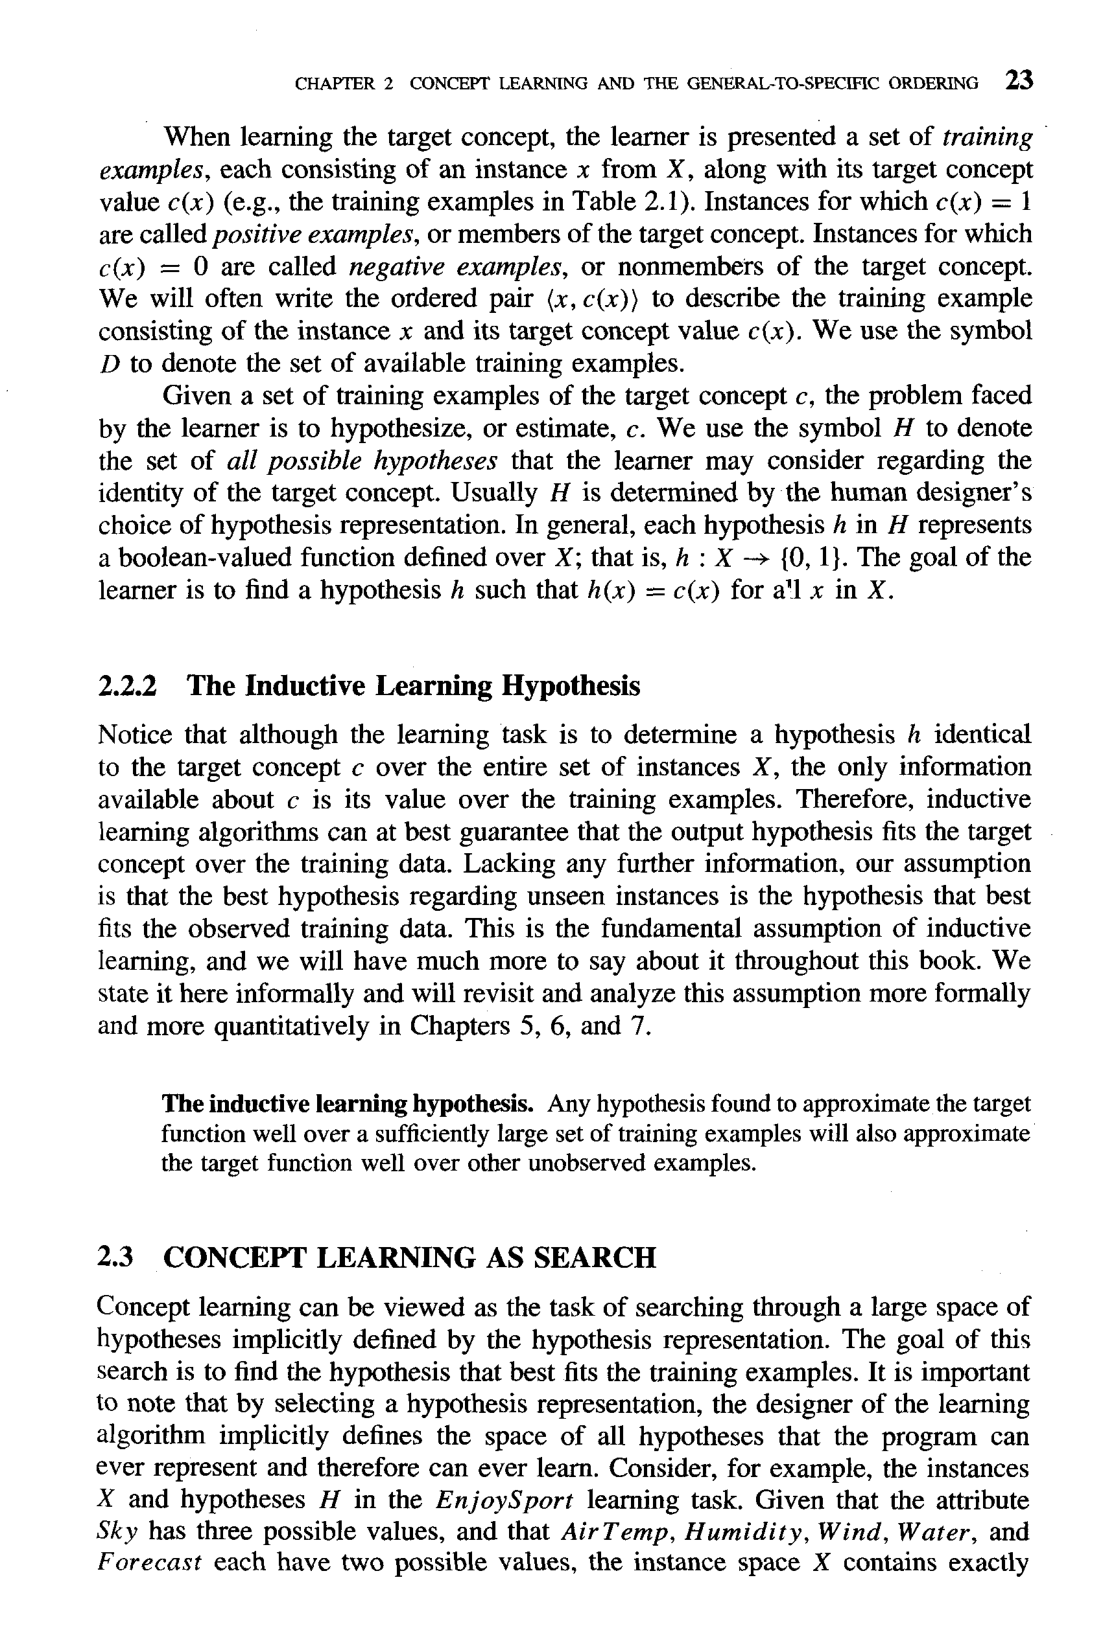
\includegraphics[width=0.9\linewidth]{figures/p35_b0.png}
\end{figure}

Khi học khái niệm mục tiêu, người học được cung cấp một tập các bài tập training

Các ví dụ, mỗi ví dụ bao gồm một thể hiện x từ X, cùng với giá trị khái niệm đích c(x) của nó (ví dụ: các ví dụ training trong Bảng 2.1). Các trường hợp c(x) = 1 được gọi là các ví dụ tích cực hoặc các thành viên của khái niệm đích. Các trường hợp mà C ( X ) = 0 được gọi là ví dụ phủ định hoặc không phải là thành viên của khái niệm đích. Chúng ta thường viết cặp có thứ tự (x, c(x)) để mô tả ví dụ training bao gồm individual x và giá trị khái niệm đích của nó là c(x). Chúng ta sử dụng ký hiệu

D để biểu thị tập hợp các ví dụ training có sẵn.

Đưa ra một tập hợp các ví dụ training về khái niệm mục tiêu c, vấn đề phải đối mặt

Do người học thực hiện là đưa ra giả thuyết, hoặc estimate, c. Chúng ta sử dụng ký hiệu H để biểu thị tập hợp tất cả các giả thuyết có thể có mà người học có thể xem xét liên quan đến việc nhận dạng khái niệm mục tiêu. Thông thường H được xác định bởi sự lựa chọn trình bày giả thuyết của người thiết kế con người. Nói chung, mỗi giả thuyết h trong H đại diện cho một hàm có giá trị boolean được xác định trên X; tức là h : X --+ \{O, 1). Mục tiêu của người học là tìm ra giả thuyết h sao cho h(x) = c(x) với a" x trong X.

\subsubsection{Giả thuyết Inductive Learning}

Lưu ý rằng mặc dù nhiệm vụ học tập là xác định giả thuyết h giống với khái niệm đích c trên toàn bộ tập hợp các trường hợp X, thông tin duy nhất có được về c là giá trị của nó trên các ví dụ training. Do đó, thuật toán inductive learning có thể đảm bảo tốt nhất rằng giả thuyết đầu ra phù hợp với khái niệm mục tiêu trên dữ liệu training. Thiếu bất kỳ thông tin nào khác, giả định của chúng ta là giả thuyết tốt nhất về các trường hợp chưa được nhìn thấy là giả thuyết phù hợp nhất với dữ liệu training được quan sát. Đây là giả định cơ bản của inductive learning và chúng ta sẽ còn nhiều điều để nói về nó trong suốt cuốn sách này. Chúng ta trình bày nó ở đây một cách không chính thức và sẽ xem xét lại cũng như phân tích giả định này một cách chính thức hơn và định lượng hơn trong các Chương 5, 6 và 7.

Giả thuyết inductive learning. Bất kỳ giả thuyết nào được tìm thấy gần đúng với hàm mục tiêu trên một tập hợp các ví dụ training đủ lớn cũng sẽ gần đúng với hàm mục tiêu so với các ví dụ không được quan sát khác.

\subsection{CONCEPT LEARNING AS SEARCH}

Concept learning có thể được coi là nhiệm vụ tìm kiếm trong một không gian rộng lớn các giả thuyết được xác định ngầm bởi cách biểu diễn giả thuyết. Mục tiêu của việc tìm kiếm này là tìm ra giả thuyết phù hợp nhất với các ví dụ training. Điều quan trọng cần lưu ý là bằng cách chọn cách biểu diễn giả thuyết, người thiết kế thuật toán học đã ngầm xác định không gian của tất cả các giả thuyết mà chương trình có thể biểu diễn và do đó có thể học. Ví dụ, hãy xem xét các trường hợp X và giả thuyết H trong nhiệm vụ học tập EnjoySport. Cho rằng thuộc tính Bầu trời có ba giá trị có thể có và AirTemp, Độ ẩm, Gió, Nước và

Dự báo mỗi giá trị có hai giá trị có thể, không gian thể hiện X chứa chính xác

% --- page 36 ---
\begin{figure}[ht]
\centering
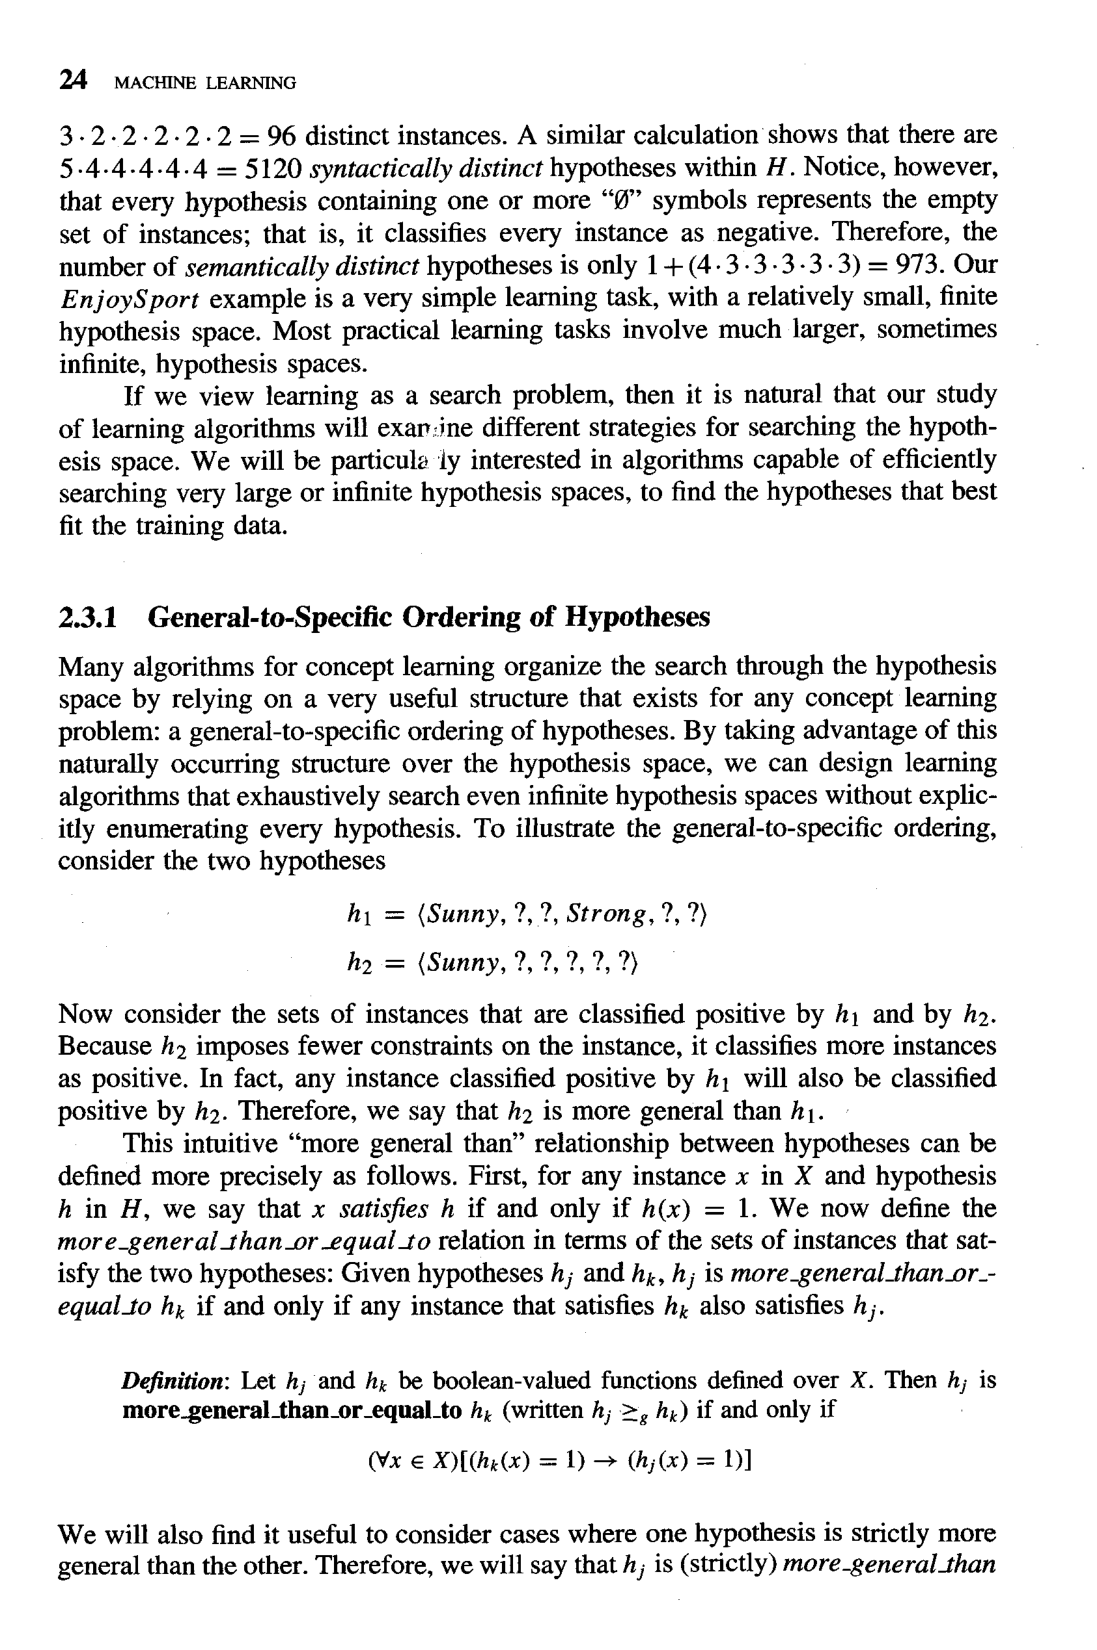
\includegraphics[width=0.9\linewidth]{figures/p36_b0.png}
\end{figure}

\section{.2 2 . 2 2 . 2 = 96 trường hợp riêng biệt. Một tính toán tương tự cho thấy có 5,4-4 - 4 -4,4 = 5 120 giả thuyết khác biệt về mặt cú pháp trong H. Tuy nhiên, lưu ý rằng mọi giả thuyết chứa một hoặc nhiều ký hiệu "IZI" đại diện cho tập hợp các trường hợp trống; nghĩa là nó classification mọi trường hợp là tiêu cực. Vì vậy,}

\[number of semantically distinct hypotheses is only 1 + (4.3.3.3.3.3) = 973. Our\]

Ví dụ EnjoySport là một nhiệm vụ học tập rất đơn giản, với kích thước tương đối nhỏ và hữu hạn.

Hypothesis space. Hầu hết các nhiệm vụ học tập thực tế đều liên quan đến hypothesis spaces lớn hơn nhiều, đôi khi là vô hạn.

Nếu chúng ta xem việc học như một vấn đề tìm kiếm thì điều tự nhiên là nghiên cứu của chúng ta

Thuật toán học sẽ giải thích các chiến lược khác nhau để tìm kiếm hypothesis space. Chúng ta sẽ đặc biệt quan tâm đến các thuật toán có khả năng tìm kiếm hypothesis spaces rất lớn hoặc vô hạn một cách hiệu quả, để tìm ra các giả thuyết phù hợp nhất với dữ liệu training.

\subsubsection{Thứ tự các giả thuyết từ tổng quát đến cụ thể}

Nhiều thuật toán cho concept learning tổ chức tìm kiếm thông qua giả thuyết

Không gian bằng cách dựa vào cấu trúc rất hữu ích tồn tại cho mọi concept learning

Vấn đề: sự sắp xếp các giả thuyết từ tổng thể đến cụ thể. Bằng cách tận dụng cấu trúc xuất hiện tự nhiên này trên hypothesis space, chúng ta có thể thiết kế các thuật toán học tìm kiếm một cách toàn diện ngay cả hypothesis spaces vô hạn mà không cần giải thích.

Nó liệt kê mọi giả thuyết. Để minh họa thứ tự từ tổng quát đến cụ thể, hãy xem xét hai giả thuyết

Chào = (Sunny, ?, ?, Mạnh mẽ, ?, ?)

H2 = (Nắng, ?, ?, ?, ?, ?)

Bây giờ hãy xem xét tập hợp các trường hợp được phân loại dương bởi hl và h2. Vì h2 áp đặt ít ràng buộc hơn cho phiên bản nên nó classification nhiều phiên bản hơn là tích cực. Trên thực tế, bất kỳ trường hợp nào được phân loại tích cực bởi hl cũng sẽ được h2 classification tích cực. Vì vậy, chúng ta nói rằng h2 tổng quát hơn hl.

Mối quan hệ “tổng quát hơn” trực quan này giữa các giả thuyết có thể được

Được xác định chính xác hơn như sau. Đầu tiên, với mọi trường hợp x trong X và giả thuyết h trong H, chúng ta nói rằng x thỏa mãn h khi và chỉ khi h(x) = 1. Bây giờ chúng ta định nghĩa mối quan hệ tổng quát hơn\textasciitilde{}han\_or.-bằng\textasciitilde{}o theo các tập hợp trường hợp thỏa mãn

Thỏa mãn hai giả thuyết: Cho giả thuyết hj và hk, hj tổng quát hơn bằng hk khi và chỉ khi bất kỳ trường hợp nào thỏa mãn hk cũng thỏa mãn hi.

Định nghĩa: Cho hj và hk là các hàm có giá trị boolean được xác định trên X. Khi đó hj là

Tổng quát hơn hoặc bằng hk (viết hj 2, hk) khi và chỉ khi

Chúng ta cũng sẽ thấy hữu ích khi xem xét các trường hợp trong đó một giả thuyết hoàn toàn tổng quát hơn giả thuyết kia. Vì vậy, chúng ta sẽ nói rằng hj (đúng) tổng quát hơndhan

% --- page 37 ---
\begin{figure}[ht]
\centering
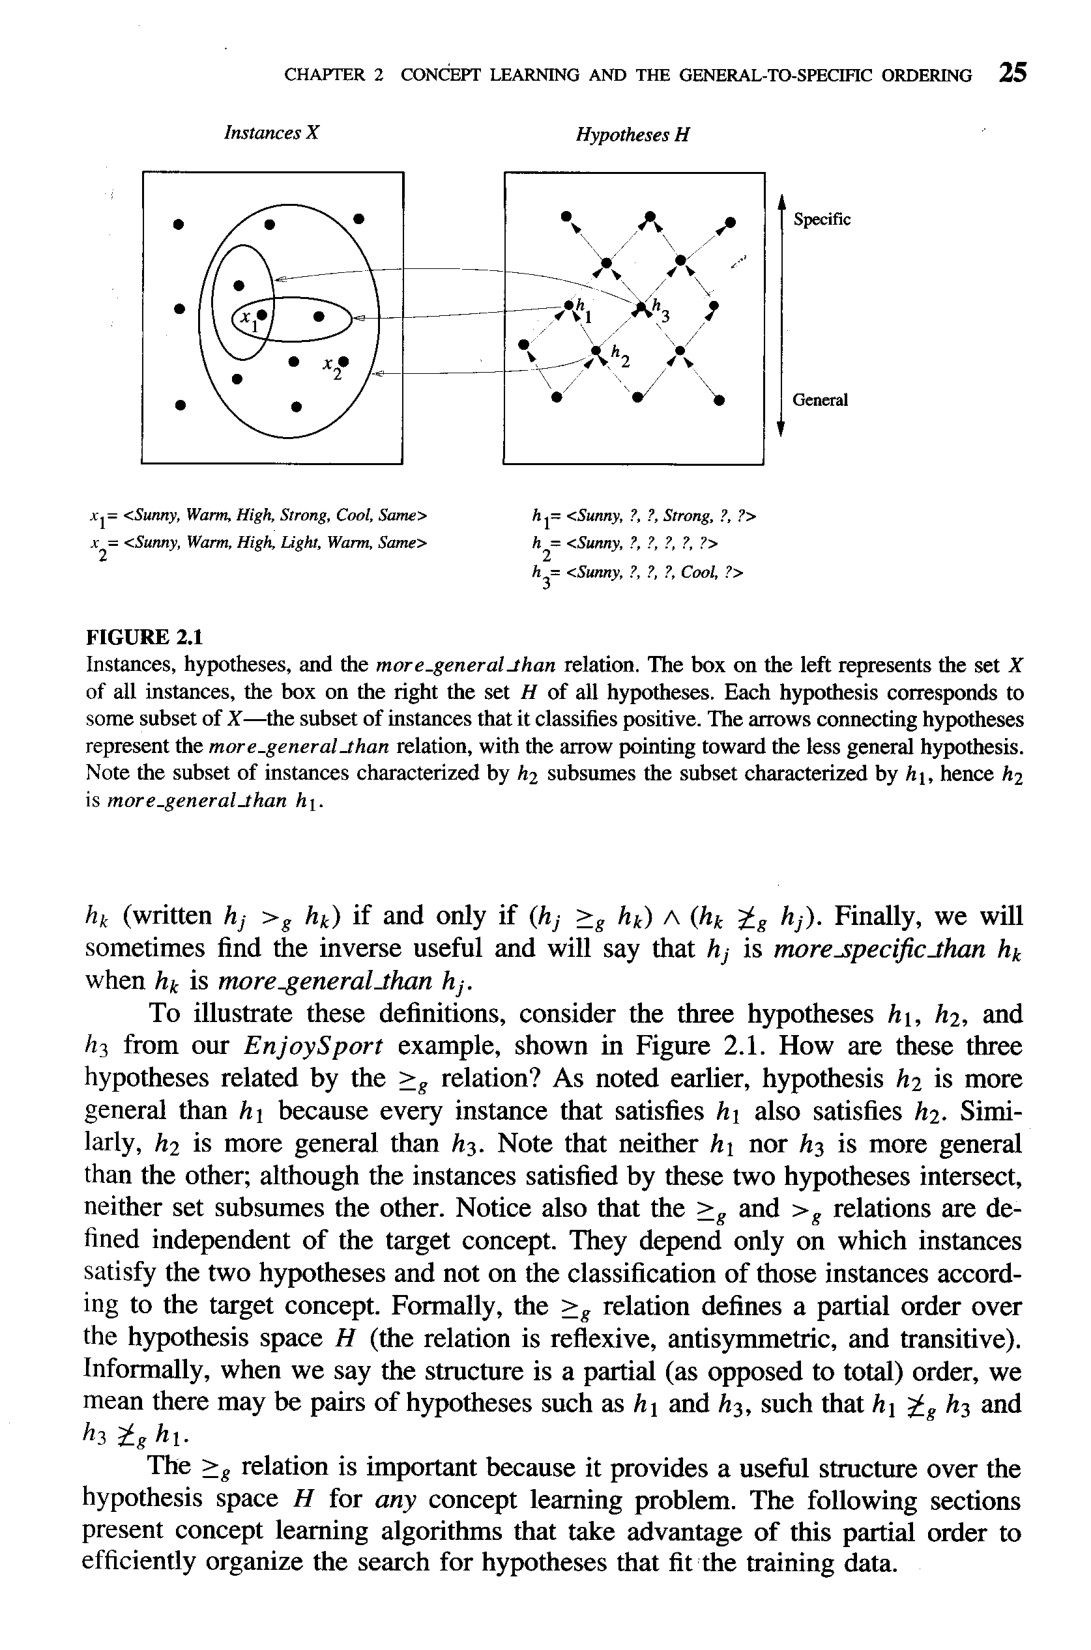
\includegraphics[width=0.9\linewidth]{figures/p37_b0.png}
\end{figure}

\subsection{CHAPTER 2 CONCEPT LEARNING AND THE GENERAL-TO-SPECIFIC ORDERING 25}

Tầm ảnh hưởng X Giả thuyết H

Tôi tôi

MỘT

Cụ thể

Tổng quan

T

Tôi

XI= <Nắng, W a n , Cao, Mạnh, Mát, Tương tự> hl= <Nắng, ?, ?, Mạnh, ?, ?>

X = <Nắng, Ấm áp, Cao, Nhẹ, Ấm áp, Tương tự> 2 h = <Nắng, ?, ?, ?, ?, ?> 2

H 3 = <Nắng, ?, ?, 7, Mát mẻ, ?>

\noindent\textit{FIGURE 2.1 Các trường hợp, giả thuyết và mối quan hệ đa dạng hơn. Hộp bên trái đại diện cho tập X của tất cả các trường hợp, hộp bên phải là tập H của tất cả các giả thuyết. Mỗi giả thuyết tương ứng với một tập hợp con nào đó của X - tập hợp con của các trường hợp mà nó được phân loại là tích cực. Các mũi tên kết nối các giả thuyết}

Biểu diễn mối quan hệ nhiều hơn, nhiều hơn, với mũi tên hướng về giả thuyết ít tổng quát hơn. Lưu ý tập hợp con của các trường hợp được feature bởi h2 gộp lại tập hợp con được feature bởi h l , do đó h2 là m o r e - g e n e r a l - t ha n h l .

Hk (viết hj >, hk) khi và chỉ khi (hj p, hk) A (hk 2, hi). Cuối cùng, đôi khi chúng ta sẽ thấy nghịch đảo hữu ích và sẽ nói rằng hj đặc biệt hơn hk khi hk là more\_general-than hj.

Để minh họa các định nghĩa này, hãy xem xét ba giả thuyết hl, h2 và

H3 từ ví dụ về Enjoysport của chúng ta, được hiển thị trong Hình 2.1. Ba giả thuyết này có liên quan như thế nào bởi mối quan hệ p? Như đã lưu ý trước đó, giả thuyết h2 tổng quát hơn hl vì mọi trường hợp thỏa mãn hl cũng thỏa mãn h2. Tương tự, h2 tổng quát hơn h3. Lưu ý rằng cả hl và h3 đều không chung chung hơn cái kia; mặc dù các trường hợp được thỏa mãn bởi hai giả thuyết này giao nhau, nhưng không tập nào gộp tập kia. Cũng lưu ý rằng các mối quan hệ p và > được xác định độc lập với khái niệm đích. Chúng chỉ phụ thuộc vào trường hợp nào thỏa mãn hai giả thuyết chứ không phụ thuộc vào classification của các trường hợp đó theo khái niệm mục tiêu. Về mặt hình thức, quan hệ p xác định một phần trật tự trên hypothesis space H (quan hệ phản xạ, phản đối xứng và bắc cầu). Một cách không chính thức, khi chúng ta nói cấu trúc là một trật tự một phần (ngược lại với tổng), chúng ta muốn nói rằng có thể có các cặp giả thuyết như hl và h3, chẳng hạn như hl 2, h3 và h3 2, hl.

Mối quan hệ pg rất quan trọng vì nó cung cấp một cấu trúc hữu ích trên

Hypothesis space H cho mọi vấn đề về concept learning. Các phần sau đây trình bày các thuật toán concept learning tận dụng thứ tự một phần này để tổ chức hiệu quả việc tìm kiếm các giả thuyết phù hợp với dữ liệu training.

% --- page 38 ---
\begin{figure}[ht]
\centering
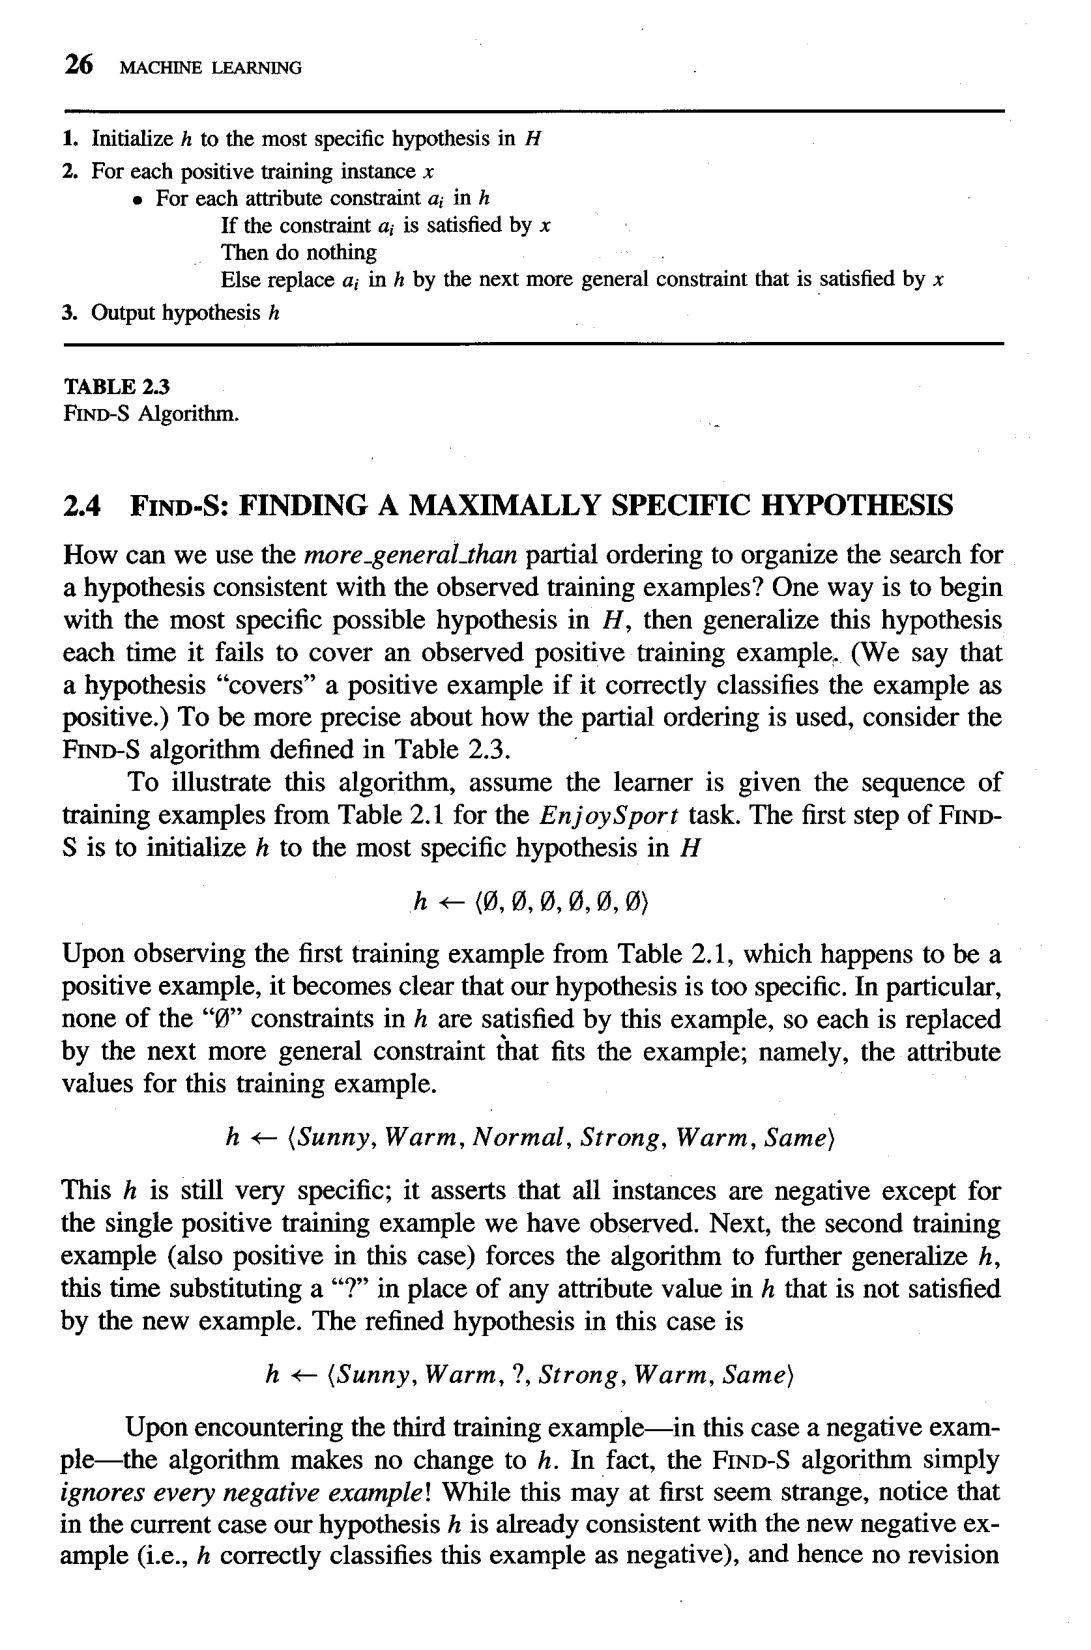
\includegraphics[width=0.9\linewidth]{figures/p38_b0.png}
\end{figure}

1. Khởi tạo h thành giả thuyết cụ thể nhất trong H 2. Với mỗi trường hợp training tích cực x

\section{Với mỗi ràng buộc thuộc tính a, trong h}

Nếu ràng buộc a, được x thỏa mãn thì không làm gì cả Thay thế a, trong h bằng ràng buộc tổng quát hơn tiếp theo được x thỏa mãn

3. Giả thuyết đầu ra h

\noindent\textit{Thuật toán TABLE 2.3 FIND-S.}

\subsection{FIND-S: FINDING A MAXIMALLY SPECIFIC HYPOTHESIS}

Làm cách nào chúng ta có thể sử dụng thứ tự tổng quát hơn từng phần để tổ chức tìm kiếm giả thuyết phù hợp với các ví dụ training được quan sát? Một cách là bắt đầu với giả thuyết cụ thể nhất có thể có trong H, sau đó khái quát hóa giả thuyết này mỗi khi nó không bao gồm được một ví dụ training tích cực được quan sát. (Chúng ta nói rằng một giả thuyết "bao trùm" một ví dụ tích cực nếu nó classification chính xác ví dụ đó là

Tích cực.) Để chính xác hơn về cách sử dụng thứ tự từng phần, hãy xem xét thuật toán FIND-S được xác định trong Bảng 2.3.

Để minh họa thuật toán này, giả sử người học được cung cấp chuỗi các

Ví dụ training từ Bảng 2.1 cho nhiệm vụ EnjoySport. Bước đầu tiên của FINDS là khởi tạo h thành giả thuyết cụ thể nhất trong H

Khi quan sát ví dụ training đầu tiên từ Bảng 2.1, đây là một ví dụ tích cực, có thể thấy rõ rằng giả thuyết của chúng ta quá cụ thể. Đặc biệt, không có ràng buộc "0" nào trong h được ví dụ này thỏa mãn, vì vậy mỗi ràng buộc được thay thế bằng ràng buộc tổng quát hơn tiếp theo \{hat phù hợp với ví dụ; cụ thể là các giá trị thuộc tính cho ví dụ training này.

\subsection{H -+ (Nắng, Ấm áp, Bình thường, Mạnh mẽ, Ấm áp, Tương tự)}

H này vẫn rất cụ thể; nó khẳng định rằng tất cả các trường hợp đều tiêu cực ngoại trừ ví dụ training tích cực duy nhất mà chúng ta đã quan sát. Tiếp theo, ví dụ training thứ hai (cũng tích cực trong trường hợp này) buộc thuật toán phải tổng quát hóa h hơn, lần này thay thế một "?' thay cho bất kỳ giá trị thuộc tính nào trong h mà mẫu mới không thỏa mãn. Giả thuyết tinh tế trong trường hợp này là

H -+ (Nắng, Ấm áp, ?, Mạnh mẽ, Ấm áp, Tương tự)

Khi gặp ví dụ training thứ ba - trong trường hợp này là một bài kiểm tra tiêu cực-

Ple-thuật toán không làm thay đổi h. Trên thực tế, thuật toán FIND-S chỉ đơn giản là

Bỏ qua mọi ví dụ tiêu cực! Mặc dù điều này lúc đầu có vẻ lạ lùng nhưng hãy chú ý rằng

Trong trường hợp hiện tại, giả thuyết h của chúng ta đã nhất quán với ví dụ phủ định mới (tức là h classification chính xác ví dụ này là phủ định) và do đó không cần sửa đổi

% --- page 39 ---
\begin{figure}[ht]
\centering
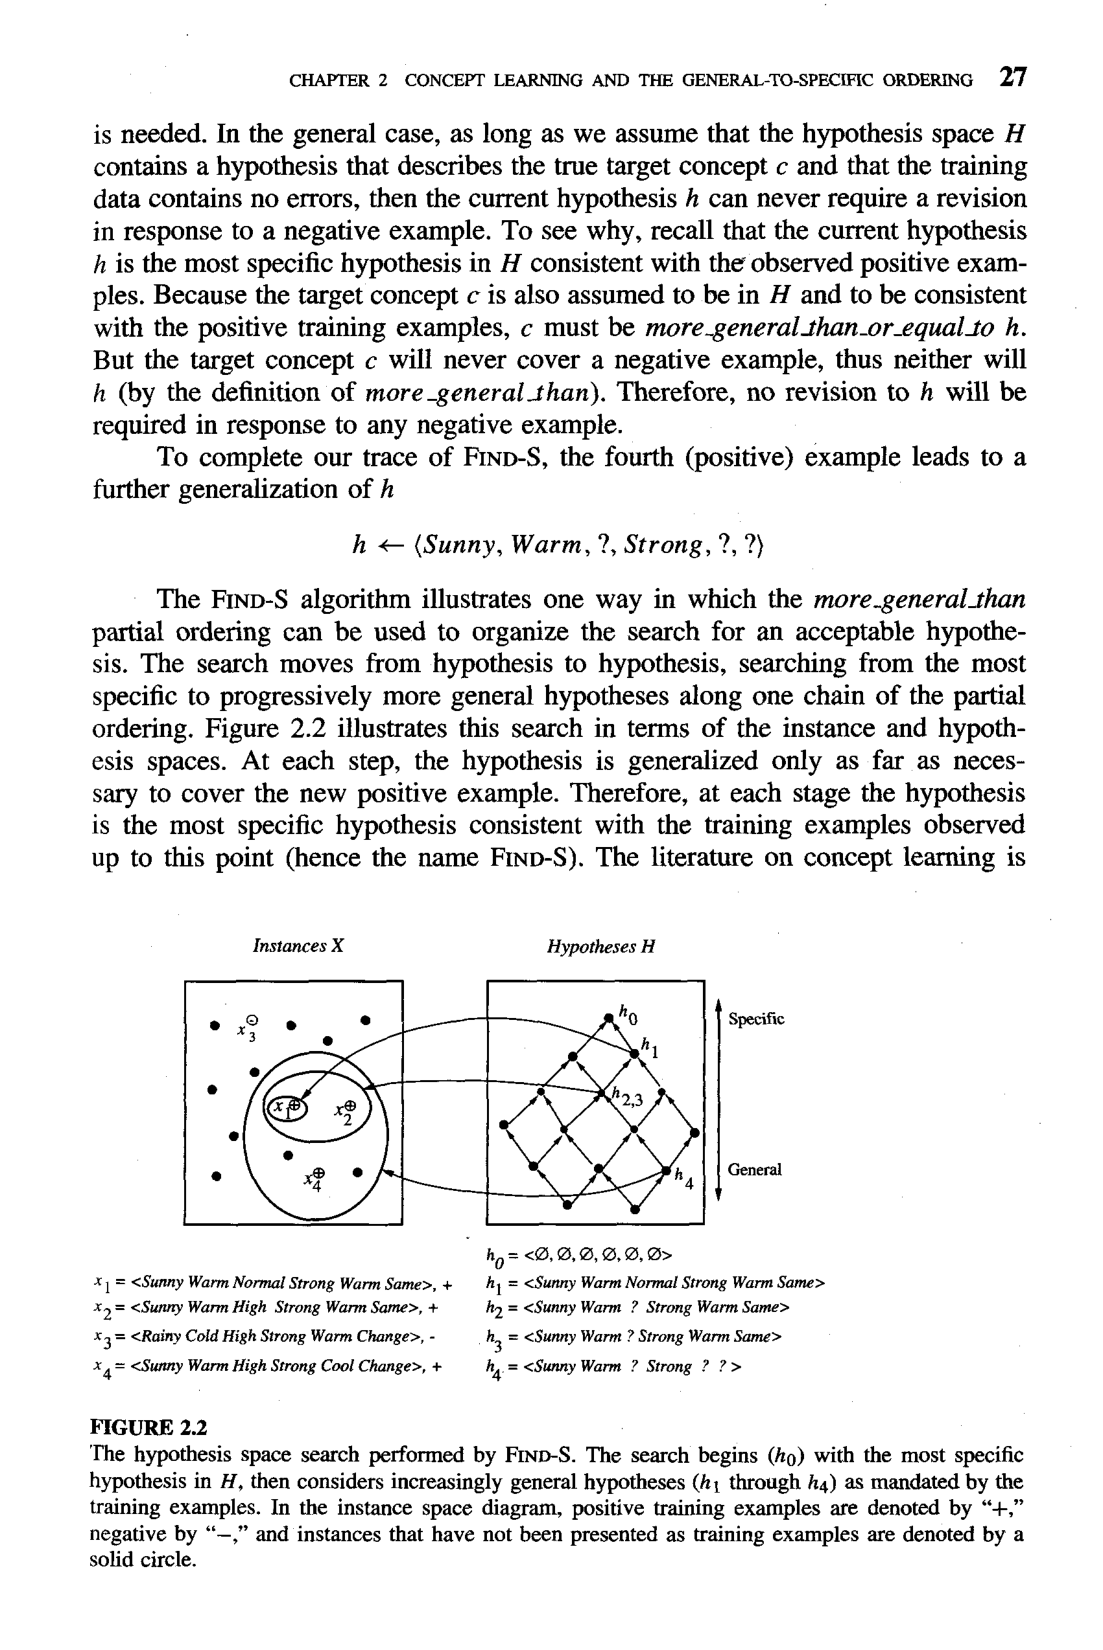
\includegraphics[width=0.9\linewidth]{figures/p39_b0.png}
\end{figure}

Là cần thiết. Trong trường hợp tổng quát, miễn là chúng ta giả sử rằng hypothesis space H chứa giả thuyết mô tả khái niệm mục tiêu thực sự c và dữ liệu training không có lỗi thì giả thuyết hiện tại h không bao giờ có thể yêu cầu sửa đổi response thành một ví dụ phủ định. Để biết lý do tại sao, hãy nhớ lại rằng giả thuyết hiện tại h là giả thuyết cụ thể nhất trong H phù hợp với các ví dụ tích cực được quan sát. Vì khái niệm đích c cũng được giả định là thuộc H và để nhất quán với các ví dụ training tích cực nên c phải lớn hơn.general\_than-or-equaldo h.

Nhưng khái niệm mục tiêu c sẽ không bao giờ bao hàm một ví dụ tiêu cực, do đó h cũng vậy (theo định nghĩa tổng quát hơn\textasciitilde{}han). Do đó, không cần sửa đổi h trong response đối với bất kỳ ví dụ phủ định nào.

Để hoàn thành việc theo dõi FIND-S của chúng ta, ví dụ thứ tư (tích cực) dẫn đến một

\subsection{Khái quát hóa hơn nữa của h}

H t (Nắng, Ấm áp, ?, Mạnh mẽ, ?, ?)

Thuật toán FIND-S minh họa một cách trong đó thuật toán tổng quát hơn

Việc sắp xếp từng phần có thể được sử dụng để tổ chức việc tìm kiếm một giả thuyết có thể chấp nhận được.

Chị ơi. Việc tìm kiếm chuyển từ giả thuyết này sang giả thuyết khác, tìm kiếm từ giả thuyết cụ thể nhất đến giả thuyết tổng quát hơn theo một chuỗi trật tự từng phần. Hình 2.2 minh họa tìm kiếm này theo thể hiện và hypothesis spaces. Ở mỗi bước, giả thuyết chỉ được khái quát hóa ở mức độ cần thiết.

Sary để đề cập đến ví dụ tích cực mới. Vì vậy, ở mỗi giai đoạn, giả thuyết

Là giả thuyết cụ thể nhất phù hợp với các ví dụ training được quan sát cho đến thời điểm này (do đó có tên FIND-S). Tài liệu về concept learning là

Trường hợp X Giả thuyết H

Cụ thể

Tổng quan

* 1 = <Nắng Ấm Bình Thường Mạnh Ấm Tương Tự>, + h, = <Nắng Ấm Bình Thường Mạnh Ấm Tương Tự>

$X_{2}$ = <Nắng Ấm Cao Mạnh Ấm Tương tự>, + h2 = <Nắng Ấm ? Mạnh mẽ ấm áp tương tự>

$X_{3}$ = <Mưa Lạnh Cao Thay Đổi Ấm Mạnh>, h = <Nắng Ấm ? Mạnh Ấm Tương tự> 3

X - <Nắng Ấm Cao Mạnh Thay Đổi Mát>, + h - <Nắng Ấm ? Mạnh ? ? > 44 -

\noindent\textit{FIGURE 2.2 'Tìm kiếm hypothesis space được thực hiện bởi FINDS. Việc tìm kiếm bắt đầu (ho) với giả thuyết cụ thể nhất trong H, sau đó xem xét các giả thuyết tổng quát hơn (hl đến h4) theo yêu cầu của các ví dụ training. Trong sơ đồ version space, các mẫu training tích cực được biểu thị bằng "+", âm bởi "-" và các trường hợp chưa được trình bày dưới dạng mẫu training được biểu thị bằng một vòng tròn liền nét.}

% --- page 40 ---
\begin{figure}[ht]
\centering

\includegraphics[width=0.9\linewidth]{figures/p40_b0.png}
\end{figure}

Được phổ biến bởi nhiều thuật toán khác nhau sử dụng cùng thứ tự tổng quát hơn một phần này để tổ chức tìm kiếm theo cách này hay cách khác. Một số thuật toán như vậy sẽ được thảo luận trong chương này và một số thuật toán khác được trình bày trong

Chương 10.

Thuộc tính chính của thuật toán FIND-S là dành cho hypothesis spaces de-

Được viết bằng các liên kết của các ràng buộc thuộc tính (chẳng hạn như H cho nhiệm vụ EnjoySport), FIND-S được đảm bảo đưa ra giả thuyết cụ thể nhất trong H phù hợp với các ví dụ training tích cực. Giả thuyết cuối cùng của nó cũng sẽ nhất quán với các ví dụ tiêu cực với điều kiện mục tiêu chính xác.

Cept được chứa trong H và miễn là các ví dụ training là chính xác. Tuy nhiên, vẫn còn một số câu hỏi chưa được giải đáp bằng thuật toán học tập này, chẳng hạn như:

Người học đã hội tụ được đúng khái niệm mục tiêu chưa? Mặc dù FIND-S sẽ tìm ra giả thuyết phù hợp với dữ liệu training, nhưng nó không có cách nào để xác định liệu nó có tìm thấy giả thuyết duy nhất trong H phù hợp với dữ liệu hay không (tức là khái niệm mục tiêu chính xác) hoặc liệu có nhiều giả thuyết nhất quán khác hay không. Chúng ta muốn một thuật toán học có thể xác định liệu nó có hội tụ hay không và nếu không thì ít nhất cũng mô tả được tính chất không chắc chắn của nó liên quan đến danh tính thực sự của khái niệm mục tiêu.

\section{Tại sao lại thích giả thuyết cụ thể nhất? Trong trường hợp có nhiều giả thuyết}

Phù hợp với các ví dụ training, FIND-S sẽ tìm ra ví dụ cụ thể nhất. Không rõ liệu chúng ta nên thích giả thuyết này hơn giả thuyết tổng quát nhất hay giả thuyết nào khác có tính tổng quát trung gian.

\section{Các ví dụ training có nhất quán không? Trong hầu hết các vấn đề học tập thực tế}

Có khả năng các ví dụ training sẽ chứa ít nhất một số lỗi hoặc nhiễu. Các tập hợp mẫu training không nhất quán như vậy có thể khiến FIND-S hiểu lầm nghiêm trọng, vì thực tế là nó bỏ qua các mẫu tiêu cực. Chúng ta muốn một thuật toán ít nhất có thể phát hiện khi dữ liệu training không nhất quán và tốt nhất là điều chỉnh các lỗi đó.

\section{Điều gì sẽ xảy ra nếu có một số giả thuyết nhất quán cụ thể tối đa? Trong}

Ngôn ngữ giả thuyết H cho nhiệm vụ EnjoySport, luôn có một giả thuyết duy nhất, cụ thể nhất phù hợp với bất kỳ tập hợp ví dụ tích cực nào. Tuy nhiên, đối với hypothesis spaces khác (sẽ thảo luận sau) có thể có một số giả thuyết cụ thể nhất phù hợp với dữ liệu. Trong trường hợp này, FIND-S phải được mở rộng để cho phép nó quay lại các lựa chọn về cách khái quát hóa giả thuyết, để phù hợp với khả năng khái niệm mục tiêu nằm dọc theo một nhánh khác của trật tự từng phần so với nhánh mà nó đã chọn. Hơn nữa, chúng ta có thể định nghĩa hypothesis spaces mà không có giả thuyết nhất quán cụ thể tối đa, mặc dù đây chỉ là một vấn đề lý thuyết.

Hơn là lab (xem Bài tập 2.7).

% --- page 41 ---
\begin{figure}[ht]
\centering
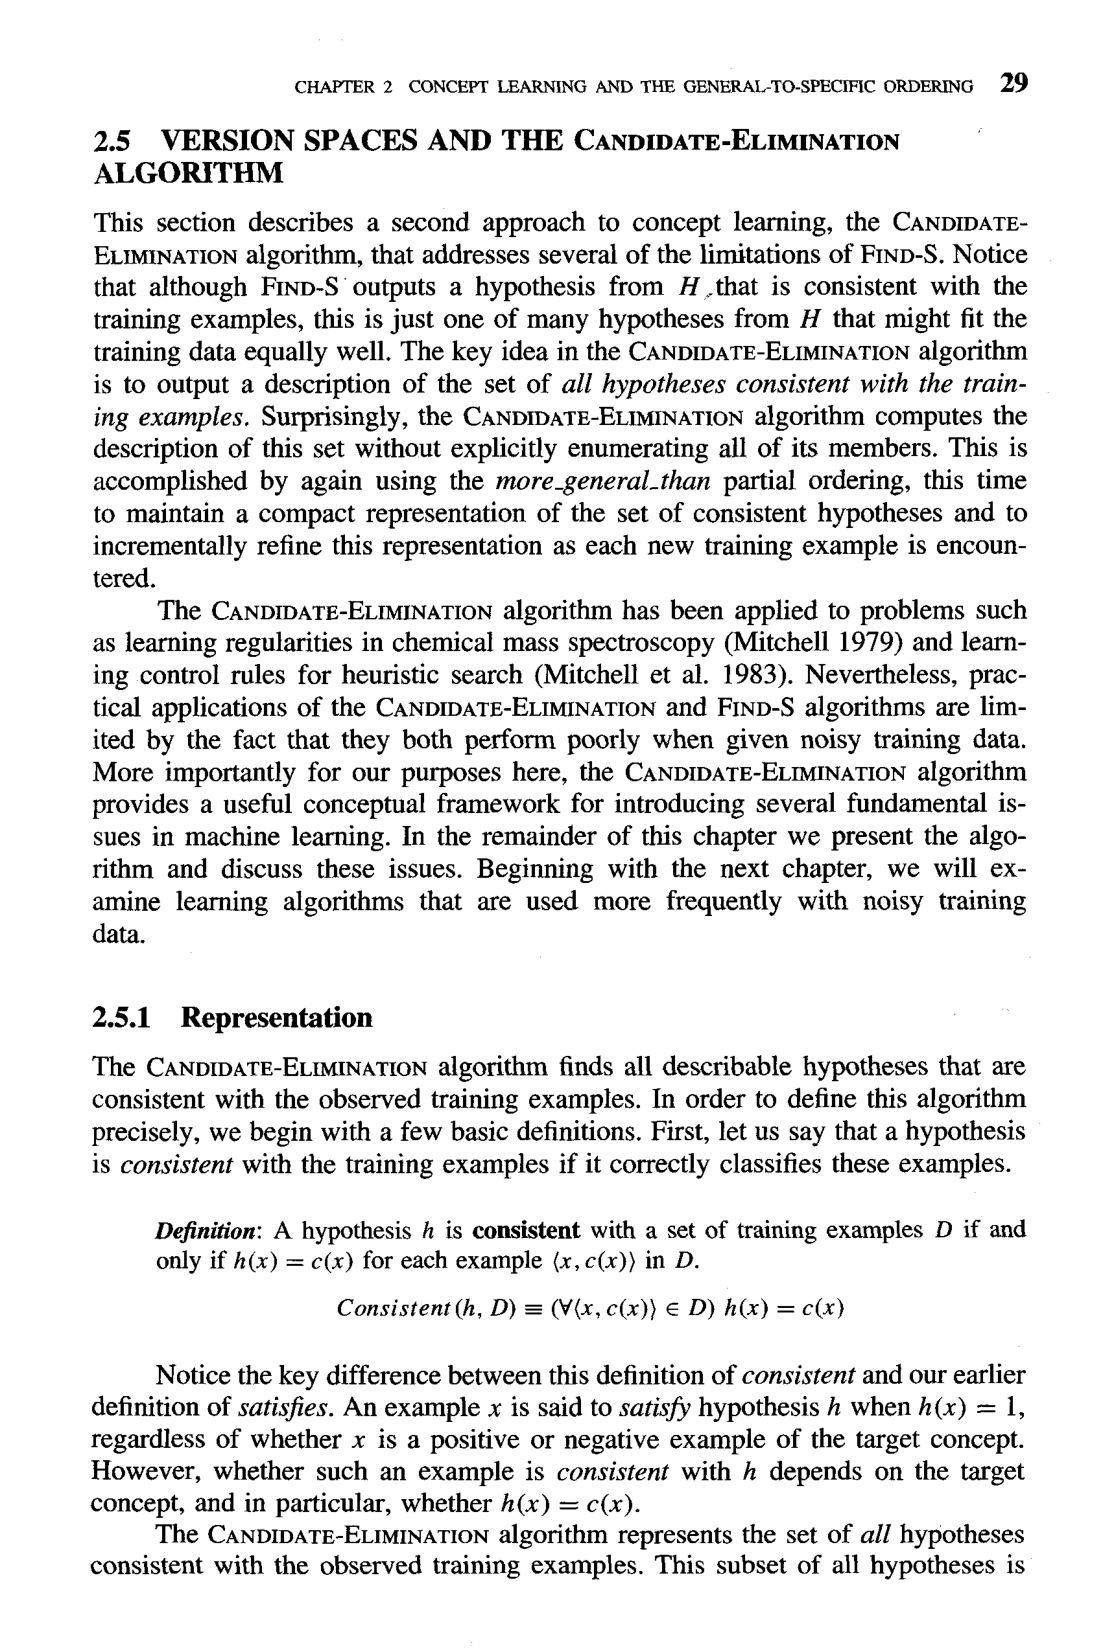
\includegraphics[width=0.9\linewidth]{figures/p41_b0.png}
\end{figure}

\subsection{VERSION SPACES AND THE CANDIDATE-ELIMINATION ALGORITHM}

Phần này mô tả cách tiếp cận thứ hai đối với concept learning, thuật toán CANDIDATEELIMINATION, nhằm giải quyết một số hạn chế của FIND-S. Để ý

Rằng mặc dù FIND-S đưa ra giả thuyết từ H, điều đó nhất quán với các ví dụ training, nhưng đây chỉ là một trong nhiều giả thuyết từ H có thể phù hợp tốt như nhau với dữ liệu training. Ý tưởng chính trong thuật toán CANDIDATE-ELIMINATION

Là đưa ra mô tả về tập hợp tất cả các giả thuyết phù hợp với các ví dụ training. Điều đáng ngạc nhiên là thuật toán CANDIDATE-ELIMINATION tính toán

Mô tả tập hợp này mà không liệt kê rõ ràng tất cả các thành viên của nó. Điều này được thực hiện bằng cách sử dụng thứ tự tổng quát hơn từng phần, lần này để duy trì cách biểu diễn nhỏ gọn của tập hợp các giả thuyết nhất quán và tinh chỉnh dần cách biểu diễn này khi gặp mỗi ví dụ training mới.

\subsection{Thuật toán CANDIDATE-ELIMINATION đã được áp dụng cho các bài toán như}

Như học các quy tắc trong quang phổ khối hóa học (Mitchell 1979) và học các quy tắc kiểm soát cho tìm kiếm heuristic (Mitchell và cộng sự 1983). Tuy nhiên, các ứng dụng thực tế của thuật toán CANDIDATE-ELIMINATION và FIND-S còn hạn chế.

Thực tế là cả hai đều hoạt động kém khi được cung cấp dữ liệu training ồn ào. Quan trọng hơn cho mục đích của chúng ta ở đây, thuật toán CANDIDATE-ELIMINATION

Cung cấp một khung khái niệm hữu ích để giới thiệu một số vấn đề cơ bản-

Kiện machine learning. Trong phần còn lại của chương này chúng ta trình bày thuật toán

Nhịp điệu và thảo luận về những vấn đề này. Bắt đầu với chương tiếp theo, chúng ta sẽ xem xét các thuật toán học được sử dụng thường xuyên hơn với dữ liệu training nhiễu.

\subsubsection{Biểu diễn}

Thuật toán CANDIDATE-ELIMINATION tìm thấy tất cả các giả thuyết có thể mô tả được

Phù hợp với các ví dụ training được quan sát. Để định nghĩa thuật toán này một cách chính xác, chúng ta bắt đầu với một vài định nghĩa cơ bản. Đầu tiên, chúng ta hãy nói rằng một giả thuyết phù hợp với các ví dụ training nếu nó classification chính xác các ví dụ này.

Định nghĩa: Giả thuyết h phù hợp với tập hợp các ví dụ training D nếu và

\[only if h(x) = c(x) for each example (x, c(x)) in D.\]

Lưu ý sự khác biệt chính giữa định nghĩa nhất quán này và định nghĩa trước đó của chúng ta.

Định nghĩa về thỏa mãn Một ví dụ x được cho là thỏa mãn giả thuyết h khi h(x) = 1, bất kể x là ví dụ tích cực hay tiêu cực của khái niệm mục tiêu. Tuy nhiên, liệu một ví dụ như vậy có nhất quán với h hay không còn phụ thuộc vào khái niệm mục tiêu và cụ thể là liệu h(x) = c(x) hay không.

Thuật toán CANDIDATE-ELIMINATION đại diện cho tập hợp tất cả các giả thuyết

Phù hợp với các ví dụ training được quan sát. Tập hợp con của tất cả các giả thuyết này là

% --- page 42 ---
\begin{figure}[ht]
\centering

\includegraphics[width=0.9\linewidth]{figures/p42_b0.png}
\end{figure}

Được gọi là version space đối với hypothesis space H và các ví dụ training D, vì nó chứa tất cả các phiên bản hợp lý của khái niệm mục tiêu.

Xác định: version space, ký hiệu là VSHVD, đối với hypothesis space H

Và các mẫu training D, là tập con các giả thuyết từ H phù hợp với các mẫu training trong D.

V S H , \textasciitilde{} = \{h E HIConsistent(h, D)]

\subsubsection{Thuật toán LIST-THEN-ELIMINATE}

Một cách rõ ràng để thể hiện version space chỉ đơn giản là liệt kê tất cả các thành viên của nó. Điều này dẫn đến một thuật toán học đơn giản mà chúng ta có thể gọi là thuật toán LIST-THENELIMINATE, được xác định trong Bảng 2.4.

Thuật toán LIST-THEN-ELIMINATE trước tiên khởi tạo version space để điều khiển

Thu được tất cả các giả thuyết trong H, sau đó loại bỏ bất kỳ giả thuyết nào được tìm thấy không nhất quán với bất kỳ ví dụ training nào. Do đó, version space của các giả thuyết ứng cử viên sẽ co lại khi quan sát được nhiều ví dụ hơn, cho đến khi lý tưởng nhất là chỉ còn lại một giả thuyết phù hợp với tất cả các ví dụ được quan sát. Đây có lẽ là khái niệm mục tiêu mong muốn. Nếu không có đủ dữ liệu để thu hẹp version space thành một giả thuyết duy nhất thì thuật toán có thể đưa ra toàn bộ tập hợp giả thuyết phù hợp với dữ liệu được quan sát.

Về nguyên tắc, thuật toán LIST-THEN-ELIMINATE có thể được áp dụng bất cứ khi nào

Hypothesis space H là hữu hạn. Nó có nhiều ưu điểm, bao gồm cả việc đảm bảo đưa ra tất cả các giả thuyết phù hợp với dữ liệu training. Thật không may, nó đòi hỏi phải liệt kê đầy đủ tất cả các giả thuyết trong H-an không thực tế.

Yêu cầu cho tất cả trừ hypothesis spaces tầm thường nhất.

\subsubsection{Một cách biểu diễn nhỏ gọn hơn cho Version Spaces}

Thuật toán CANDIDATE-ELIMINATION hoạt động theo nguyên tắc tương tự như trên

Thuật toán LIST-THEN-ELIMINATE. Tuy nhiên, nó sử dụng một đại diện nhỏ gọn hơn nhiều.

Sự phẫn nộ của version space. Đặc biệt, version space được đại diện bởi các thành viên chung nhất và ít chung nhất. Các thành viên này hình thành chung và

Các bộ ranh giới cụ thể phân định version space trong phạm vi được sắp xếp một phần

Hypothesis space.

\subsection{Thuật toán LIST-THEN-ELIMINATE}

1. VersionSpace c danh sách chứa mọi giả thuyết trong H

2. Với mỗi ví dụ training, (x, c(x))

Loại bỏ khỏi VersionSpace mọi giả thuyết h mà h(x) \# c(x)

3. Xuất danh sách giả thuyết vào VersionSpace

\noindent\textit{TABLE 2.4 Thuật toán LIST-THEN-ELIMINATE.}

% --- page 43 ---
\begin{figure}[ht]
\centering
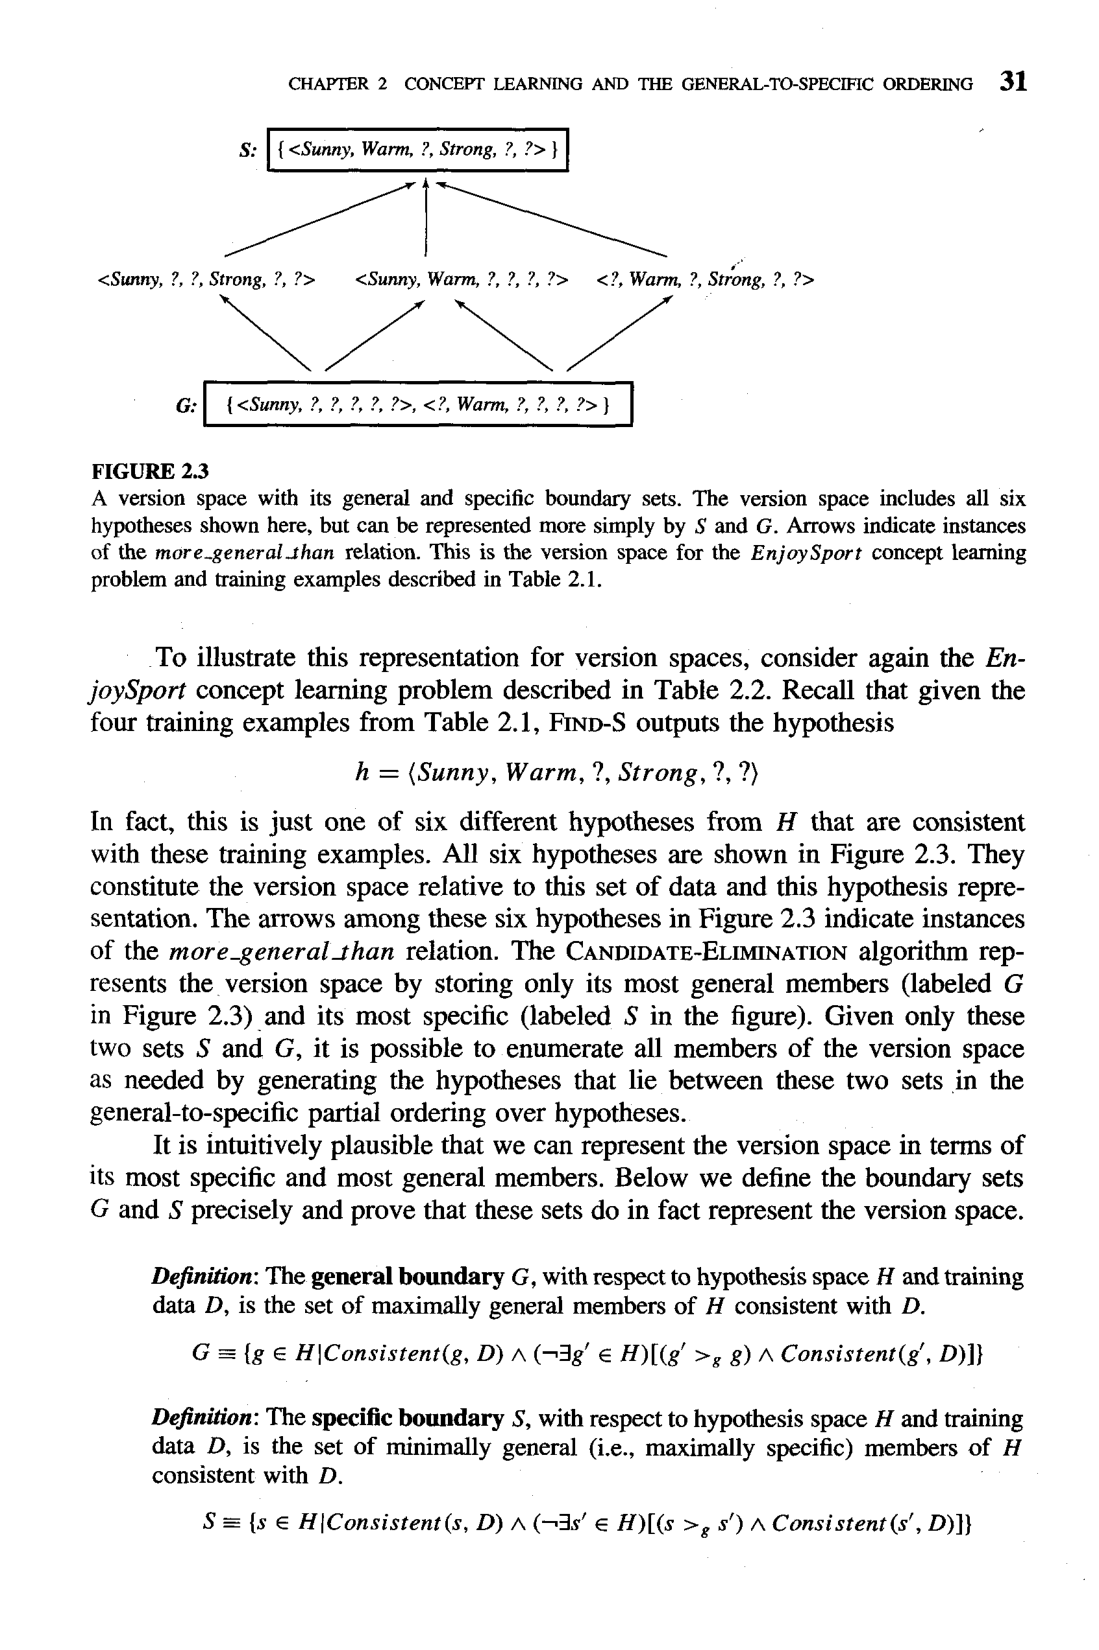
\includegraphics[width=0.9\linewidth]{figures/p43_b0.png}
\end{figure}

\{<Nắng, Ấm áp, ?, Mạnh mẽ, 7, ?> 1

<Nắng, ?, 7, Mạnh mẽ, 7, ?> <Nắng, Ấm áp, ?. ?, ?, ?> <?, Ấm áp, ?, strbng, ?, ?>

\noindent\textit{FIGURE 2.3 A version space với các bộ ranh giới chung và cụ thể. Version space bao gồm tất cả sáu giả thuyết được trình bày ở đây, nhưng có thể được biểu diễn đơn giản hơn bằng S và G. Các mũi tên chỉ ra các trường hợp của mối quan hệ tổng quát hơn. Đây là version space dành cho bài tập Enjoysport concept learning và các ví dụ training được mô tả trong Bảng 2.1.}

Để minh họa cách biểu diễn này cho version spaces, hãy xem xét lại En-

Bài toán joysport concept learning được mô tả ở Bảng 2.2. Hãy nhớ lại rằng đã đưa ra

Bốn ví dụ training từ Bảng 2.1, FIND-S đưa ra giả thuyết

H = (Nắng, Ấm áp, ?, Mạnh mẽ, ?, ?)

Trên thực tế, đây chỉ là một trong sáu giả thuyết khác với H phù hợp với các ví dụ training này. Tất cả sáu giả thuyết được trình bày trong Hình 2.3. Chúng tạo thành version space liên quan đến dataset này và cách trình bày giả thuyết này. Các mũi tên trong số sáu giả thuyết này ở Hình 2.3 chỉ ra những trường hợp của mối quan hệ han tổng quát hơn. Đại diện thuật toán CANDIDATE-ELIMINATION

Bực bội với version space bằng cách chỉ lưu trữ các thành viên chung nhất của nó (được gắn nhãn G trong Hình 2.3) và cụ thể nhất của nó (được gắn nhãn S trong hình). Chỉ với hai bộ S và G này, có thể liệt kê tất cả các thành viên của version space khi cần bằng cách tạo ra các giả thuyết nằm giữa hai bộ này theo thứ tự từng phần từ tổng quát đến cụ thể trên các giả thuyết.

Về mặt trực quan, có vẻ hợp lý khi chúng ta có thể biểu diễn version space theo

Thành viên cụ thể nhất và tổng quát nhất của nó. Dưới đây chúng ta xác định các bộ ranh giới

G và S một cách chính xác và chứng minh rằng các bộ này trên thực tế đại diện cho version space.

Định nghĩa: Ranh giới chung G đối với hypothesis space H và training

Dữ liệu D, là tập hợp các phần tử tổng quát lớn nhất của H phù hợp với D.

G = \{g E HIConsistent(g, D) A (-3gf E H)[(gf >, g) A Nhất quán(gt, D)]]

Định nghĩa: Ranh giới cụ thể S đối với hypothesis space H và training

Dữ liệu D, là tập hợp các thành viên tổng quát tối thiểu (nghĩa là cụ thể tối đa) của H phù hợp với D.

S rn \{s E H(Nhất quán(s, D) A (-3s' E H)[(s >, sf) A Nhất quán(st, D)])

% --- page 44 ---
\begin{figure}[ht]
\centering
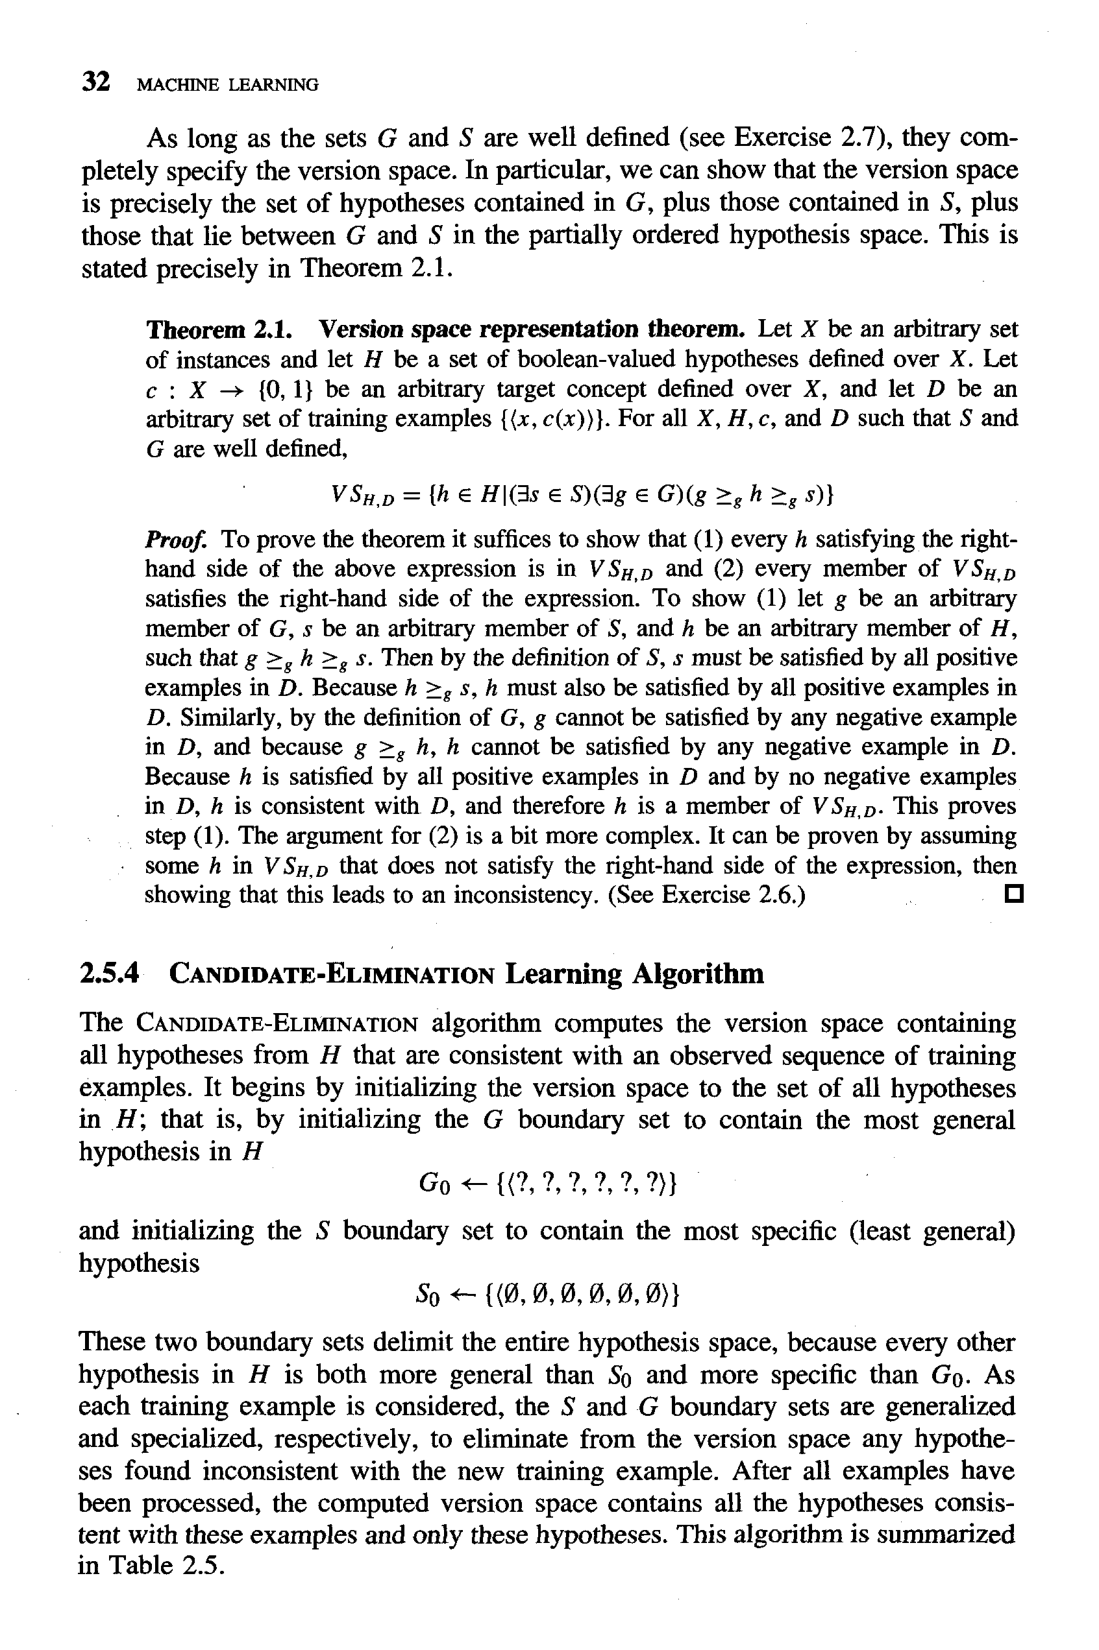
\includegraphics[width=0.9\linewidth]{figures/p44_b0.png}
\end{figure}

Miễn là các tập G và S được xác định rõ ràng (xem Bài tập 2.7), chúng sẽ

Chỉ định đầy đủ version space. Cụ thể, chúng ta có thể chỉ ra rằng version space chính xác là tập hợp các giả thuyết chứa trong G, cộng với các giả thuyết chứa trong S, cộng với các giả thuyết nằm giữa G và S trong hypothesis space được sắp thứ tự một phần. Điều này được phát biểu chính xác trong Định lý 2.1.

Định lý 2.1. Định lý biểu diễn Version space. Đặt X là một tập hợp các trường hợp tùy ý và đặt H là một tập hợp các giả thuyết có giá trị boolean được xác định trên X. Đặt c : X + \{O, 1) là một khái niệm mục tiêu tùy ý được xác định trên X và đặt D là một tập hợp các ví dụ training tùy ý \{(x, c(x))). Với mọi X, H, c và D sao cho S và G được xác định rõ,

Bằng chứng. Để chứng minh định lý chỉ cần chỉ ra rằng (1) mọi h thỏa mãn vế phải của biểu thức trên đều thuộc V S H , \textasciitilde{} và (2) mọi thành viên của V S H , \textasciitilde{}

Thỏa mãn vế phải của biểu thức. Chứng minh (1) cho g là thành viên tùy ý của G, s là thành viên tùy ý của S, và h là thành viên tùy ý của H, sao cho g 2, h 2, s. Khi đó theo định nghĩa của S, s phải thỏa mãn mọi ví dụ dương trong D. Vì h 2, s, h cũng phải thỏa mãn mọi ví dụ dương trong

D. Tương tự, theo định nghĩa của G, g không thể được thỏa mãn bởi bất kỳ ví dụ phủ định nào

Trong D, và vì g 2, h, h không thể được thỏa mãn bởi bất kỳ ví dụ phủ định nào trong D. Bởi vì h được thỏa mãn bởi tất cả các ví dụ phủ định trong D và không có ví dụ phủ định nào trong D, nên h phù hợp với D, và do đó h là thành viên của V S H , \textasciitilde{} . Điều này chứng tỏ

Bước (1). Lập luận cho (2) phức tạp hơn một chút. Nó có thể được chứng minh bằng cách giả sử một số h trong V S H , \textasciitilde{} không thỏa mãn vế phải của biểu thức, thì

Cho thấy điều này dẫn đến sự không nhất quán. (Xem Bài tập 2.6.) 0

\subsubsection{Thuật toán học CANDIDATE-ELIMINATION}

Thuật toán CANDIDATE-ELIMINATION tính toán version space chứa

Tất cả các giả thuyết từ H phù hợp với chuỗi các ví dụ training được quan sát. Nó bắt đầu bằng việc khởi tạo version space thành tập hợp tất cả các giả thuyết trong H; nghĩa là, bằng cách khởi tạo tập ranh giới G để chứa giả thuyết tổng quát nhất trong H

Đi + \{(?, ?, ?, ?, ?, ?)\}

Và khởi tạo tập ranh giới S để chứa giả thuyết cụ thể nhất (ít tổng quát nhất)

Vậy c- ((@,PI, @,PI, 0,0)1

Hai tập hợp ranh giới này phân định toàn bộ hypothesis space, bởi vì mọi giả thuyết khác trong H đều tổng quát hơn So và cụ thể hơn Go. Khi mỗi mẫu training được xem xét, các tập ranh giới S và G lần lượt được tổng quát hóa và chuyên biệt hóa để loại bỏ khỏi version space bất kỳ giả thuyết nào được cho là không nhất quán với mẫu training mới. Sau khi tất cả các ví dụ có

Được xử lý, version space được tính toán chứa tất cả các giả thuyết phù hợp với các ví dụ này và chỉ những giả thuyết này. Thuật toán này được tóm tắt trong Bảng 2.5.

% --- page 45 ---
\begin{figure}[ht]
\centering
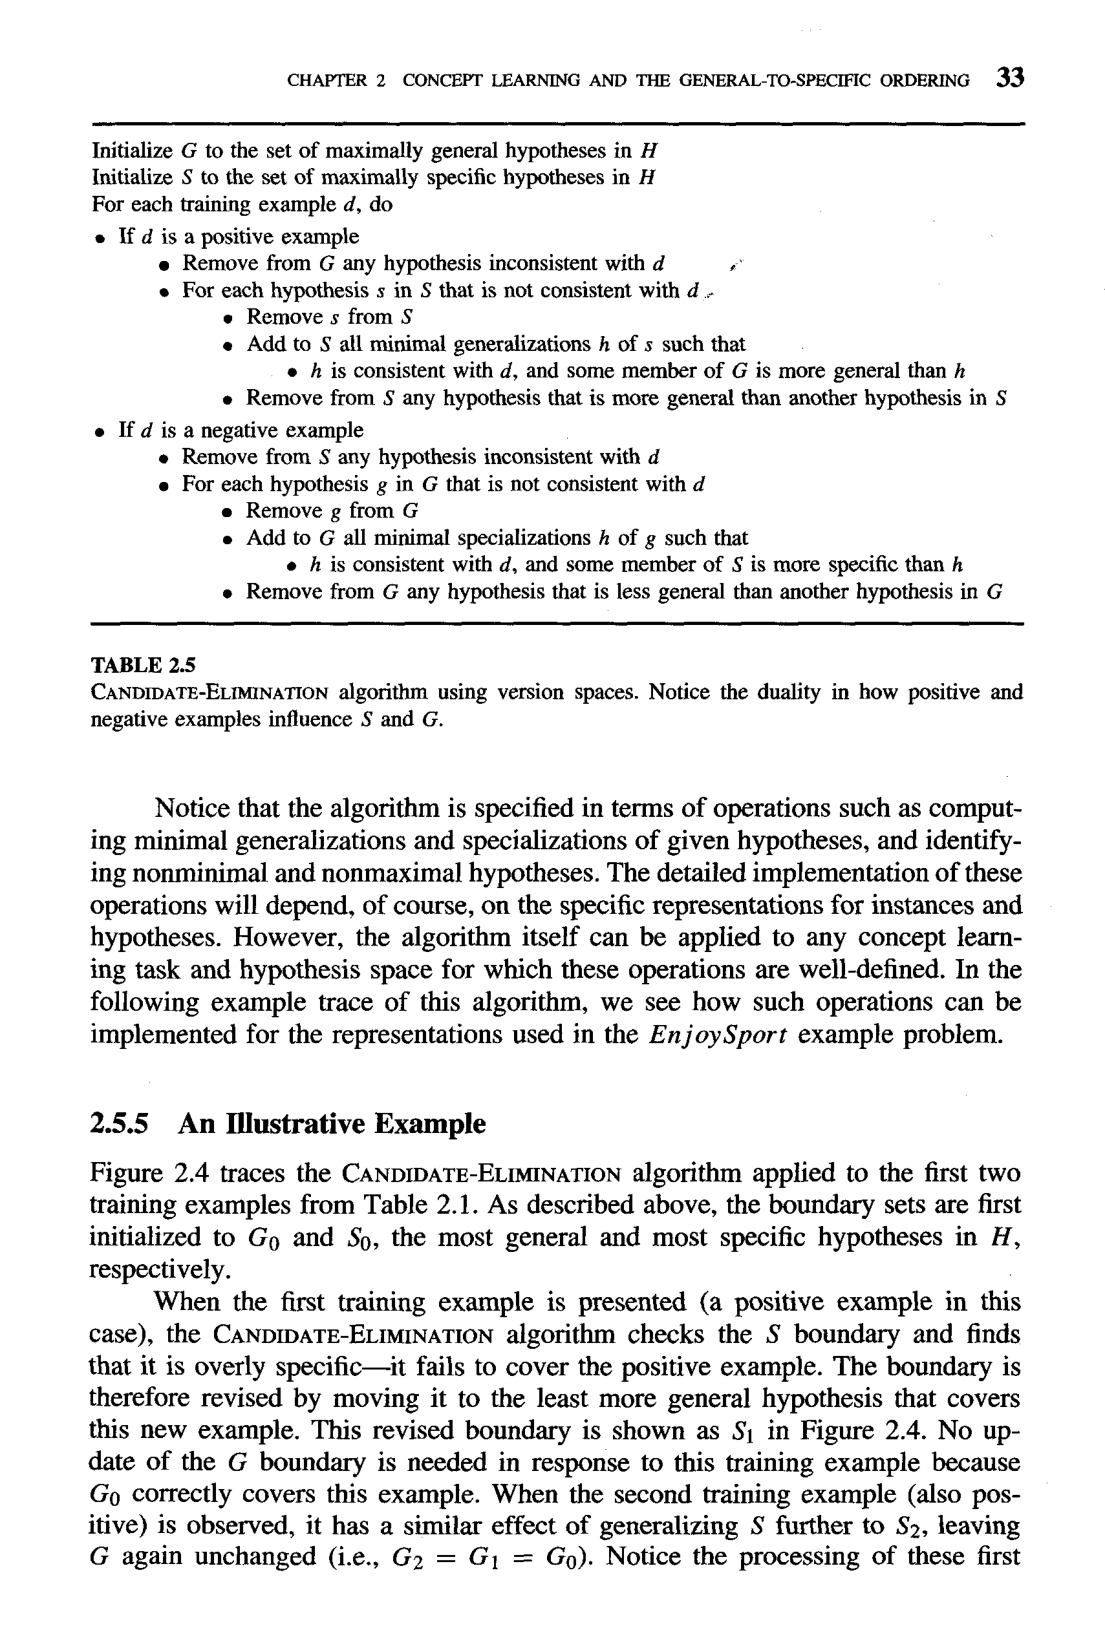
\includegraphics[width=0.9\linewidth]{figures/p45_b0.png}
\end{figure}

\subsection{CHAPTER 2 CONCEET LEARNJNG AND THE GENERAL-TO-SPECIFIC ORDERING 33}

Khởi tạo G thành tập giả thuyết tổng quát tối đa trong H Khởi tạo S thành tập giả thuyết cụ thể tối đa trong H Với mỗi ví dụ training d, hãy thực hiện

\section{Nếu d là một ví dụ tích cực}

\subsection{Loại bỏ khỏi G mọi giả thuyết không nhất quán với d ,}

\section{Với mỗi giả thuyết s trong S không phù hợp với d ,-}

\section{Xóa s khỏi S}

\section{Thêm vào S tất cả các tổng quát hóa tối thiểu h của s sao cho}

\section{h phù hợp với d và một số thành viên của G tổng quát hơn h}

\section{Loại bỏ khỏi S bất kỳ giả thuyết nào tổng quát hơn giả thuyết khác trong S}

\section{Nếu d là một ví dụ tiêu cực}

\section{Loại bỏ khỏi S mọi giả thuyết không nhất quán với d}

Với mỗi giả thuyết g trong G không phù hợp với d

Xóa g khỏi G

\section{Thêm vào G tất cả các chuyên môn tối thiểu h của g sao cho}

\section{h phù hợp với d và một số thành viên của S cụ thể hơn h}

\section{Loại bỏ khỏi G bất kỳ giả thuyết nào ít tổng quát hơn giả thuyết khác trong G}

\noindent\textit{Thuật toán TABLE 2.5 CANDIDATE-ELIMINATION sử dụng version spaces. Lưu ý tính hai mặt trong mức độ tích cực và}

Ví dụ tiêu cực ảnh hưởng đến S và G.

Lưu ý rằng thuật toán được chỉ định dưới dạng các hoạt động như tính toán

Khái quát hóa và chuyên biệt hóa tối thiểu các giả thuyết đã cho, đồng thời xác định các giả thuyết không tối thiểu và không tối đa. Tất nhiên, việc triển khai chi tiết các thao tác này sẽ phụ thuộc vào cách biểu diễn cụ thể cho các trường hợp và giả thuyết. Tuy nhiên, bản thân thuật toán có thể được áp dụng cho bất kỳ tác vụ concept learning nào và hypothesis space nào mà các hoạt động này được xác định rõ ràng. Trong dấu vết ví dụ sau đây của thuật toán này, chúng ta thấy cách các hoạt động như vậy có thể được triển khai cho các biểu diễn được sử dụng trong bài toán ví dụ EnjoySport.

\subsubsection{Một ví dụ minh họa}

\noindent\textit{Hình 2.4 theo dõi thuật toán CANDIDATE-ELIMINATION được áp dụng cho hai thuật toán đầu tiên}

Ví dụ training từ Bảng 2.1. Như đã mô tả ở trên, các tập ranh giới trước tiên được khởi tạo thành Go và So, tương ứng là các giả thuyết tổng quát nhất và cụ thể nhất trong H.

Khi ví dụ training đầu tiên được trình bày (một ví dụ tích cực trong phần này

Trường hợp), thuật toán CANDIDATE-ELIMINATION kiểm tra ranh giới S và tìm thấy

Rằng nó quá cụ thể - nó không bao gồm được ví dụ tích cực. Ranh giới là

Do đó được sửa đổi bằng cách chuyển nó sang giả thuyết ít tổng quát hơn bao gồm ví dụ mới này. Ranh giới sửa đổi này được hiển thị dưới dạng S1 trong Hình 2.4. Không cần cập nhật ranh giới G trong response cho ví dụ training này vì

Go bao gồm chính xác ví dụ này. Khi ví dụ training thứ hai (cũng có thể

Itive) được quan sát thấy, nó có tác dụng tương tự trong việc khái quát hóa S hơn nữa thành S2, để lại

\[G again unchanged (i.e., G2 = GI = GO). Notice the processing of these first\]

% --- page 46 ---
\begin{figure}[ht]
\centering

\includegraphics[width=0.9\linewidth]{figures/p46_b0.png}
\end{figure}

\section{MACHINE LEARNING}

S 1 : \{<Nắng, Ấm áp, Bình thường, Mạnh mẽ, Ấm áp, Giống nhau> \} 1

Ví dụ training:

T

\section{. <Nắng, Ấm áp, Bình thường, Khỏe mạnh, Ấm áp, Tương tự>, Thích thể thao = Có}

\section{. <Nắng, Ấm, Cao, Mạnh mẽ, Ấm áp, Giống nhau>, Thích thể thao = Có}

S2:

\noindent\textit{FIGURE 2.4 CANDIDATE-ELIMINATION Trace 1. So và Go là các tập ranh giới ban đầu tương ứng với nhiều nhất}

Giả thuyết cụ thể và tổng quát nhất. Ví dụ training 1 và 2 buộc ranh giới S trở nên tổng quát hơn, như trong thuật toán FIND-S. Chúng không có tác dụng lên ranh giới G.

\{<Nắng, Ấm áp, ?, Mạnh mẽ, Ấm áp, Giống nhau>\}

Hai ví dụ tích cực rất giống với quá trình xử lý được thực hiện bởi thuật toán FIND-S.

Như được minh họa bằng hai bước đầu tiên này, các ví dụ training tích cực có thể buộc

Ranh giới S của version space ngày càng trở nên chung chung. Các ví dụ training phủ định đóng vai trò bổ sung trong việc buộc ranh giới G ngày càng trở nên cụ thể. Hãy xem xét ví dụ training thứ ba, được hiển thị trong Hình 2.5. Ví dụ tiêu cực này cho thấy ranh giới G của version space là quá chung chung; tức là giả thuyết trong G dự đoán sai rằng ví dụ mới này là một ví dụ tích cực. Do đó, giả thuyết trong ranh giới G phải được chuyên biệt hóa cho đến khi nó classification chính xác ví dụ phủ định mới này. Như được hiển thị trong Hình 2.5, có một số giả thuyết thay thế cụ thể hơn ở mức tối thiểu. Tất cả những thứ này đều trở thành thành viên của bộ ranh giới G3 mới. -

Cho rằng có sáu thuộc tính có thể được chỉ định để chuyên hóa G2,

Tại sao chỉ có ba giả thuyết mới trong G3? Ví dụ: giả thuyết h = (?, ?, Bình thường, ?, ?, ?) là một chuyên môn hóa tối thiểu của G2 gắn nhãn chính xác cho ví dụ mới là ví dụ phủ định, nhưng nó không được đưa vào Gg. Lý do giả thuyết này bị loại trừ là vì nó không phù hợp với các ví dụ tích cực đã gặp trước đó. Thuật toán xác định điều này một cách đơn giản bằng cách lưu ý rằng h không tổng quát hơn ranh giới cụ thể hiện tại, Sz. Trên thực tế, ranh giới S của version space tạo thành một bản tóm tắt các ví dụ tích cực đã gặp trước đó có thể được sử dụng để xác định liệu có bất kỳ giả thuyết nào được đưa ra hay không.

% --- page 47 ---
\begin{figure}[ht]
\centering

\includegraphics[width=0.9\linewidth]{figures/p47_b0.png}
\end{figure}

C H m R 2 CONCEPT LEARNING AND THE GENERAL-TO-SPECIFIC ORDERING 35

S2 9 giây 3 :

Ví dụ training:

( <Sunny, Wann, ?. Strong, Warn Same> )]

G 3:

3. <Mưa, Lạnh, Cao, Mạnh, Ấm, Thay đổi>, EnjoySporkNo

(<Sunny, ?, ?, ?, ?, ?> <?, Wann, ?, ?, ?, ?> <?, ?, ?, ?, ?, Tương tự>\}

\noindent\textit{FIGURE 2.5 CANDIDATE-ELMNATION Dấu vết 2. Ví dụ training 3 là một ví dụ tiêu cực buộc G2}

Ranh giới được chuyên biệt hóa cho G3. Lưu ý một số giả thuyết tổng quát tối đa thay thế được đưa vào Gj.

Phù hợp với những ví dụ này. Theo định nghĩa, bất kỳ giả thuyết nào tổng quát hơn S sẽ bao trùm mọi ví dụ mà S đề cập và do đó sẽ bao hàm mọi ví dụ tích cực trong quá khứ. Theo kiểu kép, ranh giới G tóm tắt thông tin từ các ví dụ tiêu cực gặp phải trước đó. Bất kỳ giả thuyết nào cụ thể hơn G đều được đảm bảo phù hợp với các ví dụ tiêu cực trong quá khứ. Điều này đúng vì bất kỳ giả thuyết nào như vậy, theo định nghĩa, không thể bao hàm các ví dụ mà G không bao hàm.

Ví dụ training thứ tư, như trong Hình 2.6, khái quát hơn nữa về

Ranh giới S của version space. Nó cũng dẫn đến việc loại bỏ một thành viên của G

Ranh giới, bởi vì thành viên này không bao gồm được ví dụ tích cực mới. Hành động cuối cùng này là kết quả của bước đầu tiên với điều kiện "Nếu d là một ví dụ tích cực" trong thuật toán được trình bày trong Bảng 2.5. Để hiểu cơ sở lý luận của bước này, sẽ rất hữu ích khi xem xét lý do tại sao giả thuyết vi phạm phải được loại bỏ khỏi G. Lưu ý rằng nó không thể chuyên biệt hóa, bởi vì việc chuyên môn hóa nó sẽ không làm cho nó bao trùm được ví dụ mới. Nó cũng không thể được khái quát hóa, bởi vì theo định nghĩa của G, bất kỳ giả thuyết tổng quát nào cũng sẽ bao hàm ít nhất một ví dụ training phủ định. Do đó, giả thuyết phải được loại bỏ khỏi ranh giới G, do đó loại bỏ toàn bộ một nhánh của trật tự một phần khỏi version space của các giả thuyết còn lại đang được xem xét.

Sau khi xử lý bốn ví dụ này, ranh giới đặt giới hạn S4 và G4

Version space của tất cả các giả thuyết phù hợp với tập hợp các ví dụ training được quan sát tăng dần. Toàn bộ version space, bao gồm cả những giả thuyết đó

MỘT

'32: Tôi<?, ?, ?, ?, ?,?>Tôi

% --- page 48 ---
\begin{figure}[ht]
\centering
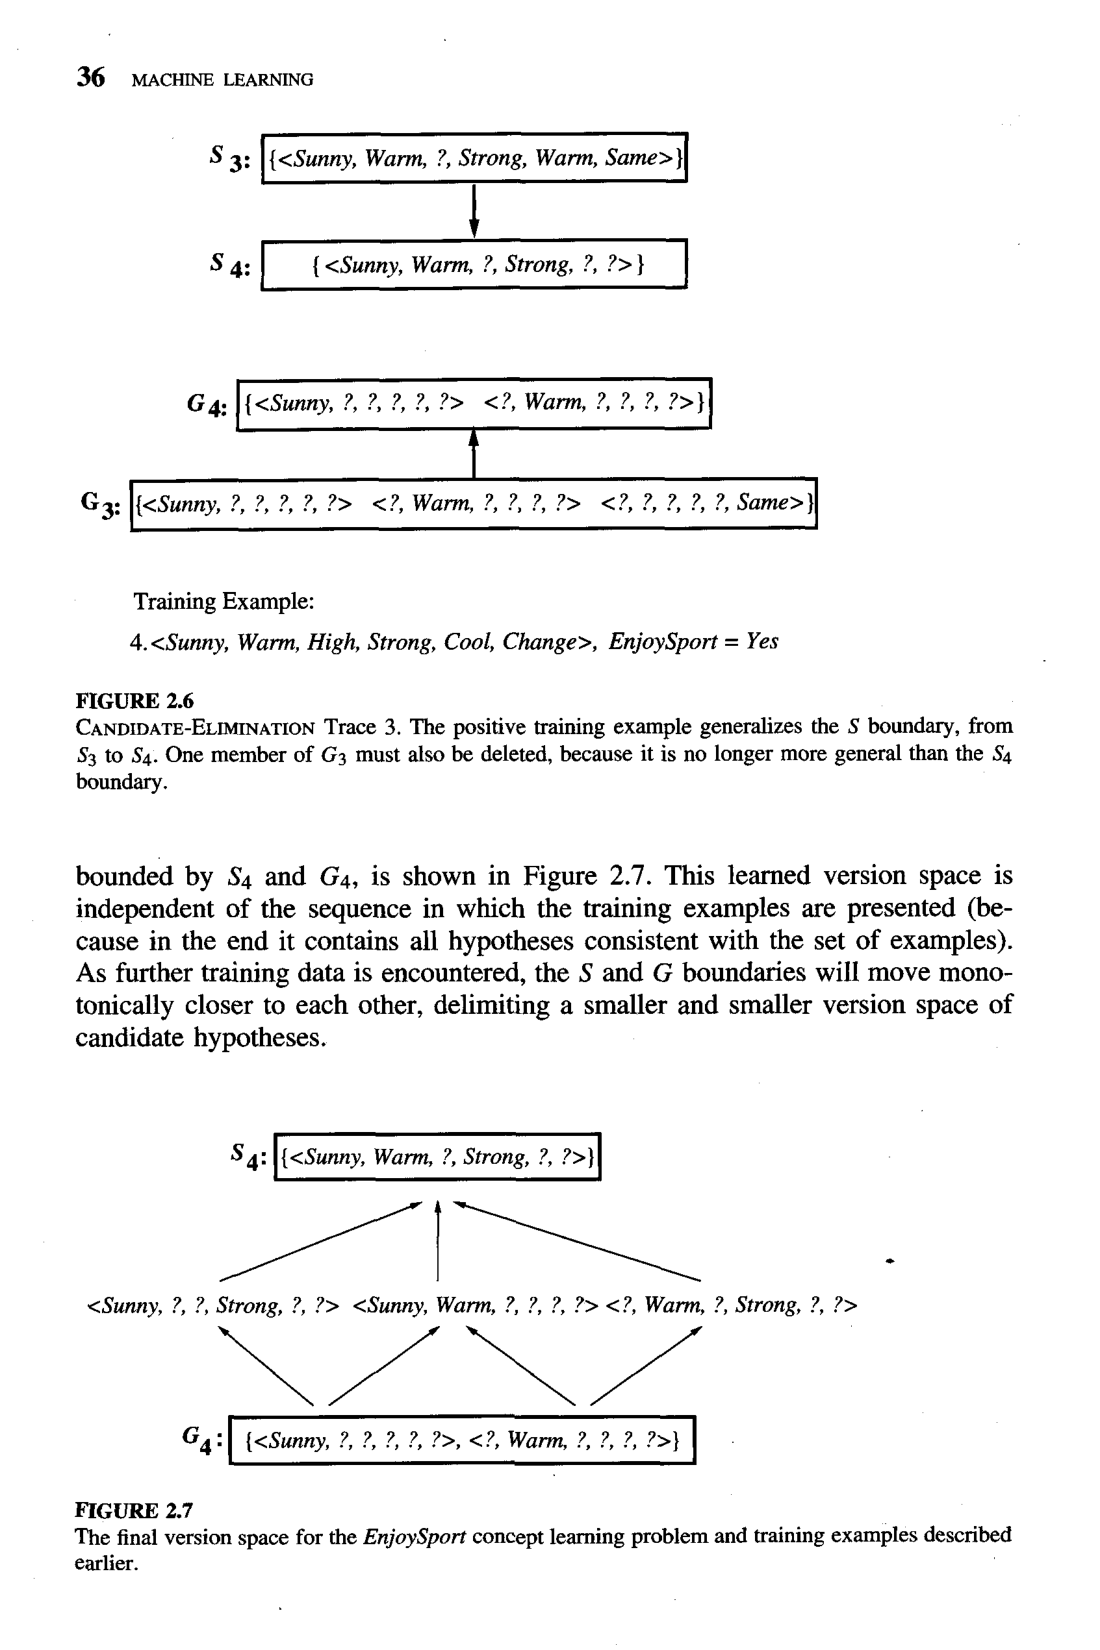
\includegraphics[width=0.9\linewidth]{figures/p48_b0.png}
\end{figure}

S 3: \{<Nắng, Ấm áp, ?, Mạnh mẽ, Ấm áp, Tương tự>)

TÔI

S 4: Tôi ( <Nắng, Ấm áp ?, Mạnh mẽ, ?, ?> ) Tôi

Ví dụ training:

4. <Nắng, Ấm áp, Cao, Mạnh mẽ, Mát mẻ, Thay đổi>, EnjoySport = Có

\noindent\textit{FIGURE 2.6 CANDIDATE-ELIMINATION Trace 3. Ví dụ training tích cực khái quát hóa ranh giới S, từ}

S3 đến S4. Một thành viên của Gg cũng phải bị xóa vì nó không còn chung chung hơn S4

Ranh giới.

Giới hạn bởi S4 và G4, được minh họa trong Hình 2.7. Version space đã học này độc lập với trình tự trình bày các ví dụ training (vì cuối cùng nó chứa tất cả các giả thuyết phù hợp với tập hợp các ví dụ). Khi gặp thêm dữ liệu training, ranh giới S và G sẽ di chuyển đơn điệu đến gần nhau hơn, phân định version space ngày càng nhỏ hơn trong các giả thuyết ứng cử viên.

<Nắng, ?, ?, Mạnh mẽ, ?, ?> <Nắng, Ấm áp, ?, ?, ?, ?> <?, Ấm áp, ?, Mạnh mẽ, ?, ?>

S4:

\{<Nắng, ?, ?, ?, ?, ?>, <?, Ấm áp, ?, ?, ?, ?>)

\{<Nắng, Ấm áp, ?, Mạnh mẽ, ?, ?>)

\noindent\textit{FIGURE 2.7 version space cuối cùng cho bài toán EnjoySport concept learning và các ví dụ training được mô tả trước đó.}

% --- page 49 ---
\begin{figure}[ht]
\centering
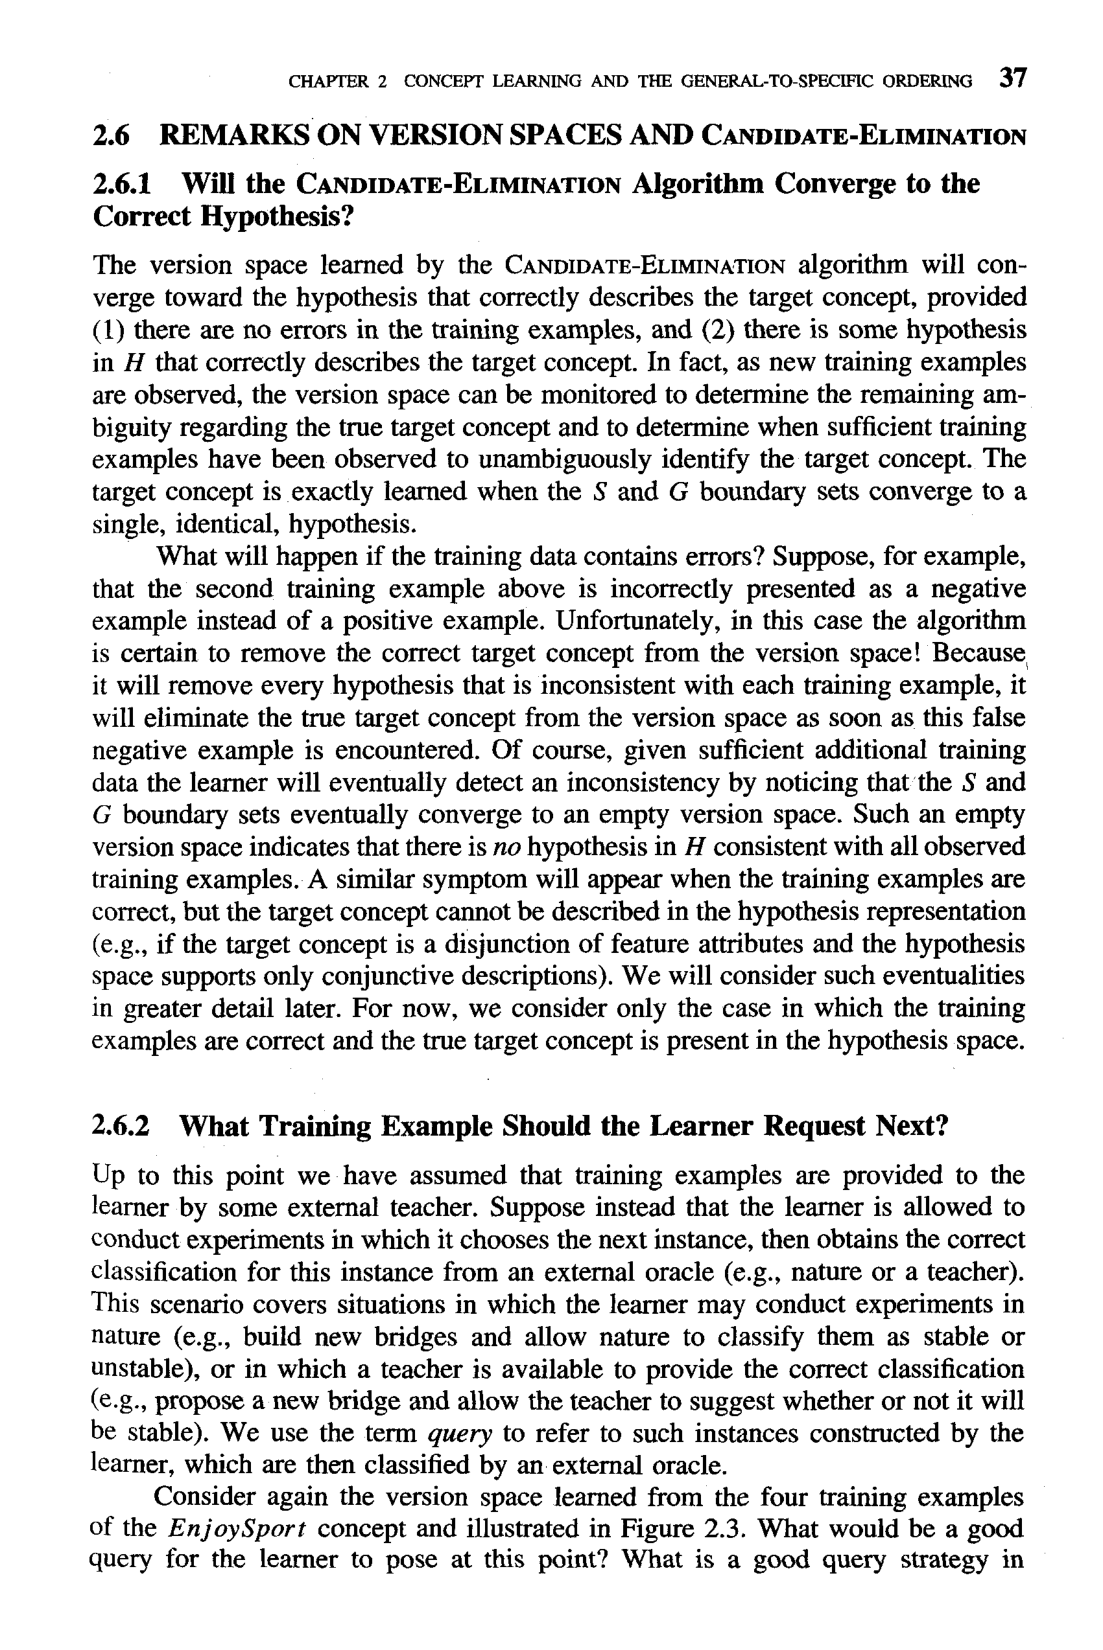
\includegraphics[width=0.9\linewidth]{figures/p49_b0.png}
\end{figure}

CH.4PTF.R 2 CONCEFT LEARNING AND THE GENERAL-TO-SPECIFIC ORDERING 37

\subsection{REMARKS ON VERSION SPACES AND CANDIDATE-ELIMINATION}

\subsubsection{Thuật toán CANDIDATE-ELIMINATION có hội tụ về}

Giả thuyết đúng?

Version space được học bằng thuật toán CANDIDATE-ELIMINATION sẽ

Hướng tới giả thuyết mô tả chính xác khái niệm mục tiêu, với điều kiện (1) không có lỗi trong các ví dụ training và (2) có một số giả thuyết trong H mô tả chính xác khái niệm mục tiêu. Trên thực tế, khi quan sát các mẫu training mới, version space có thể được theo dõi để xác định sự mơ hồ còn lại liên quan đến khái niệm mục tiêu thực sự và để xác định khi nào đã quan sát đủ các mẫu training để xác định rõ ràng khái niệm mục tiêu. Khái niệm mục tiêu được học chính xác khi các tập ranh giới S và G hội tụ về một giả thuyết duy nhất, giống hệt nhau.

Điều gì sẽ xảy ra nếu dữ liệu training có lỗi? Giả sử, ví dụ,

Rằng ví dụ training thứ hai ở trên được trình bày không chính xác dưới dạng ví dụ tiêu cực thay vì ví dụ tích cực. Thật không may, trong trường hợp này, thuật toán chắc chắn sẽ loại bỏ khái niệm mục tiêu chính xác khỏi version space! Bởi vì, nó sẽ loại bỏ mọi giả thuyết không nhất quán với từng ví dụ training, nó sẽ loại bỏ khái niệm mục tiêu thực sự khỏi version space ngay khi gặp phải ví dụ âm tính giả này. Tất nhiên, với đủ dữ liệu training bổ sung, người học cuối cùng sẽ phát hiện ra sự không nhất quán bằng cách nhận thấy rằng các tập ranh giới S và G cuối cùng hội tụ về một version space trống. Version space trống như vậy chỉ ra rằng không có giả thuyết nào về H phù hợp với tất cả các ví dụ training được quan sát. Một triệu chứng tương tự sẽ xuất hiện khi các ví dụ training là chính xác, nhưng khái niệm mục tiêu không thể được mô tả trong biểu diễn giả thuyết (ví dụ: nếu khái niệm mục tiêu là sự phân tách của các thuộc tính feature và hypothesis space chỉ hỗ trợ các mô tả liên kết). Chúng ta sẽ xem xét những tình huống như vậy một cách chi tiết hơn sau. Hiện tại, chúng ta chỉ xem xét trường hợp các ví dụ training là chính xác và khái niệm mục tiêu thực sự có trong hypothesis space.

\subsubsection{Người học nên yêu cầu ví dụ training nào tiếp theo?}

Cho đến thời điểm này, chúng ta đã giả định rằng các ví dụ training được cung cấp cho người học bởi một số giáo viên bên ngoài. Thay vào đó, giả sử rằng người học được phép tiến hành các thí nghiệm trong đó chọn phiên bản tiếp theo, sau đó lấy classification chính xác cho phiên bản này từ một nhà tiên tri bên ngoài (ví dụ: tự nhiên hoặc giáo viên). Tình huống này bao gồm các tình huống trong đó người học có thể tiến hành các thí nghiệm trong tự nhiên (ví dụ: xây những cây cầu mới và cho phép tự nhiên classification chúng là ổn định hay không ổn định) hoặc trong đó giáo viên sẵn sàng cung cấp classification chính xác (ví dụ: đề xuất một cây cầu mới và cho phép giáo viên đề xuất liệu nó có ổn định hay không). Chúng ta sử dụng thuật ngữ truy vấn để chỉ những trường hợp như vậy do người học xây dựng, sau đó được phân loại bởi một oracle bên ngoài.

Hãy xem xét lại version space đã học được từ bốn ví dụ training

Của khái niệm Enjoysport và được minh họa trong Hình 2.3. Câu hỏi hay để người học đặt ra vào thời điểm này là gì? Chiến lược truy vấn tốt trong

% --- page 50 ---
\begin{figure}[ht]
\centering
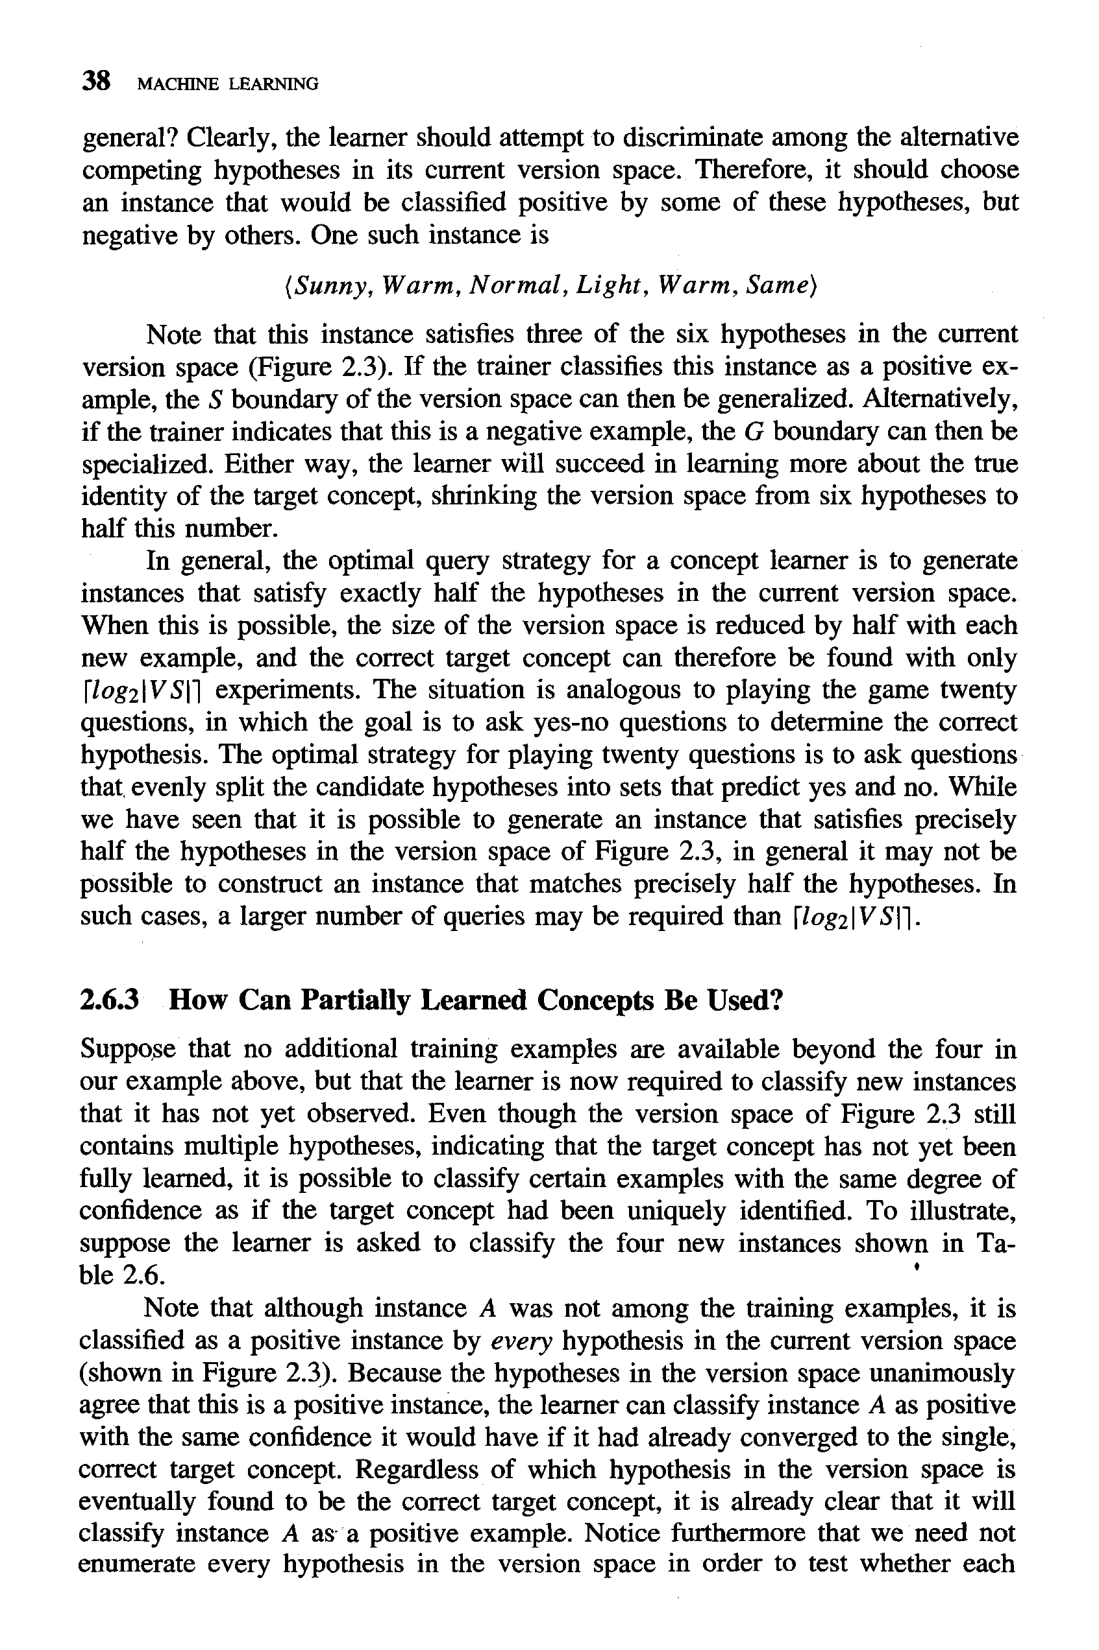
\includegraphics[width=0.9\linewidth]{figures/p50_b0.png}
\end{figure}

Tổng quan? Rõ ràng, người học nên cố gắng phân biệt giữa các giả thuyết cạnh tranh thay thế trong version space hiện tại của nó. Do đó, nên chọn một trường hợp được được phân loại là tích cực theo một số giả thuyết này nhưng lại là tiêu cực theo những giả thuyết khác. Một trường hợp như vậy là

\subsection{(Nắng, Ấm áp, Bình thường, Nhẹ nhàng, Ấm áp, Tương tự)}

Lưu ý rằng trường hợp này thỏa mãn ba trong số sáu giả thuyết trong hiện tại

Version space (Hình 2.3). Nếu người training classification trường hợp này là một ví dụ tích cực thì ranh giới S của version space khi đó có thể được khái quát hóa. Ngoài ra, nếu người training chỉ ra rằng đây là một ví dụ tiêu cực thì ranh giới G có thể là

Chuyên. Dù bằng cách nào, người học sẽ thành công trong việc tìm hiểu thêm về sự thật

Danh tính của khái niệm mục tiêu, thu hẹp version space từ sáu giả thuyết xuống còn một nửa con số này.

Nói chung, chiến lược truy vấn tối ưu cho người học khái niệm là tạo ra

Các trường hợp thỏa mãn chính xác một nửa giả thuyết trong version space hiện tại. Khi điều này có thể thực hiện được, kích thước của version space sẽ giảm đi một nửa với mỗi ví dụ mới và do đó chỉ có thể tìm thấy khái niệm mục tiêu chính xác với

Thí nghiệm rlog2JVS11. Tình huống tương tự như chơi trò chơi hai mươi

Câu hỏi, trong đó mục tiêu là đặt câu hỏi có-không để xác định giả thuyết đúng. Chiến lược tối ưu để chơi 20 câu hỏi là đặt những câu hỏi chia đều các giả thuyết của ứng viên thành các nhóm dự đoán có và không. Mặc dù chúng ta đã thấy rằng có thể tạo ra một individual thỏa mãn chính xác một nửa giả thuyết trong version space của Hình 2.3, nhưng nói chung không thể xây dựng một individual khớp chính xác với một nửa giả thuyết. Trong những trường hợp như vậy, có thể cần số lượng truy vấn lớn hơn rlog21VS(1.

\subsubsection{Có thể sử dụng các khái niệm đã học một phần như thế nào?}

Giả sử rằng không có ví dụ training bổ sung nào ngoài bốn ví dụ trong ví dụ trên của chúng ta, nhưng người học hiện được yêu cầu classification các trường hợp mới mà nó chưa quan sát được. Mặc dù version space của Hình 2.3 vẫn chứa nhiều giả thuyết, chỉ ra rằng khái niệm mục tiêu vẫn chưa được học đầy đủ, nhưng có thể classification một số ví dụ nhất định với cùng mức độ tin cậy như thể khái niệm mục tiêu đã được xác định duy nhất. Để minh họa, giả sử người học được yêu cầu classification bốn trường hợp mới được hiển thị trong Ta-

Ble 2.6.

% 9
Lưu ý rằng mặc dù trường hợp A không nằm trong số các ví dụ training, nhưng nó

Được được phân loại là một trường hợp tích cực theo mọi giả thuyết trong version space hiện tại (được hiển thị trong Hình 2.3). Bởi vì các giả thuyết trong version space nhất trí đồng ý rằng đây là một trường hợp tích cực, người học có thể classification trường hợp A là tích cực với cùng độ tin cậy nếu nó đã hội tụ về một trường hợp duy nhất,

Khái niệm mục tiêu chính xác. Bất kể giả thuyết nào trong version space cuối cùng được coi là khái niệm mục tiêu chính xác, thì rõ ràng là nó sẽ classification trường hợp A là một ví dụ tích cực. Ngoài ra, hãy lưu ý rằng chúng ta không cần liệt kê mọi giả thuyết trong version space để kiểm tra xem mỗi giả thuyết có

% --- page 51 ---
\begin{figure}[ht]
\centering
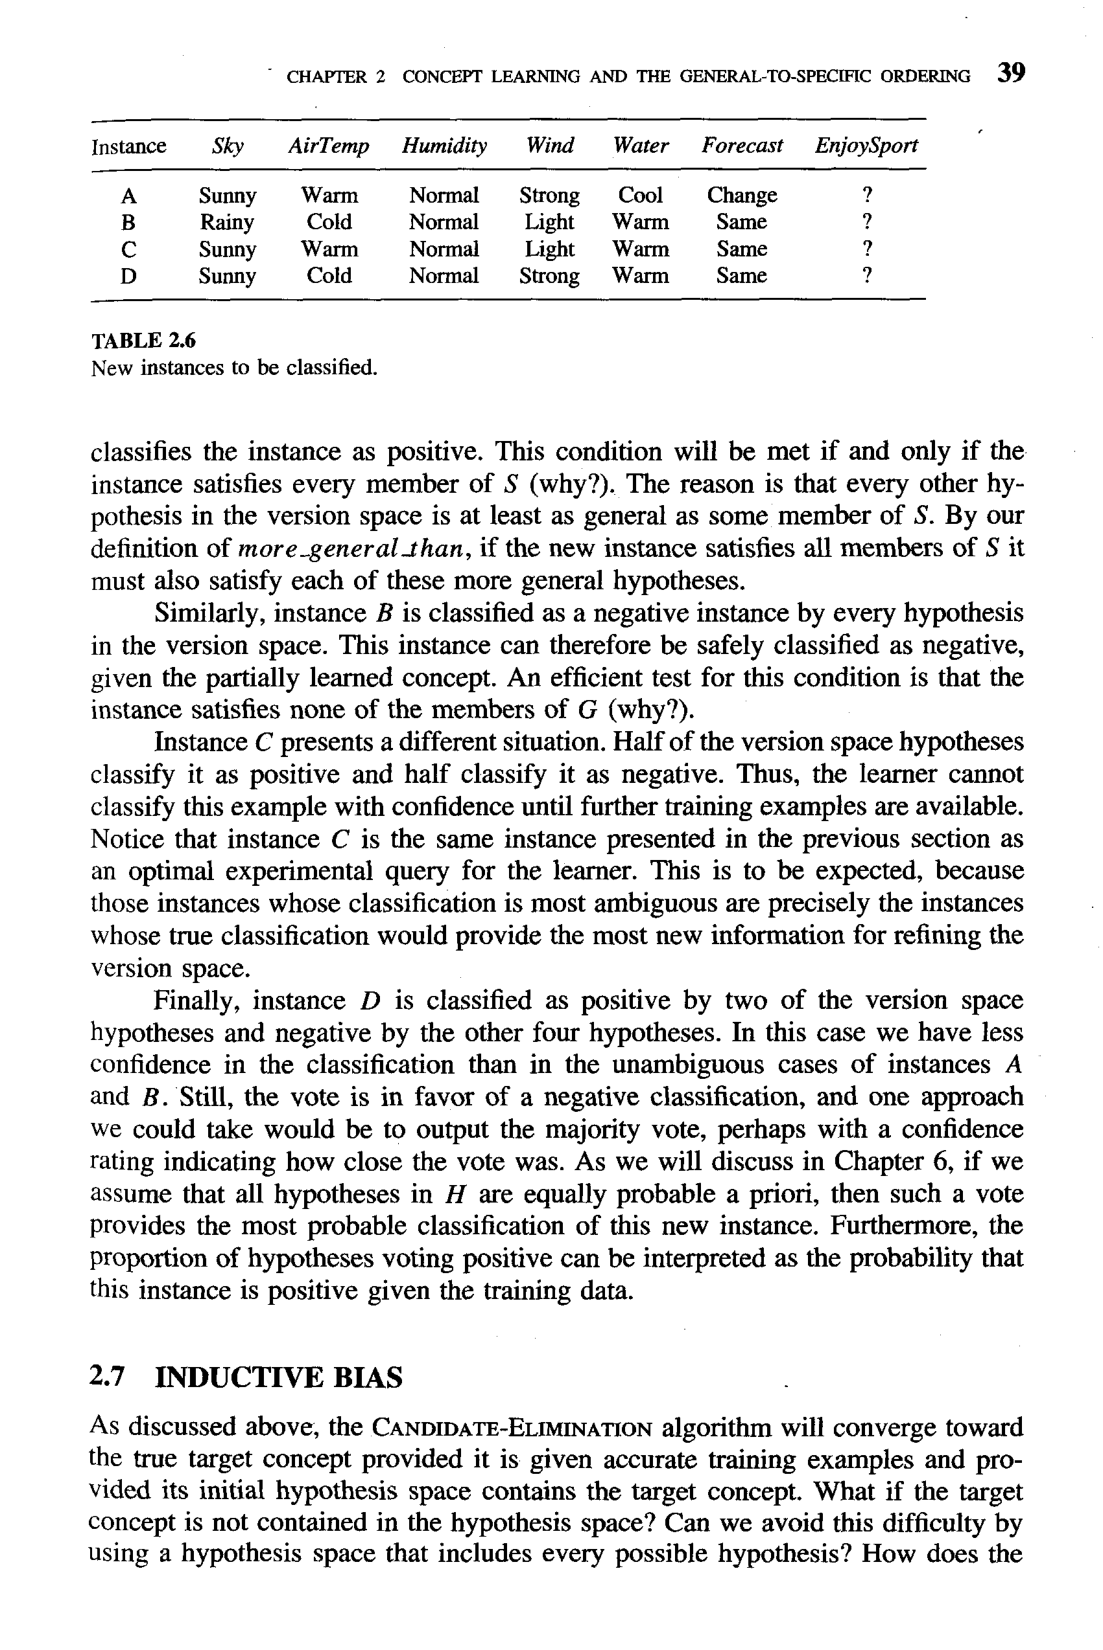
\includegraphics[width=0.9\linewidth]{figures/p51_b0.png}
\end{figure}

\subsection{CHAPTER 2 CONCEPT LEARNING AND THE GENERAL-TO-SPECIFIC ORDERING 39}

\subsection{Dự báo nước gió độ ẩm trên bầu trời AirTemp EnjoySport -}

Nắng ấm Bình thường Mạnh mẽ Thay đổi mát mẻ ?

B Mưa Lạnh Bình thường Ánh sáng Ấm áp Giống nhau ?

C Nắng Ấm Bình Thường Nắng Ấm Giống nhau ?

D Nắng Lạnh Bình thường Mạnh Ấm Tương tự ?

\noindent\textit{TABLE 2.6 Các trường hợp mới được phân loại.}

Classification trường hợp này là tích cực. Điều kiện này sẽ được đáp ứng khi và chỉ khi thể hiện thỏa mãn mọi thành viên của S (tại sao?). Lý do là mọi giả thuyết khác trong version space ít nhất cũng tổng quát như một thành viên nào đó của S. Theo định nghĩa của chúng ta về tổng quát hơn\textasciitilde{}han, nếu individual mới thỏa mãn tất cả các thành viên của S thì nó cũng phải thỏa mãn từng giả thuyết tổng quát hơn này.

Tương tự, trường hợp B được được phân loại là trường hợp phủ định theo mọi giả thuyết

Trong version space. Do đó, trường hợp này có thể được phân loại một cách an toàn là tiêu cực, dựa trên khái niệm đã học được một phần. Một phép kiểm tra hiệu quả cho điều kiện này là individual đó không thỏa mãn thành viên nào của G (tại sao?).

Trường hợp C trình bày một tình huống khác. Một nửa số giả thuyết version space

Classification nó là tích cực và một nửa classification nó là tiêu cực. Vì vậy, người học không thể tự tin classification mẫu này cho đến khi có thêm các mẫu training khác. Lưu ý rằng trường hợp C là trường hợp tương tự được trình bày trong phần trước như

Một truy vấn thử nghiệm tối ưu cho người học. Điều này được mong đợi bởi vì

Những trường hợp có classification mơ hồ nhất chính là những trường hợp có classification thực sự sẽ cung cấp thông tin mới nhất để tinh chỉnh version space.

Cuối cùng, phiên bản D được được phân loại là tích cực bởi hai trong số version space

Giả thuyết và phủ định bốn giả thuyết còn lại. Trong trường hợp này, chúng ta ít tin tưởng vào classification hơn so với các trường hợp rõ ràng của trường hợp A và B. Tuy nhiên, cuộc bỏ phiếu ủng hộ classification phủ định và một cách tiếp cận mà chúng ta có thể thực hiện là đưa ra đa số phiếu bầu, có lẽ với xếp hạng độ tin cậy cho thấy mức độ gần gũi của cuộc bỏ phiếu. Như chúng ta sẽ thảo luận trong Chương 6, nếu chúng ta giả định rằng tất cả các giả thuyết trong H đều có xác suất tiên nghiệm như nhau, thì việc bỏ phiếu như vậy sẽ mang lại classification có khả năng xảy ra cao nhất cho trường hợp mới này. Hơn nữa, tỷ lệ các giả thuyết bỏ phiếu tích cực có thể được hiểu là xác suất trường hợp này là tích cực dựa trên dữ liệu training.

\subsection{INDUCTIVE BIAS}

Như đã thảo luận ở trên, thuật toán CANDIDATE-ELIMINATION sẽ hội tụ về phía

Khái niệm mục tiêu thực sự với điều kiện nó được cung cấp các ví dụ training chính xác và hypothesis space ban đầu của nó có chứa khái niệm mục tiêu. Điều gì sẽ xảy ra nếu khái niệm mục tiêu không có trong hypothesis space? Liệu chúng ta có thể tránh được khó khăn này bằng cách sử dụng hypothesis space bao gồm mọi giả thuyết có thể xảy ra không? Làm thế nào

% --- page 52 ---
\begin{figure}[ht]
\centering
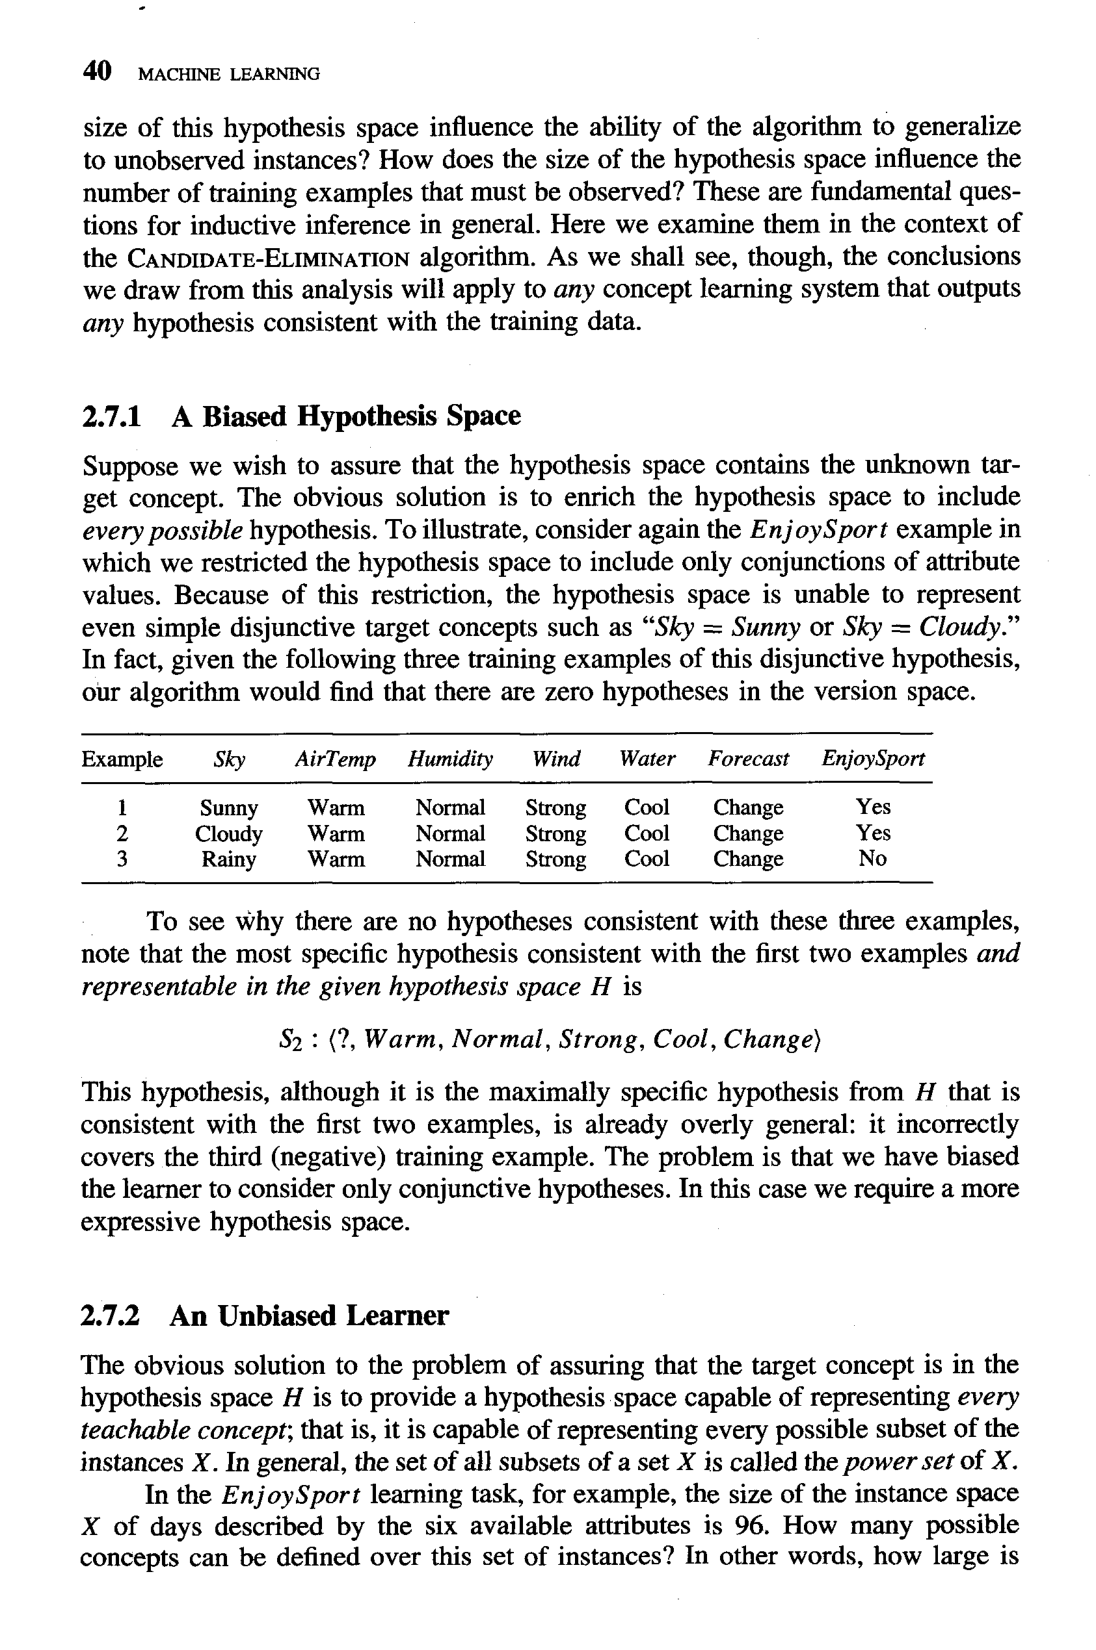
\includegraphics[width=0.9\linewidth]{figures/p52_b0.png}
\end{figure}

Kích thước của hypothesis space này có ảnh hưởng đến khả năng khái quát hóa thuật toán cho các trường hợp không quan sát được không? Kích thước của hypothesis space ảnh hưởng như thế nào đến số lượng mẫu training phải được quan sát? Đây là những câu hỏi cơ bản cho suy luận quy nạp nói chung. Ở đây chúng ta kiểm tra chúng trong bối cảnh thuật toán CANDIDATE-ELIMINATION. Tuy nhiên, như chúng ta sẽ thấy, các kết luận

Chúng ta rút ra từ phân tích này sẽ áp dụng cho bất kỳ hệ thống concept learning nào đưa ra bất kỳ giả thuyết nào phù hợp với dữ liệu training.

\subsubsection{Hypothesis Space bias}

Giả sử chúng ta muốn đảm bảo rằng hypothesis space chứa khái niệm mục tiêu chưa xác định. Giải pháp hiển nhiên là làm phong phú hypothesis space để bao gồm mọi giả thuyết có thể có. Để minh họa, hãy xem xét lại ví dụ EnjoySpor t trong đó chúng ta đã hạn chế hypothesis space chỉ bao gồm các liên kết của các giá trị thuộc tính. Do hạn chế này, hypothesis space không thể thể hiện ngay cả những khái niệm mục tiêu phân biệt đơn giản như "Bầu trời = Nắng hoặc Bầu trời = Mây." Trên thực tế, với ba ví dụ training sau đây về giả thuyết phân tách này, thuật toán của chúng ta sẽ thấy rằng không có giả thuyết nào trong version space.

Ví dụ Bầu trời AirTemp Độ ẩm Gió Nước Dự báo EnjoySport

\section{Nắng Ấm Bình thường Mạnh Mát Thay đổi Có}

\section{Mây Ấm Bình thường Mạnh Mát Thay đổi Có}

\section{Mưa Ấm Bình thường Mạnh Mát Thay đổi Không}

Để biết tại sao không có giả thuyết nào phù hợp với ba ví dụ này,

Lưu ý rằng giả thuyết cụ thể nhất phù hợp với hai ví dụ đầu tiên và

\subsection{Có thể biểu diễn trong hypothesis space H đã cho là}

S2 : (?, Ấm áp, Bình thường, Mạnh mẽ, Mát mẻ, Thay đổi)

Giả thuyết này, mặc dù giả thuyết cụ thể tối đa từ H phù hợp với hai ví dụ đầu tiên, nhưng đã quá chung chung: nó bao hàm không chính xác ví dụ training thứ ba (tiêu cực). Vấn đề là chúng ta đã bias người học chỉ xem xét các giả thuyết liên kết. Trong trường hợp này, chúng ta yêu cầu hypothesis space có tính biểu cảm cao hơn.

\subsubsection{Người học không bias}

Giải pháp rõ ràng cho vấn đề đảm bảo rằng khái niệm đích có trong hypothesis space H là cung cấp hypothesis space có khả năng thể hiện mọi khái niệm có thể dạy được; nghĩa là nó có khả năng biểu diễn mọi tập con có thể có của

Trường hợp X. Nói chung, tập hợp tất cả các tập con của tập X được gọi là tập lũy thừa của X.

Ví dụ: trong nhiệm vụ học tập EnjoySport, kích thước của version space

X số ngày được mô tả bởi sáu thuộc tính có sẵn là 96. Có bao nhiêu khái niệm có thể được xác định trên tập hợp các trường hợp này? Nói cách khác, nó lớn đến mức nào

% --- page 53 ---
\begin{figure}[ht]
\centering
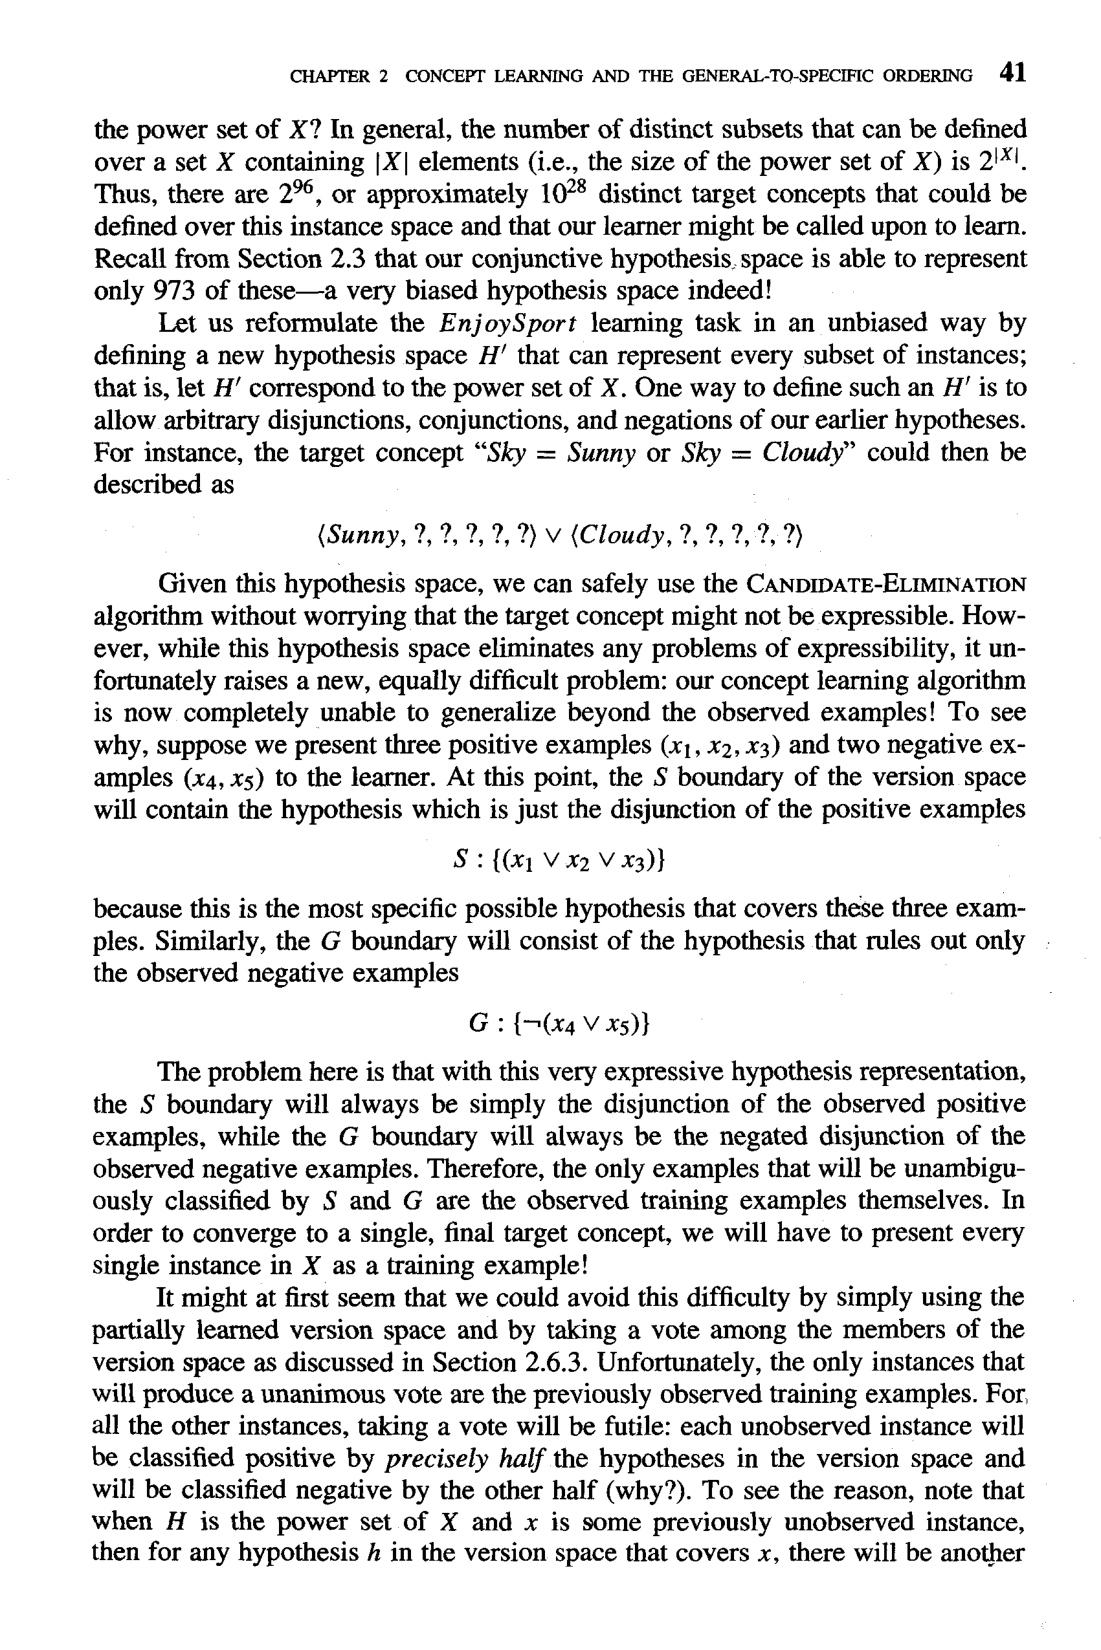
\includegraphics[width=0.9\linewidth]{figures/p53_b0.png}
\end{figure}

Tập lũy thừa của X? Nói chung, số lượng các tập con riêng biệt có thể được xác định trên một tập X chứa các phần tử 1x1 (tức là kích thước của tập lũy thừa của X) là 21'1. Vì vậy, có 296 hoặc gần đúng khái niệm mục tiêu riêng biệt có thể được

Được xác định trên không gian individual này và người học của chúng ta có thể được yêu cầu học hỏi. Hãy nhớ lại từ Phần 2.3 rằng hypothesis space liên hợp của chúng ta chỉ có thể biểu diễn 973 trong số này - một hypothesis space thực sự rất sai lệch!

Chúng ta hãy xây dựng lại nhiệm vụ học tập Enjoysport một cách khách quan bằng cách

Xác định hypothesis space H' mới có thể đại diện cho mọi tập hợp con của các phiên bản; nghĩa là, giả sử H' tương ứng với tập lũy thừa của X. Một cách để định nghĩa một H' như vậy là cho phép phân tách, kết hợp và phủ định tùy ý các giả thuyết trước đó của chúng ta. Ví dụ: khái niệm mục tiêu "Bầu trời = Nắng hoặc Bầu trời = Mây" khi đó có thể được mô tả là

(Nắng, ?, ?, ?, ?, ?) v (Mây, ?, ?, ?, ?, ?)

Với hypothesis space này, chúng ta có thể sử dụng CANDIDATE-ELIMINATION một cách an toàn

Thuật toán mà không phải lo lắng rằng khái niệm mục tiêu có thể không diễn đạt được. Tuy nhiên, trong khi hypothesis space này loại bỏ mọi vấn đề về khả năng biểu đạt, thật không may, nó lại nảy sinh một vấn đề mới, khó khăn không kém: thuật toán concept learning của chúng ta hiện hoàn toàn không thể khái quát hóa ngoài các ví dụ được quan sát! Để biết lý do tại sao, giả sử chúng ta trình bày ba ví dụ tích cực (xl, $x_{2}$, $x_{3}$) và hai ví dụ tiêu cực

Dồi dào ($x_{4}$, $x_{5}$) cho người học. Tại thời điểm này, ranh giới S của version space sẽ chứa giả thuyết chỉ là sự phân tách của các ví dụ tích cực

Bởi vì đây là giả thuyết cụ thể nhất có thể bao hàm ba ví dụ này. Tương tự, ranh giới G sẽ bao gồm giả thuyết chỉ loại trừ các ví dụ tiêu cực được quan sát.

Vấn đề ở đây là với cách trình bày giả thuyết rất biểu cảm này,

Ranh giới S sẽ luôn đơn giản là sự phân tách của các ví dụ tích cực được quan sát, trong khi ranh giới G sẽ luôn là sự phân tách phủ định của các ví dụ tiêu cực được quan sát. Do đó, các ví dụ duy nhất sẽ được phân loại rõ ràng bởi S và G chính là các ví dụ training được quan sát. Để hội tụ đến một khái niệm mục tiêu cuối cùng, duy nhất, chúng ta sẽ phải trình bày mọi phiên bản trong X làm ví dụ training!

Thoạt đầu có vẻ như chúng ta có thể tránh được khó khăn này bằng cách sử dụng

Đã học được một phần version space và bằng cách bỏ phiếu giữa các thành viên của version space như được thảo luận trong Phần 2.6.3. Thật không may, những trường hợp duy nhất tạo ra sự bỏ phiếu nhất trí là những ví dụ training đã được quan sát trước đó. Vì, tất cả các trường hợp khác, việc bỏ phiếu sẽ vô ích: mỗi trường hợp không được quan sát sẽ được được phân loại là tích cực theo đúng một nửa số giả thuyết trong version space và sẽ được được phân loại là tiêu cực bởi nửa còn lại (tại sao?). Để hiểu lý do, hãy lưu ý rằng khi H là tập lũy thừa của X và x là một trường hợp nào đó chưa được quan sát trước đó, thì với bất kỳ giả thuyết h nào trong version space bao phủ x, sẽ có anoQer

% --- page 54 ---
\begin{figure}[ht]
\centering
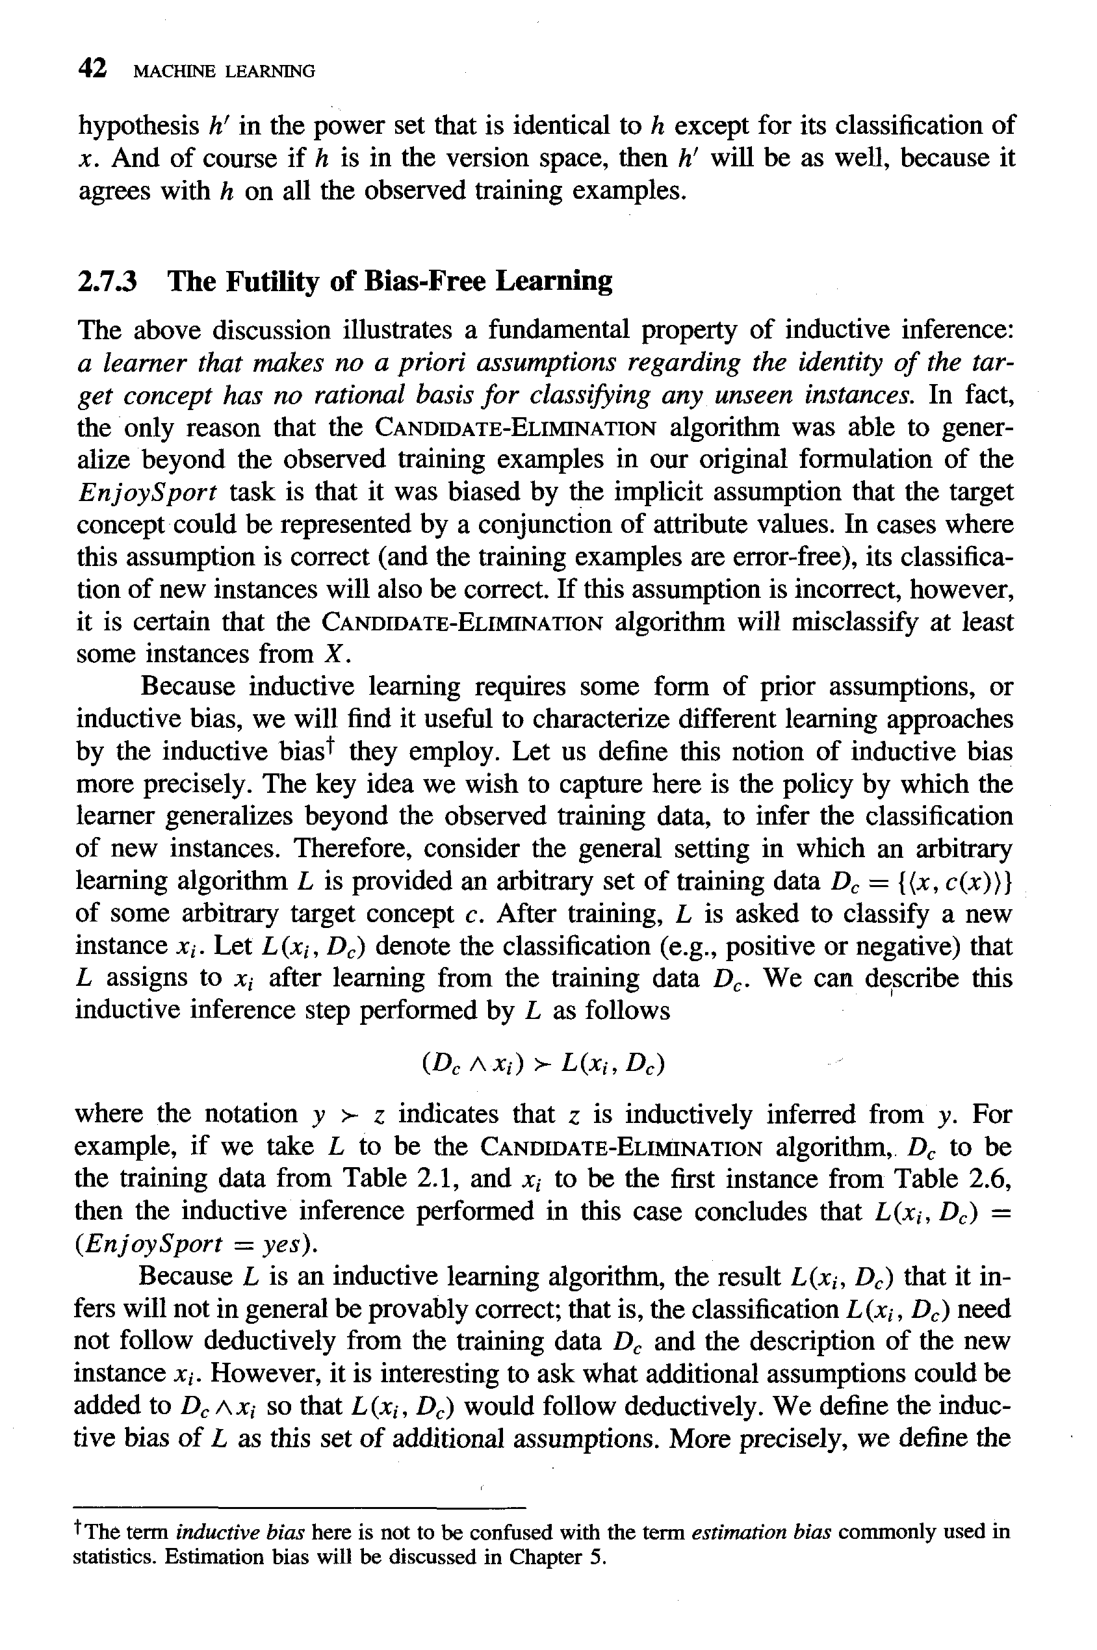
\includegraphics[width=0.9\linewidth]{figures/p54_b0.png}
\end{figure}

Giả thuyết h' trong tập lũy thừa giống với h ngoại trừ classification của nó là x. Và tất nhiên nếu h nằm trong version space thì h' cũng sẽ như vậy, vì nó phù hợp với h trên tất cả các ví dụ training được quan sát.

\subsubsection{Sự vô ích của việc học không cần Bias}

Cuộc thảo luận ở trên minh họa một đặc tính cơ bản của suy luận quy nạp: một người học không đưa ra các giả định tiên nghiệm về nhận dạng của khái niệm mục tiêu sẽ không có cơ sở hợp lý để classification bất kỳ trường hợp không nhìn thấy nào. Trên thực tế, lý do duy nhất khiến thuật toán CANDIDATE-ELIMINATION có thể tạo ra

Ngoài các ví dụ training được quan sát trong công thức ban đầu của chúng ta về nhiệm vụ EnjoySport là nó bị sai lệch bởi giả định ngầm rằng mục tiêu

Khái niệm có thể được biểu diễn bằng sự kết hợp của các giá trị thuộc tính. Trong trường hợp giả định này đúng (và các ví dụ training không có lỗi), classification của các phiên bản mới cũng sẽ đúng. Tuy nhiên, nếu giả định này không chính xác thì chắc chắn rằng thuật toán CANDIDATE-ELIMINATION sẽ classification ít nhất

Một số trường hợp từ X.

Bởi vì inductive learning yêu cầu một số dạng giả định trước đó, hoặc

Inductive bias, chúng ta sẽ thấy hữu ích khi mô tả các phương pháp học tập khác nhau bằng thành kiến ​​quy nạp mà chúng sử dụng. Chúng ta hãy định nghĩa khái niệm inductive bias này một cách chính xác hơn. Ý tưởng chính mà chúng ta muốn nắm bắt ở đây là chính sách mà người học sử dụng để khái quát hóa ngoài dữ liệu training được quan sát, để suy ra classification của các phiên bản mới. Do đó, hãy xem xét cài đặt chung trong đó thuật toán học tùy ý L được cung cấp một dataset training tùy ý D, = \{(x, c(x))\} của một số khái niệm mục tiêu tùy ý c. Sau khi training, L được yêu cầu classification một thể hiện mới xi. Đặt L(xi, D,) biểu thị classification (ví dụ: dương hoặc âm) mà L gán cho xi sau khi học từ dữ liệu training D,. Chúng ta có thể mô tả bước suy luận quy nạp được thực hiện bởi L như sau

Trong đó ký hiệu y + z chỉ ra rằng z được suy ra theo phương pháp quy nạp từ y. Ví dụ: nếu chúng ta lấy L là thuật toán CANDIDATE-ELIMINATION, D là

Dữ liệu training từ Bảng 2.1 và xi là trường hợp đầu tiên từ Bảng 2.6, thì suy luận quy nạp được thực hiện trong trường hợp này kết luận rằng L(xi, D,) =

\[(EnjoySport = yes).\]

Vì L là thuật toán inductive learning nên kết quả L(xi, D,) mà nó đưa ra-

Các ý kiến ​​nói chung sẽ không được chứng minh là chính xác; nghĩa là, classification L(xi, D,) không cần phải suy diễn từ dữ liệu training D và mô tả của phiên bản mới xi. Tuy nhiên, thật thú vị khi hỏi những giả định bổ sung nào có thể được thêm vào D, r\textbackslash{}xi để L(xi, D,) tuân theo suy diễn. Chúng ta xác định inductive bias của L là tập hợp các giả định bổ sung này. Chính xác hơn, chúng ta định nghĩa

T \textasciitilde{} h e thuật ngữ inductive bias ở đây không được nhầm lẫn với thuật ngữ ước tính bias thường được sử dụng trong

Số liệu thống kê. Ước tính bias sẽ được thảo luận trong Chương 5.

% --- page 55 ---
\begin{figure}[ht]
\centering
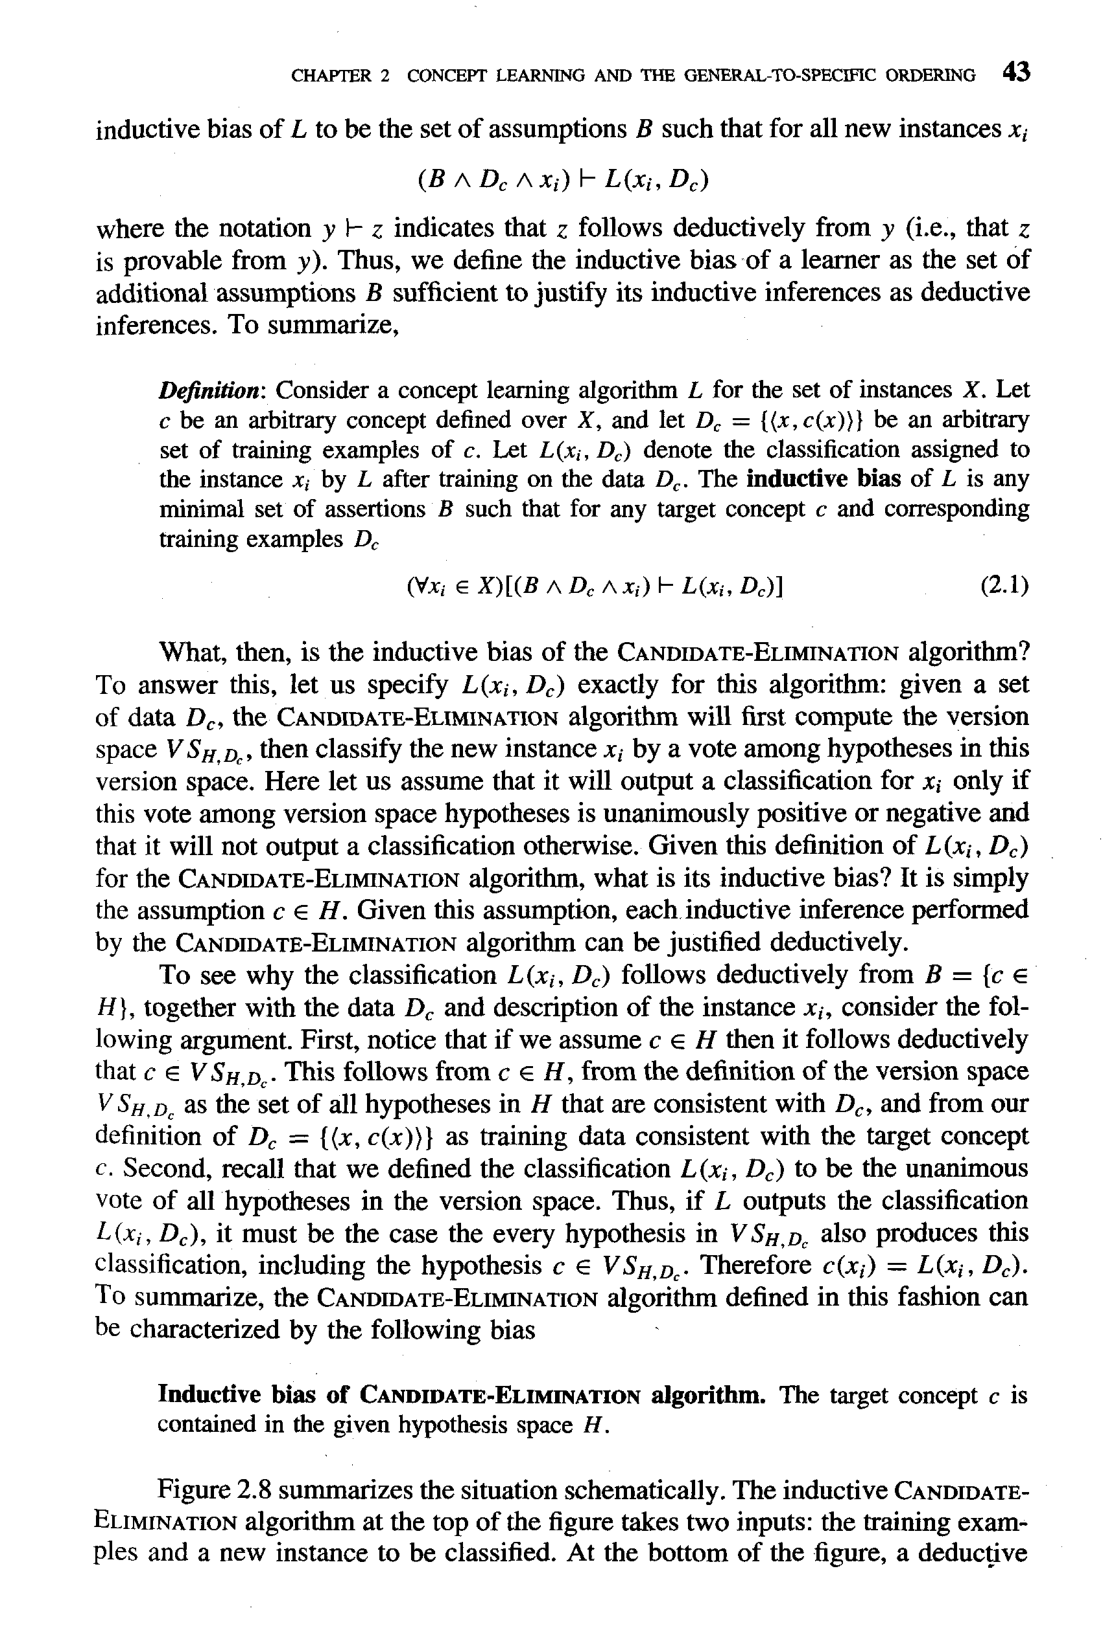
\includegraphics[width=0.9\linewidth]{figures/p55_b0.png}
\end{figure}

\subsection{CHAFI\%R 2 CONCEPT LEARNING AND THE GENERAL-TO-SPECIFIC ORDERING 43}

Inductive bias của L là tập hợp các giả định B sao cho với mọi trường hợp mới xi

( B A D, A xi) F L(xi, D,)

Trong đó ký hiệu y t z chỉ ra rằng z suy diễn từ y (tức là z có thể chứng minh được từ y). Do đó, chúng ta định nghĩa inductive bias của người học là tập hợp các giả định B bổ sung đủ để chứng minh các suy luận quy nạp của nó là các suy luận suy diễn. Tóm lại,

Định nghĩa: Xét thuật toán concept learning L cho tập hợp các phiên bản X. Giả sử

C là một khái niệm tùy ý được xác định trên X và đặt D, = ( ( x , c(x))\} là một khái niệm tùy ý

Tập các ví dụ training của c. Đặt L(xi, D,) biểu thị classification được gán cho

Thể hiện xi của L sau khi training trên dữ liệu D,. Inductive bias của L là tập tối thiểu bất kỳ của các xác nhận B sao cho đối với mọi khái niệm mục tiêu c và các ví dụ training tương ứng Dc

(Vxi E X)[(B A Dc A xi) k L(xi, D,)] (2.1)

Vậy inductive bias của thuật toán CANDIDATE-ELIMINATION là gì?

Để trả lời câu hỏi này, chúng ta hãy chỉ định chính xác L(xi, D,) cho thuật toán này: với một dataset D, thuật toán CANDIDATE-ELIMINATION trước tiên sẽ tính toán phiên bản

Không gian VSH,D, sau đó classification phiên bản mới xi bằng cách bỏ phiếu giữa các giả thuyết trong version space này. Ở đây chúng ta hãy giả sử rằng nó sẽ tạo ra classification cho xi chỉ khi cuộc bỏ phiếu này trong số các giả thuyết version space là tích cực hoặc tiêu cực và nếu không thì nó sẽ không tạo ra classification. Với định nghĩa L(xi, D,) này cho thuật toán CANDIDATE-ELIMINATION, inductive bias của nó là gì? Nó đơn giản là

Giả định c E H. Với giả định này, mỗi suy luận quy nạp được thực hiện bởi thuật toán CANDIDATE-ELIMINATION có thể được chứng minh bằng phương pháp suy diễn.

Để biết tại sao classification L(xi, D,) suy diễn theo cách suy diễn từ B = \{c E

H), cùng với dữ liệu D và mô tả của thể hiện xi, hãy xem xét các công thức sau:

Hạ thấp lý lẽ. Đầu tiên, lưu ý rằng nếu chúng ta giả sử c E H thì suy diễn ra c E VSH,Dc. Điều này tuân theo c E H, từ định nghĩa của version space

VSH,D, là tập hợp tất cả các giả thuyết trong H phù hợp với D, và từ

Định nghĩa D, = \{(x, c(x))\} là dữ liệu training phù hợp với khái niệm đích c. Thứ hai, hãy nhớ lại rằng chúng ta đã định nghĩa classification L(xi, D,) là biểu quyết nhất trí của tất cả các giả thuyết trong version space. Do đó, nếu L tạo ra classification L(x,, D,), thì chắc chắn mọi giả thuyết trong V S H , \textasciitilde{} , cũng tạo ra kết quả này

Classification, trong đó có giả thuyết c E VSHYDc. Do đó c(xi) = L(xi, D,).

Tóm lại, thuật toán CANDIDATE-ELIMINATION được xác định theo cách này có thể

\subsection{Được feature bởi bias sau đây}

Inductive bias của thuật toán CANDIDATE-ELIMINATION. Khái niệm mục tiêu c là

Chứa trong hypothesis space H đã cho.

\noindent\textit{Hình 2.8 tóm tắt tình hình một cách sơ đồ. CANDIDATE- cảm ứng}

Thuật toán ELIMINATION ở đầu hình có hai đầu vào: bài kiểm tra training-

Ples và một individual mới cần được phân loại. Ở dưới cùng của hình là một suy luận

% --- page 56 ---
\begin{figure}[ht]
\centering
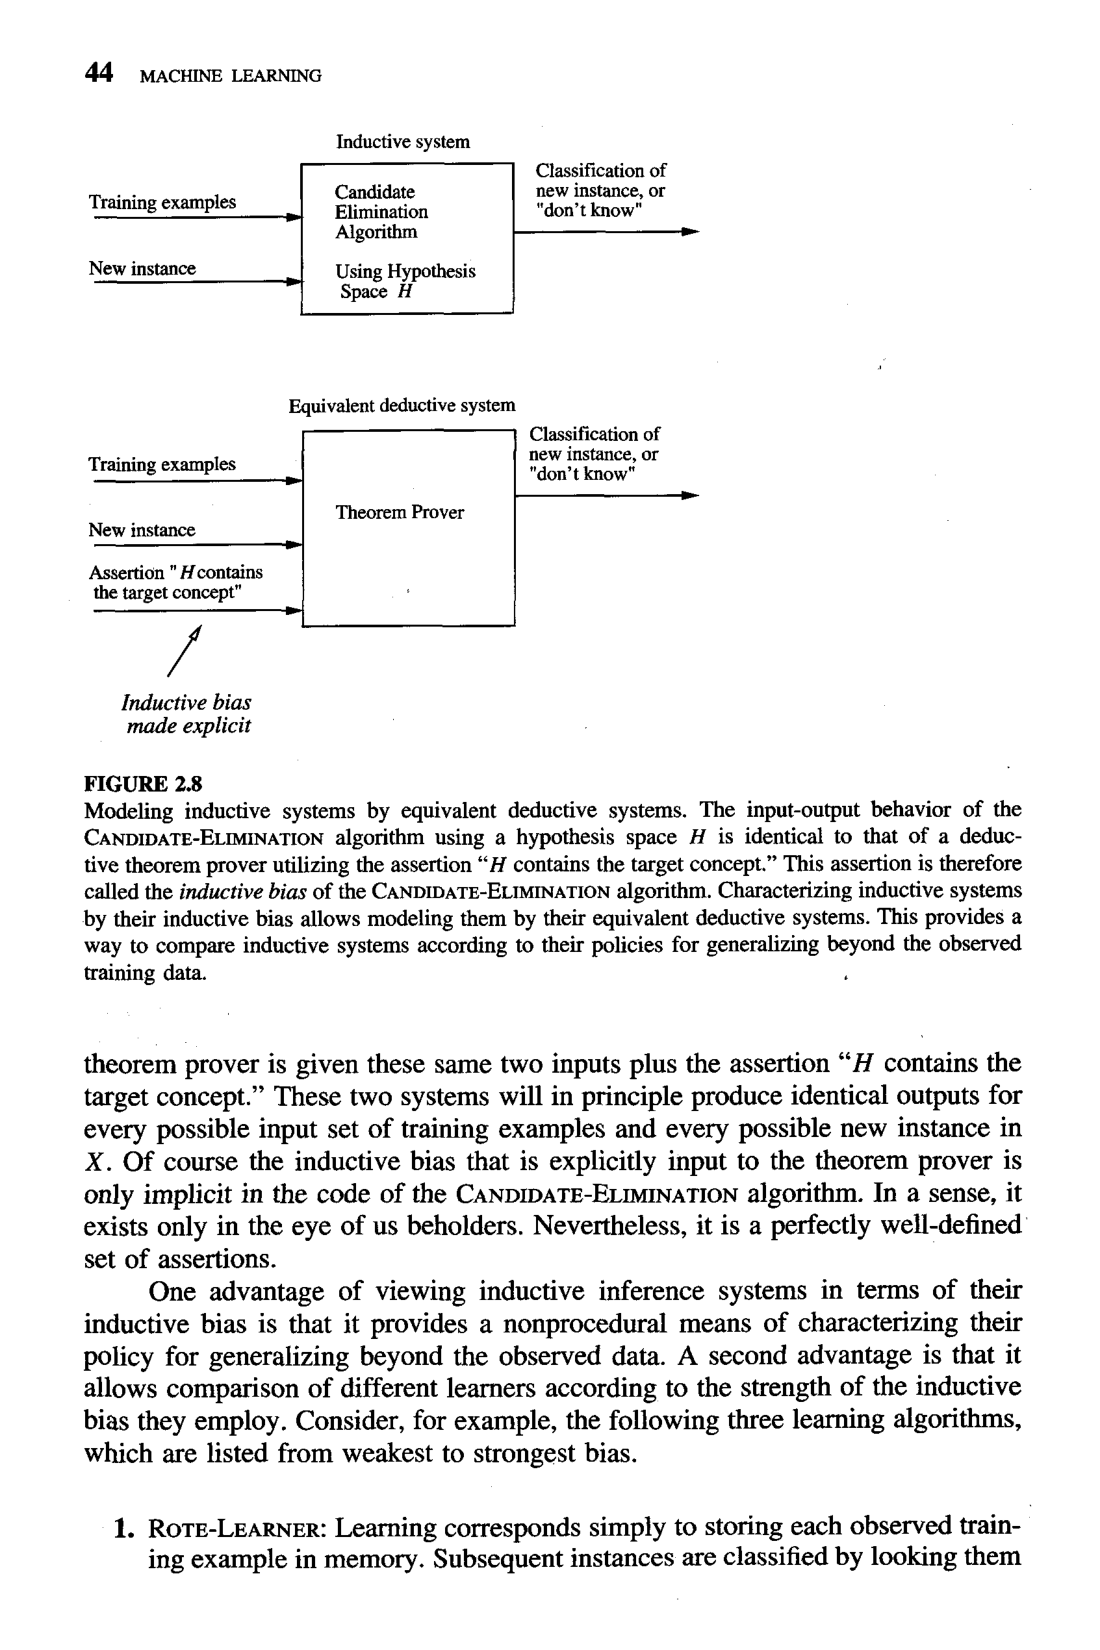
\includegraphics[width=0.9\linewidth]{figures/p56_b0.png}
\end{figure}

\section{MACHINE LEARNING}

Hệ thống cảm ứng

Classification của

Thí sinh mới, hoặc Ví dụ training Loại bỏ "không biết"

Trường hợp mới sử dụng giả thuyết

Space H

Equivalent deductive system

Tôi tôi Classification của

\subsection{Training examples I}

new instance, or "don't know"

Chứng minh định lý

Khẳng định “H chứa

Khái niệm mục tiêu”

-D

P

Inductive bias

Làm rõ ràng

\noindent\textit{FIGURE 2.8 Model hóa hệ thống quy nạp bằng hệ thống suy diễn tương đương. Hành vi đầu vào-đầu ra của thuật toán CANDIDATE-ELIMINATION sử dụng hypothesis space H giống hệt với hành vi của thuật toán suy luận.}

Tive theorem prover utilizing the assertion "H contains the target concept." Do đó, xác nhận này được gọi là inductive bias của thuật toán CANDIDATE-ELIMINATION. Feature của hệ thống cảm ứng

by their inductive bias allows modeling them by their equivalent deductive systems. This provides a way to compare inductive systems according to their policies for generalizing beyond the observed training data.

theorem prover is given these same two inputs plus the assertion "H contains the target concept." These two systems will in principle produce identical outputs for every possible input set of training examples and every possible new instance in X. Of course the inductive bias that is explicitly input to the theorem prover is only implicit in the code of the CANDIDATE-ELIMINATION algorithm. In a sense, it

exists only in the eye of us beholders. Nevertheless, it is a perfectly well-defined

Tập hợp các khẳng định.

Một lợi thế của việc xem xét các hệ thống suy luận quy nạp về mặt

inductive bias is that it provides a nonprocedural means of characterizing their

Chính sách khái quát hóa ngoài dữ liệu được quan sát. Ưu điểm thứ hai là nó cho phép so sánh những người học khác nhau tùy theo sức mạnh của inductive bias mà họ sử dụng. Ví dụ: hãy xem xét ba thuật toán học sau đây, được liệt kê từ bias yếu nhất đến mạnh nhất.

1. ROTE-LEARNER: Việc học đơn giản tương ứng với việc lưu trữ từng đoàn tàu được quan sát-

Ví dụ trong bộ nhớ. Subsequent instances are classified by looking them

% --- page 57 ---
\begin{figure}[ht]
\centering
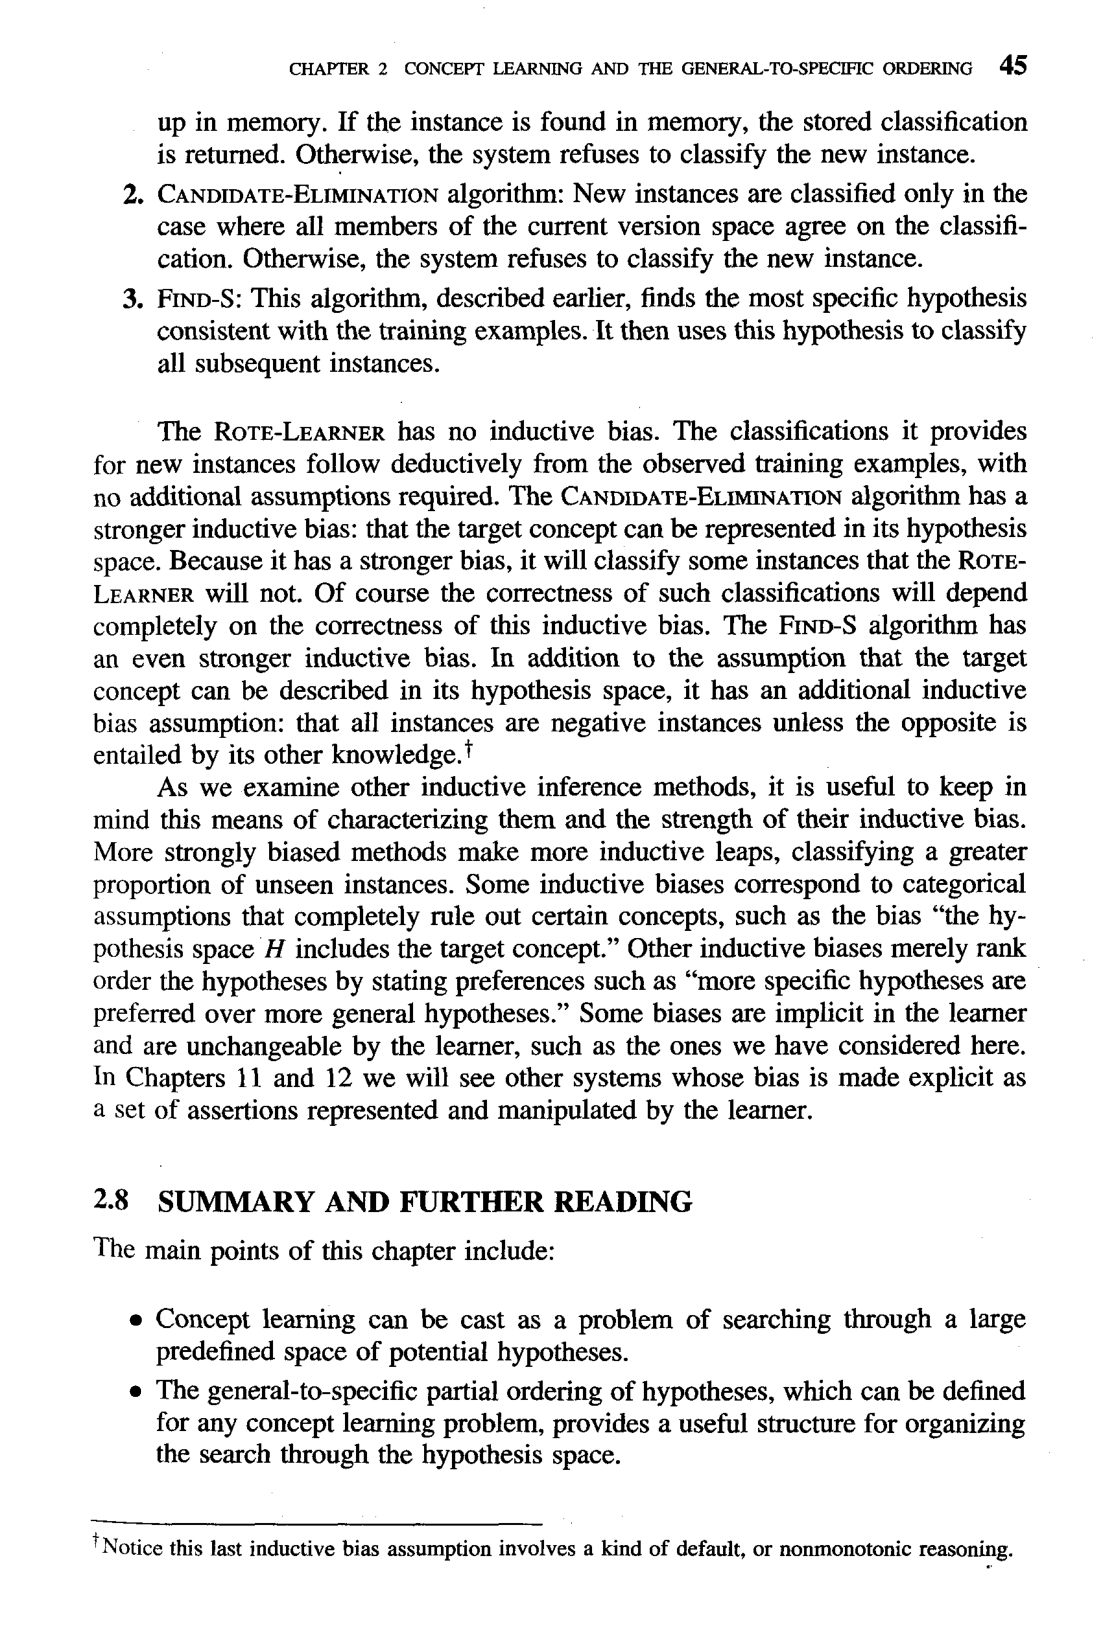
\includegraphics[width=0.9\linewidth]{figures/p57_b0.png}
\end{figure}

CHAPTER 2 CONCEPT. LEARNING AND THE GENERAL-TO-SPECIFIC ORDERING 45

Lên trong trí nhớ. If the instance is found in memory, the stored classification is returned. Otherwise, the system refuses to classify the new instance.

2. Thuật toán CANDIDATE-ELIMINATION: Các phiên bản mới chỉ được phân loại trong

Trường hợp tất cả các thành viên của version space hiện tại đồng ý về classification. Nếu không, hệ thống sẽ từ chối classification phiên bản mới.

3. FIND-S: Thuật toán này, được mô tả trước đó, tìm ra giả thuyết cụ thể nhất

Phù hợp với các ví dụ training. Sau đó nó sử dụng giả thuyết này để classification tất cả các trường hợp tiếp theo.

The ROTE-LEARNER has no inductive bias. The classifications it provides

Đối với các trường hợp mới, hãy làm theo cách suy diễn từ các ví dụ training được quan sát mà không cần thêm giả định nào. Thuật toán CANDIDATE-ELIMINATION có

Inductive bias mạnh hơn: khái niệm mục tiêu có thể được thể hiện trong hypothesis space của nó. Bởi vì nó có bias mạnh hơn nên nó sẽ classification một số trường hợp mà ROTELEARNER sẽ không classification. Tất nhiên tính đúng đắn của việc classification như vậy sẽ phụ thuộc vào

Hoàn toàn về tính đúng đắn của inductive bias này. Thuật toán FIND-S có inductive bias thậm chí còn mạnh hơn. Ngoài giả định rằng khái niệm mục tiêu có thể được mô tả trong hypothesis space của nó, nó còn có một giả định inductive bias bổ sung: rằng tất cả các trường hợp đều là trường hợp phủ định trừ khi điều ngược lại được kéo theo bởi các kiến ​​thức khác của nó.t

Khi chúng ta xem xét các phương pháp suy luận quy nạp khác, sẽ rất hữu ích khi giữ nguyên

Hãy nhớ phương tiện này để mô tả đặc điểm của chúng và sức mạnh inductive bias của chúng. Các phương pháp bias mạnh hơn tạo ra nhiều bước nhảy quy nạp hơn, classification tỷ lệ lớn hơn các trường hợp chưa nhìn thấy. Một số thành kiến ​​quy nạp tương ứng với thành kiến ​​classification

Giả định loại trừ hoàn toàn các khái niệm nhất định, chẳng hạn như bias "hy-

Không gian giả thuyết H bao gồm khái niệm mục tiêu." Các thành kiến ​​quy nạp khác chỉ đơn thuần xếp thứ tự các giả thuyết bằng cách nêu các ưu tiên chẳng hạn như "các giả thuyết cụ thể hơn được ưa thích hơn các giả thuyết tổng quát hơn." Một số thành kiến ​​tiềm ẩn trong người học và không thể thay đổi bởi người học, chẳng hạn như những thành kiến ​​mà chúng ta đã xem xét ở đây. Trong Chương 11 và 12, chúng ta sẽ thấy các hệ thống khác mà bias được trình bày rõ ràng như một tập hợp các xác nhận được đại diện và thao tác bởi người học.

\subsection{SUMMARY AND FURTHER READING}

Các điểm chính của chương này bao gồm:

Concept learning có thể được coi là một bài toán tìm kiếm trong một không gian rộng lớn được xác định trước của các giả thuyết tiềm năng. Thứ tự từng phần của các giả thuyết từ tổng quát đến cụ thể, có thể được xác định cho bất kỳ bài toán concept learning nào, cung cấp một cấu trúc hữu ích để tổ chức tìm kiếm thông qua hypothesis space.

+Lưu ý rằng giả định inductive bias cuối cùng này liên quan đến một loại lý luận mặc định hoặc không đơn điệu.

% --- page 58 ---
\begin{figure}[ht]
\centering
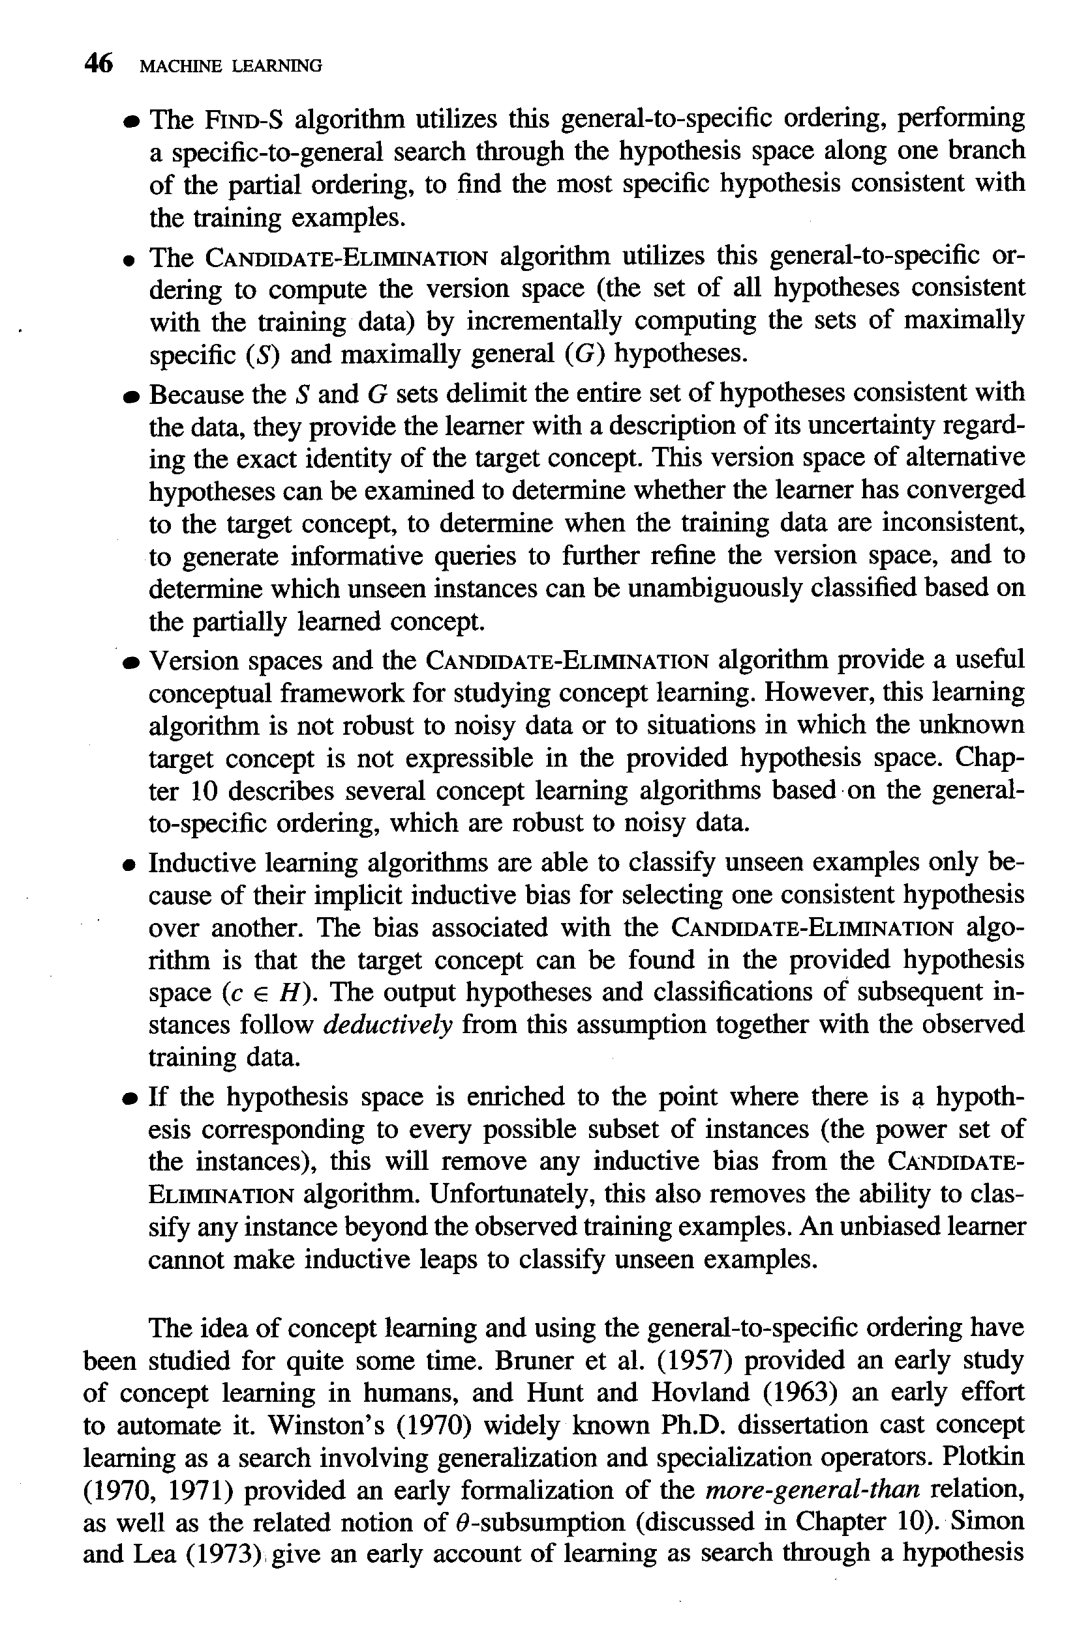
\includegraphics[width=0.9\linewidth]{figures/p58_b0.png}
\end{figure}

Thuật toán FINDS sử dụng thứ tự từ tổng quát đến cụ thể này, thực hiện tìm kiếm từ cụ thể đến tổng quát thông qua hypothesis space dọc theo một nhánh của thứ tự từng phần, để tìm ra giả thuyết cụ thể nhất phù hợp với các ví dụ training. Thuật toán CANDIDATE-ELIMINATION sử dụng thuật toán từ tổng quát đến cụ thể hoặc-

Để tính toán version space (tập hợp tất cả các giả thuyết phù hợp với dữ liệu training) bằng cách tính toán tăng dần các tập hợp giả thuyết cụ thể tối đa (S) và giả thuyết tổng quát tối đa (G).

Bởi vì các bộ S và G phân định toàn bộ tập hợp các giả thuyết nhất quán với dữ liệu nên chúng cung cấp cho người học bản mô tả về mức độ không chắc chắn của nó liên quan đến nhận dạng chính xác của khái niệm mục tiêu. Version space trong số các giả thuyết thay thế này có thể được kiểm tra để xác định xem người học có hội tụ đến khái niệm đích hay không, để xác định khi nào dữ liệu training không nhất quán, để tạo ra các truy vấn thông tin nhằm tinh chỉnh thêm version space và để xác định những trường hợp chưa nhìn thấy nào có thể được phân loại rõ ràng dựa trên khái niệm đã học một phần. Thuật toán Version spaces và CANDIDATE-ELIMINATION cung cấp một giải pháp hữu ích

Khung khái niệm để nghiên cứu concept learning. Tuy nhiên, thuật toán học này không mạnh đối với dữ liệu nhiễu hoặc đối với các tình huống trong đó khái niệm mục tiêu chưa xác định không thể diễn đạt được trong hypothesis space được cung cấp. Chương 10 mô tả một số thuật toán concept learning dựa trên thứ tự tổng quát đến cụ thể, phù hợp với dữ liệu nhiễu.

\section{Thuật toán Inductive learning chỉ có thể classification các mẫu không nhìn thấy được-}

Nguyên nhân dẫn đến inductive bias tiềm ẩn của họ trong việc lựa chọn giả thuyết nhất quán này thay vì giả thuyết khác. Bias được liên kết với thuật toán CANDIDATE-ELIMINATION

Điều đáng chú ý là khái niệm mục tiêu có thể được tìm thấy trong hypothesis space (c E H) được cung cấp. Các giả thuyết đầu ra và classification của các trường hợp tiếp theo được suy diễn từ giả định này cùng với dữ liệu training được quan sát. Nếu hypothesis space được làm phong phú đến mức có giả thuyết tương ứng với mọi tập hợp con có thể có của các trường hợp (tập lũy thừa của các trường hợp), điều này sẽ loại bỏ mọi inductive bias khỏi thuật toán CANDIDATEELIMINATION. Thật không may, điều này cũng loại bỏ khả năng classification

Xác định bất kỳ trường hợp nào ngoài các ví dụ training được quan sát. Một người học không bias không thể thực hiện những bước nhảy vọt quy nạp để classification các ví dụ không nhìn thấy được.

Ý tưởng về concept learning và việc sử dụng thứ tự từ tổng quát đến cụ thể đã

Đã được nghiên cứu khá lâu. Bruner và cộng sự. (1957) đã cung cấp một nghiên cứu ban đầu về concept learning ở người, còn Hunt và Hovland (1963) đã nỗ lực ban đầu để tự động hóa nó. Tiến sĩ được biết đến rộng rãi của Winston (1970). Luận án coi concept learning là một tìm kiếm liên quan đến các toán tử tổng quát hóa và chuyên môn hóa. Plotkin (1970, 1971) đã sớm đưa ra cách hình thức hóa quan hệ tổng quát hơn, cũng như khái niệm liên quan về giả định 8 (được thảo luận trong Chương 10). Simon và Lea (1973) đưa ra quan điểm ban đầu về việc học là tìm kiếm thông qua một giả thuyết

% --- page 59 ---
\begin{figure}[ht]
\centering
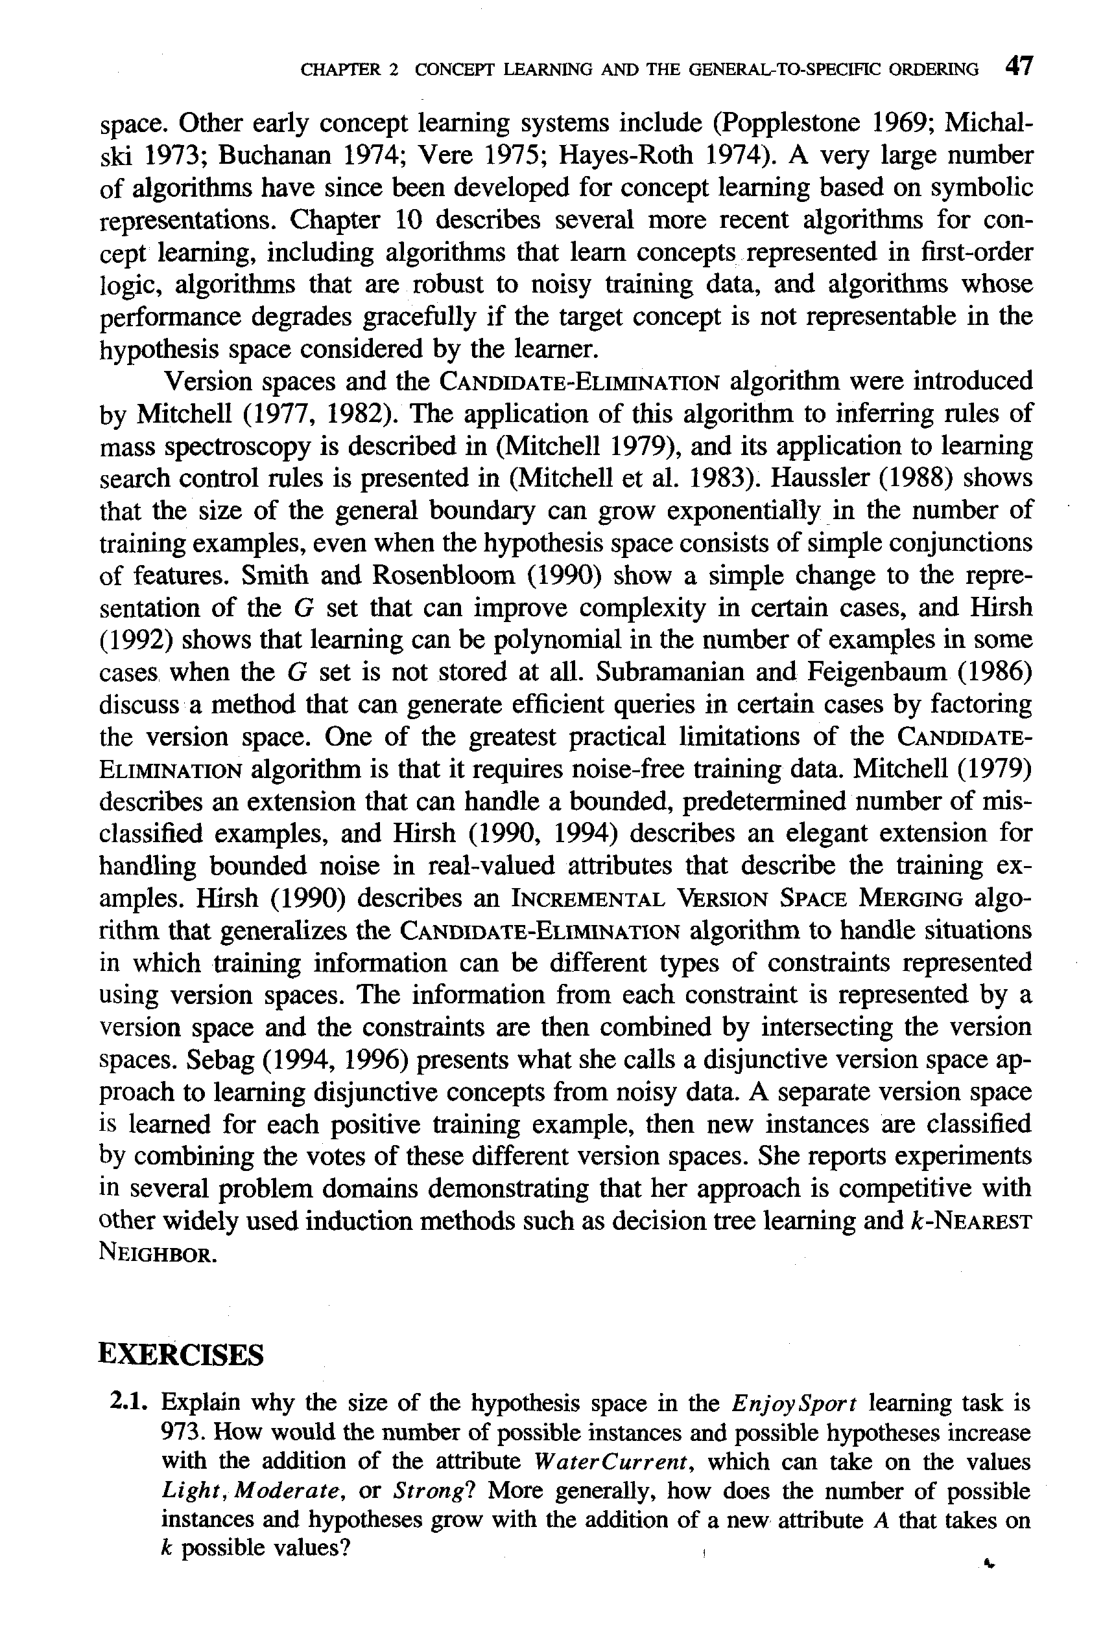
\includegraphics[width=0.9\linewidth]{figures/p59_b0.png}
\end{figure}

\subsection{CHAFTER 2 CONCEPT LEARNING AND THE GENERALTO-SPECIFIC ORDEIUNG 47}

Không gian. Các hệ thống concept learning đầu tiên khác bao gồm (Popplestone 1969; Michalski 1973; Buchanan 1974; Vere 1975; Hayes-Roth 1974). Kể từ đó, một số lượng rất lớn các thuật toán đã được phát triển cho concept learning dựa trên các biểu diễn ký hiệu. Chương 10 mô tả một số thuật toán gần đây hơn cho concept learning, bao gồm các thuật toán tìm hiểu các khái niệm được biểu thị bằng logic bậc nhất, các thuật toán mạnh đối với dữ liệu training nhiễu và các thuật toán có hiệu suất giảm dần nếu khái niệm mục tiêu không thể biểu diễn được trong hypothesis space được người học xem xét.

Thuật toán Version spaces và CANDIDATE-ELIMINATION đã được giới thiệu

Của Mitchell (1977, 1982). Việc áp dụng thuật toán này để suy ra các quy tắc của quang phổ khối được mô tả trong (Mitchell 1979), và ứng dụng của nó để học các quy tắc điều khiển tìm kiếm được trình bày trong (Mitchell và cộng sự 1983). Haussler (1988) chỉ ra rằng kích thước của ranh giới chung có thể tăng theo cấp số nhân theo số lượng mẫu training, ngay cả khi hypothesis space bao gồm các liên kết đơn giản của features. Smith và Rosenbloom (1990) chỉ ra một thay đổi đơn giản trong cách biểu diễn tập G có thể cải thiện độ phức tạp trong một số trường hợp nhất định, và Hirsh (1992) chỉ ra rằng việc học có thể là đa thức về số lượng ví dụ trong một số trường hợp khi tập G không được lưu trữ chút nào. Subramanian và Feigenbaum (1986) thảo luận về một phương pháp có thể tạo ra các truy vấn hiệu quả trong một số trường hợp nhất định bằng cách phân tích version space. Một trong những hạn chế thực tế lớn nhất của thuật toán CANDIDATEELIMINATION là nó yêu cầu dữ liệu training không bị nhiễu. Mitchell (1979)

Mô tả một tiện ích mở rộng có thể xử lý một số lượng mẫu bị classification sai có giới hạn, được xác định trước và Hirsh (1990, 1994) mô tả một tiện ích mở rộng tinh tế để xử lý nhiễu bị chặn trong các thuộc tính có giá trị thực mô tả các ví dụ training. Hirsh (1990) mô tả thuật toán INCREMENTAL VERSION SPACE MERGING

Rithm khái quát hóa thuật toán CANDIDATE-ELIMINATION để xử lý các tình huống

Trong đó thông tin training có thể là các loại ràng buộc khác nhau được biểu diễn bằng version spaces. Thông tin từ mỗi ràng buộc được biểu thị bằng version space và sau đó các ràng buộc này được kết hợp bằng cách giao với version spaces. Sebag (1994, 1996) trình bày cái mà cô gọi là cách tiếp cận version space phân biệt để học các khái niệm phân biệt từ dữ liệu nhiễu. Một version space riêng biệt được học cho mỗi mẫu training tích cực, sau đó các phiên bản mới được phân loại bằng cách kết hợp phiếu bầu của các version spaces khác nhau này. Cô báo cáo các thử nghiệm trong một số lĩnh vực bài toán chứng minh rằng phương pháp của cô có khả năng cạnh tranh với các phương pháp quy nạp được sử dụng rộng rãi khác như decision tree learning và k-NEAREST NEIGHBOR.

\section{EXERCISES}

2.1. Giải thích tại sao kích thước của hypothesis space trong nhiệm vụ học tập EnjoySport lại lớn

973. Số lượng các trường hợp có thể xảy ra và các giả thuyết khả thi sẽ tăng lên như thế nào khi bổ sung thuộc tính Dòng nước, thuộc tính này có thể mang các giá trị Nhẹ, Trung bình hoặc Mạnh? Tổng quát hơn, số lượng trường hợp và giả thuyết có thể tăng lên như thế nào khi bổ sung thuộc tính A mới có k giá trị có thể? , TÔI

% --- page 60 ---
\begin{figure}[ht]
\centering
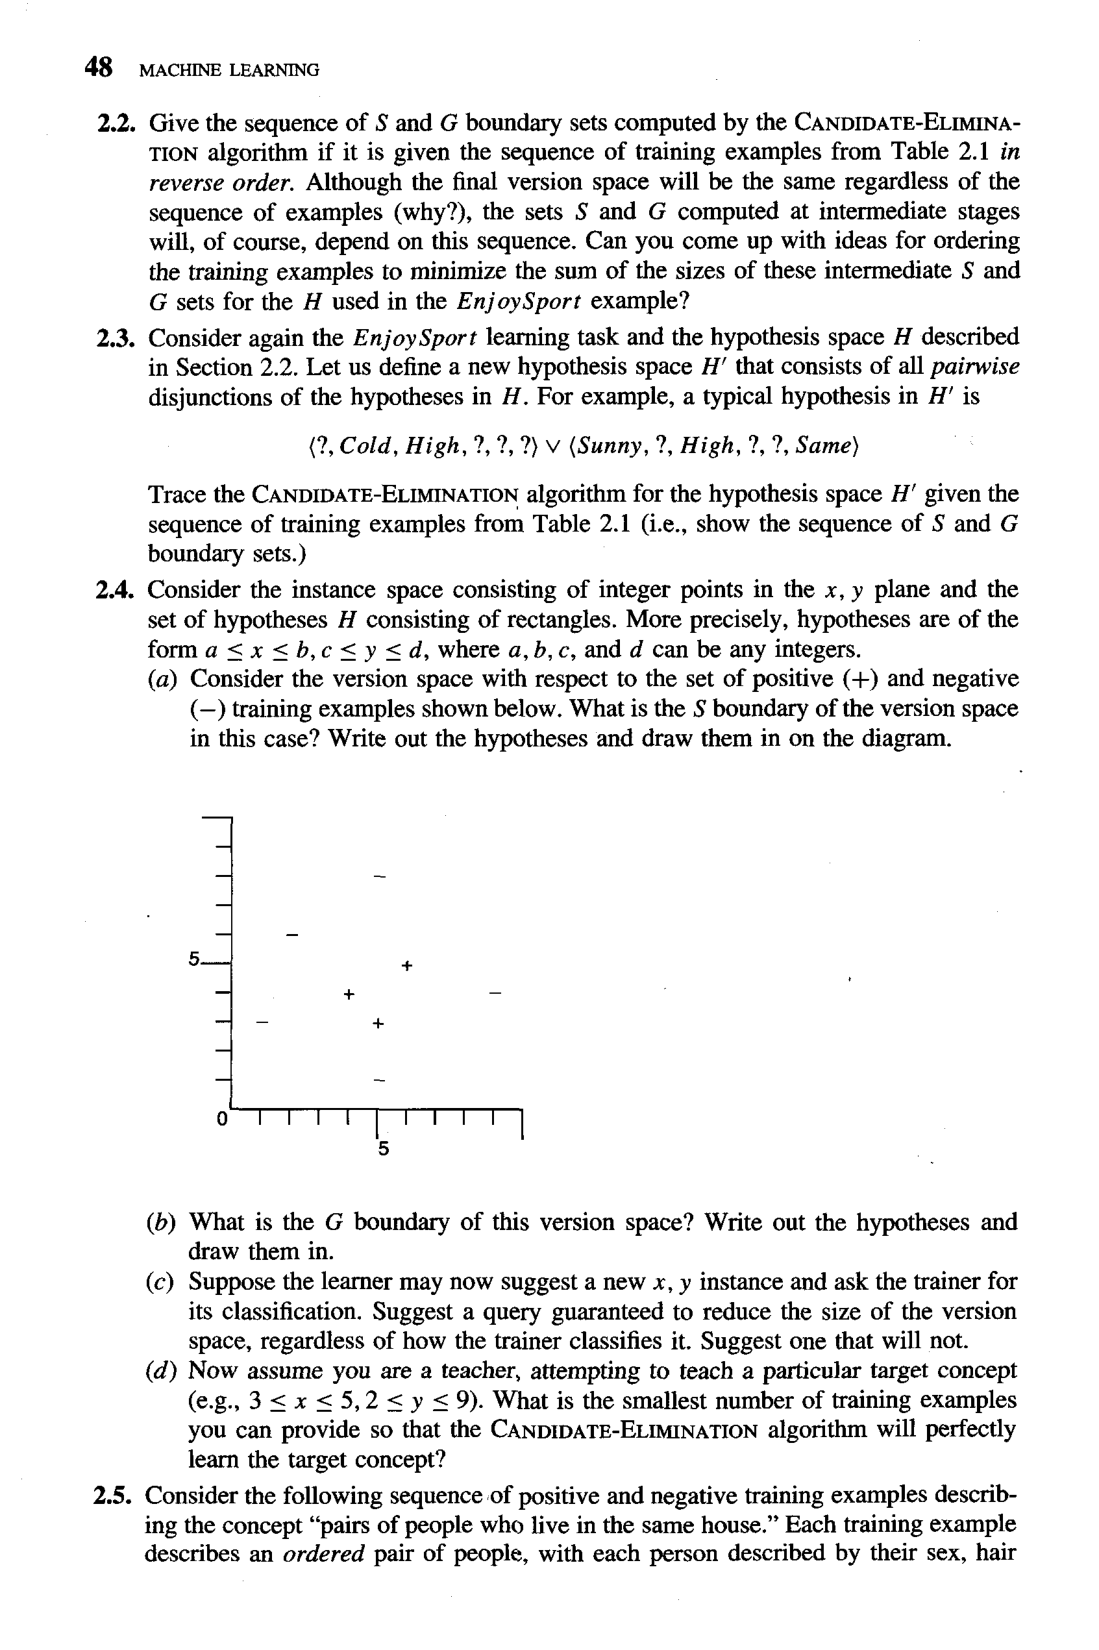
\includegraphics[width=0.9\linewidth]{figures/p60_b0.png}
\end{figure}

2.2. Đưa ra chuỗi các tập ranh giới S và G được tính toán bởi CANDIDATE-ELIMINA-

Thuật toán TION nếu nó được đưa ra chuỗi các ví dụ training từ Bảng 2.1 theo thứ tự ngược lại. Mặc dù version space cuối cùng sẽ giống nhau bất kể trình tự của các ví dụ (tại sao?), tất nhiên, các tập S và G được tính ở các giai đoạn trung gian sẽ phụ thuộc vào trình tự này. Bạn có thể nảy ra ý tưởng sắp xếp thứ tự các ví dụ training để giảm thiểu tổng kích thước của các tập S và G trung gian này cho H được sử dụng trong ví dụ EnjoySport không?

2.3. Xem xét lại nhiệm vụ học tập EnjoySport và hypothesis space H được mô tả

Trong Phần 2.2. Chúng ta hãy định nghĩa một hypothesis space H' mới bao gồm tất cả các điểm khác biệt rõ ràng của các giả thuyết trong H . Ví dụ, một giả thuyết điển hình trong H' là

(?, Lạnh, Cao, ?, ?, ?) v (Nắng, ?, Cao, ?, ?, Tương tự)

Theo dõi thuật toán CANDIDATE-ELIMINATION cho hypothesis space H' cho trước

Chuỗi các ví dụ training từ Bảng 2.1 (tức là hiển thị chuỗi S và G

Tập hợp ranh giới.)

2.4. Xét không gian thể hiện gồm các điểm nguyên trong mặt phẳng x , y và

Tập giả thuyết H gồm các hình chữ nhật. Chính xác hơn, các giả thuyết có dạng a 5 x 5 b, c 5 y 5 d, trong đó a, b, c và d có thể là số nguyên bất kỳ. (a) Xét version space theo tập dương (+) và âm

(-) ví dụ training được hiển thị dưới đây. Ranh giới S của version space trong trường hợp này là gì? Viết ra các giả thuyết và vẽ chúng vào sơ đồ.

(b) Ranh giới G của version space này là gì? Viết ra các giả thuyết và

Kéo chúng vào.

(c) Giả sử bây giờ người học có thể đề xuất một trường hợp x , y mới và yêu cầu người training

Classification của nó. Đề xuất một truy vấn được đảm bảo để giảm kích thước của version space, bất kể người training classification nó như thế nào. Đề nghị một cái sẽ không.

(d) Bây giờ giả sử bạn là một giáo viên, đang cố gắng dạy một khái niệm mục tiêu cụ thể

(ví dụ: 3 5 x 5 5 , 2 ( y 5 9). Bạn có thể cung cấp số lượng mẫu training nhỏ nhất để thuật toán CANDIDATE-ELIMINATION thực hiện hoàn hảo

Tìm hiểu khái niệm mục tiêu?

2.5. Hãy xem xét chuỗi các ví dụ training tích cực và tiêu cực sau đây được mô tả-

Đưa ra khái niệm “những cặp người sống chung một nhà”. Mỗi ví dụ training mô tả một cặp người có thứ tự, mỗi người được mô tả theo giới tính, kiểu tóc

% --- page 61 ---
\begin{figure}[ht]
\centering
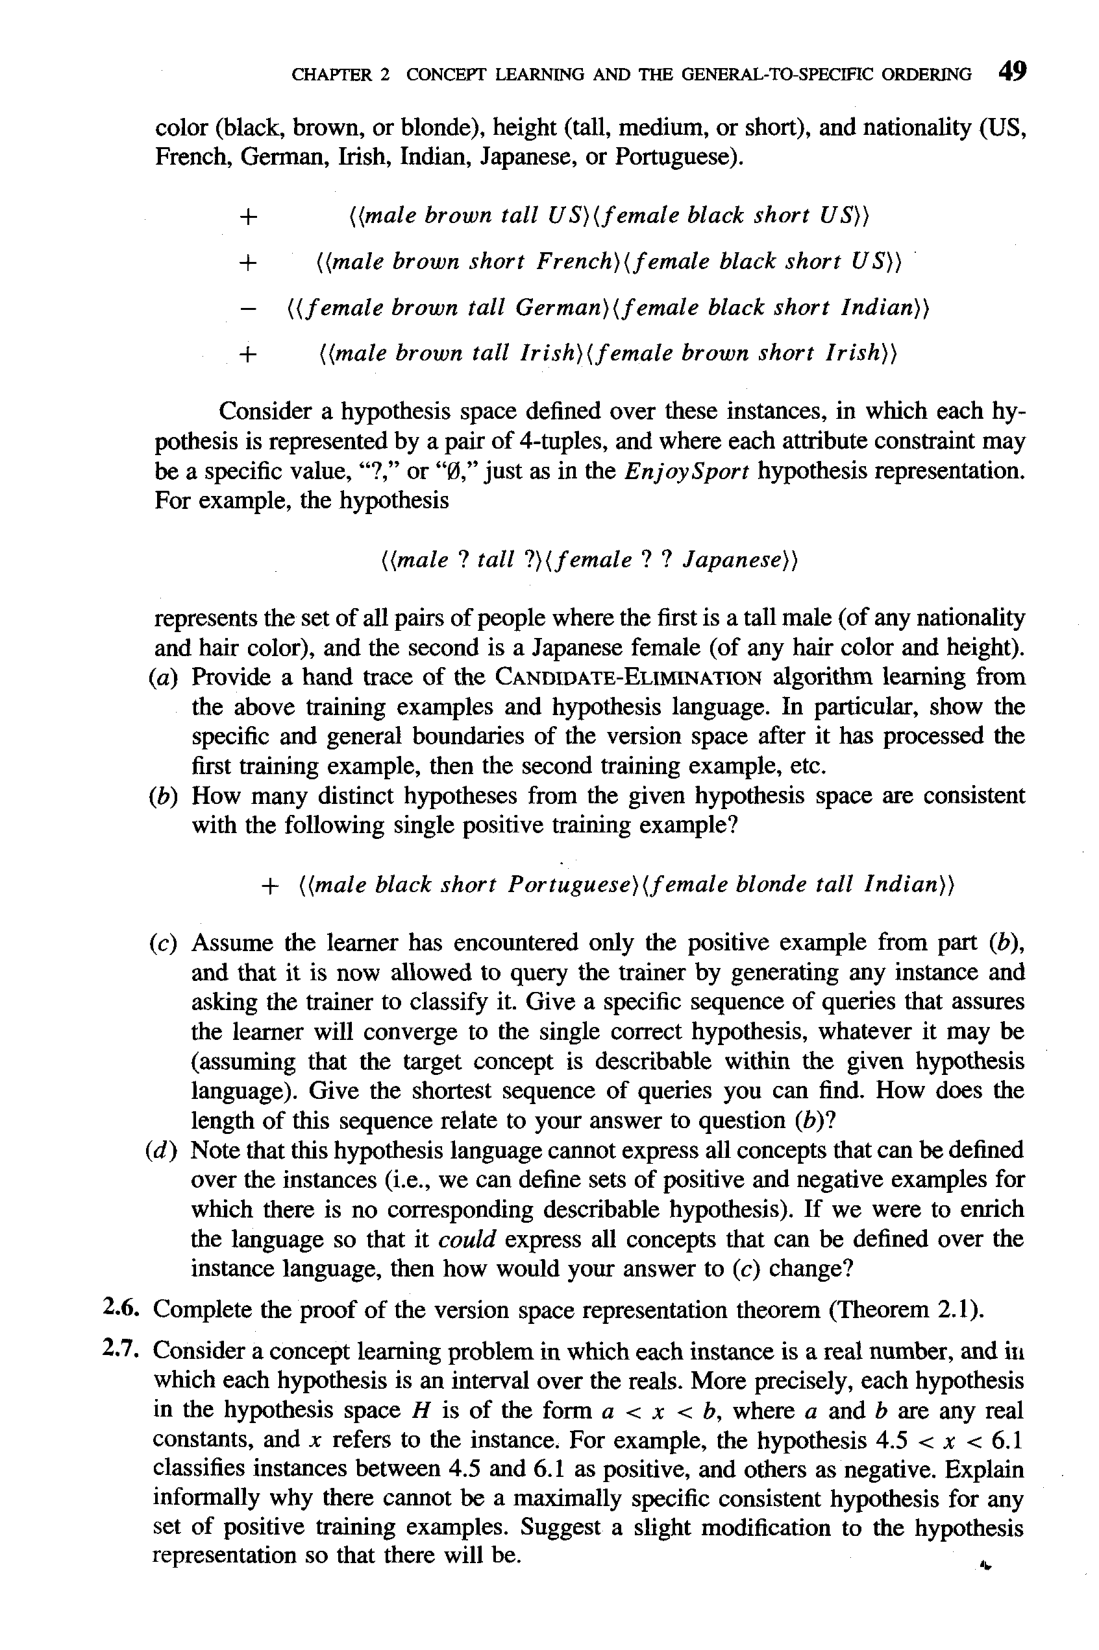
\includegraphics[width=0.9\linewidth]{figures/p61_b0.png}
\end{figure}

\subsection{CHAPTER 2 CONCEPT LEARNING AND THE GENERAL-TO-SPECIFIC ORDERING 49}

Màu sắc (đen, nâu hoặc vàng), chiều cao (cao, trung bình hoặc thấp) và quốc tịch (US, Pháp, Đức, Ireland, Ấn Độ, Nhật Bản hoặc Bồ Đào Nha).

+ ((nam cao màu nâu US) (f nữ thấp màu đen US))

\subsection{+ ((nam ngắn màu nâu Pháp)( nữ ngắn màu đen US))}

- ((nữ người Đức cao màu nâu)( f nữ người da đỏ lùn da đen)) + ((nam người Ireland cao màu nâu) (f nữ người Ireland thấp màu nâu))

Hãy xem xét một hypothesis space được xác định trong các trường hợp này, trong đó mỗi hy-

Giả thuyết được biểu diễn bằng một cặp Ctuples và trong đó mỗi ràng buộc thuộc tính có thể là một giá trị cụ thể, "?," hoặc "0," giống như trong cách biểu diễn giả thuyết EnjoySport. Ví dụ, giả thuyết

((nam ? Cao?)(nữ ? ? Nhật))

Đại diện cho tập hợp tất cả các cặp người trong đó người đầu tiên là nam cao (thuộc mọi quốc tịch và màu tóc) và người thứ hai là nữ Nhật Bản (bất kỳ màu tóc và chiều cao nào).

(a) Cung cấp dấu vết tay của thuật toán CANDIDATE-ELIMINATION học từ

Các ví dụ training và ngôn ngữ giả thuyết ở trên. Cụ thể, hiển thị các ranh giới cụ thể và chung của version space sau khi nó xử lý ví dụ training đầu tiên, sau đó là ví dụ training thứ hai, v.v.

(b) Có bao nhiêu giả thuyết khác biệt từ hypothesis space đã cho là phù hợp

Với ví dụ training tích cực duy nhất sau đây?

\subsection{+ ((nam người Bồ Đào Nha lùn da đen)(f nữ tóc vàng cao người Ấn Độ))}

(c) Giả sử người học chỉ gặp ví dụ tích cực ở phần (b),

Và giờ đây nó được phép truy vấn người training bằng cách tạo ra bất kỳ phiên bản nào và yêu cầu người training classification nó. Đưa ra một chuỗi truy vấn cụ thể để đảm bảo người học sẽ hội tụ đến một giả thuyết chính xác duy nhất, bất kể nó có thể là gì (giả sử rằng khái niệm mục tiêu có thể được mô tả bằng ngôn ngữ giả thuyết đã cho). Đưa ra chuỗi truy vấn ngắn nhất mà bạn có thể tìm thấy. Độ dài của chuỗi này liên quan thế nào đến câu trả lời của bạn cho câu hỏi (b)?

(d) Lưu ý rằng ngôn ngữ giả thuyết này không thể diễn đạt tất cả các khái niệm có thể được định nghĩa

over the instances (i.e., we can define sets of positive and negative examples for which there is no corresponding describable hypothesis). If we were to enrich the language so that it could express all concepts that can be defined over the instance language, then how would your answer to (c) change?

2.6. Hoàn thành chứng minh định lý biểu diễn version space (Định lý 2.1).

Hãy xem xét một bài toán concept learning trong đó mỗi trường hợp là một số thực và trong đó mỗi giả thuyết là một khoảng trên các số thực. Chính xác hơn, mỗi giả thuyết trong hypothesis space H có dạng a < x < b, trong đó a và b là các hằng số thực bất kỳ và x đề cập đến thể hiện. Ví dụ: giả thuyết 4.5 < x < 6.1 classification các trường hợp trong khoảng từ 4,5 đến 6,1 là dương và các trường hợp khác là âm. Giải thích một cách không chính thức lý do tại sao không thể có một giả thuyết nhất quán cụ thể tối đa cho bất kỳ tập hợp ví dụ training tích cực nào. Đề nghị sửa đổi một chút cho giả thuyết

Đại diện nên sẽ có. 'C

% --- page 62 ---
\begin{figure}[ht]
\centering
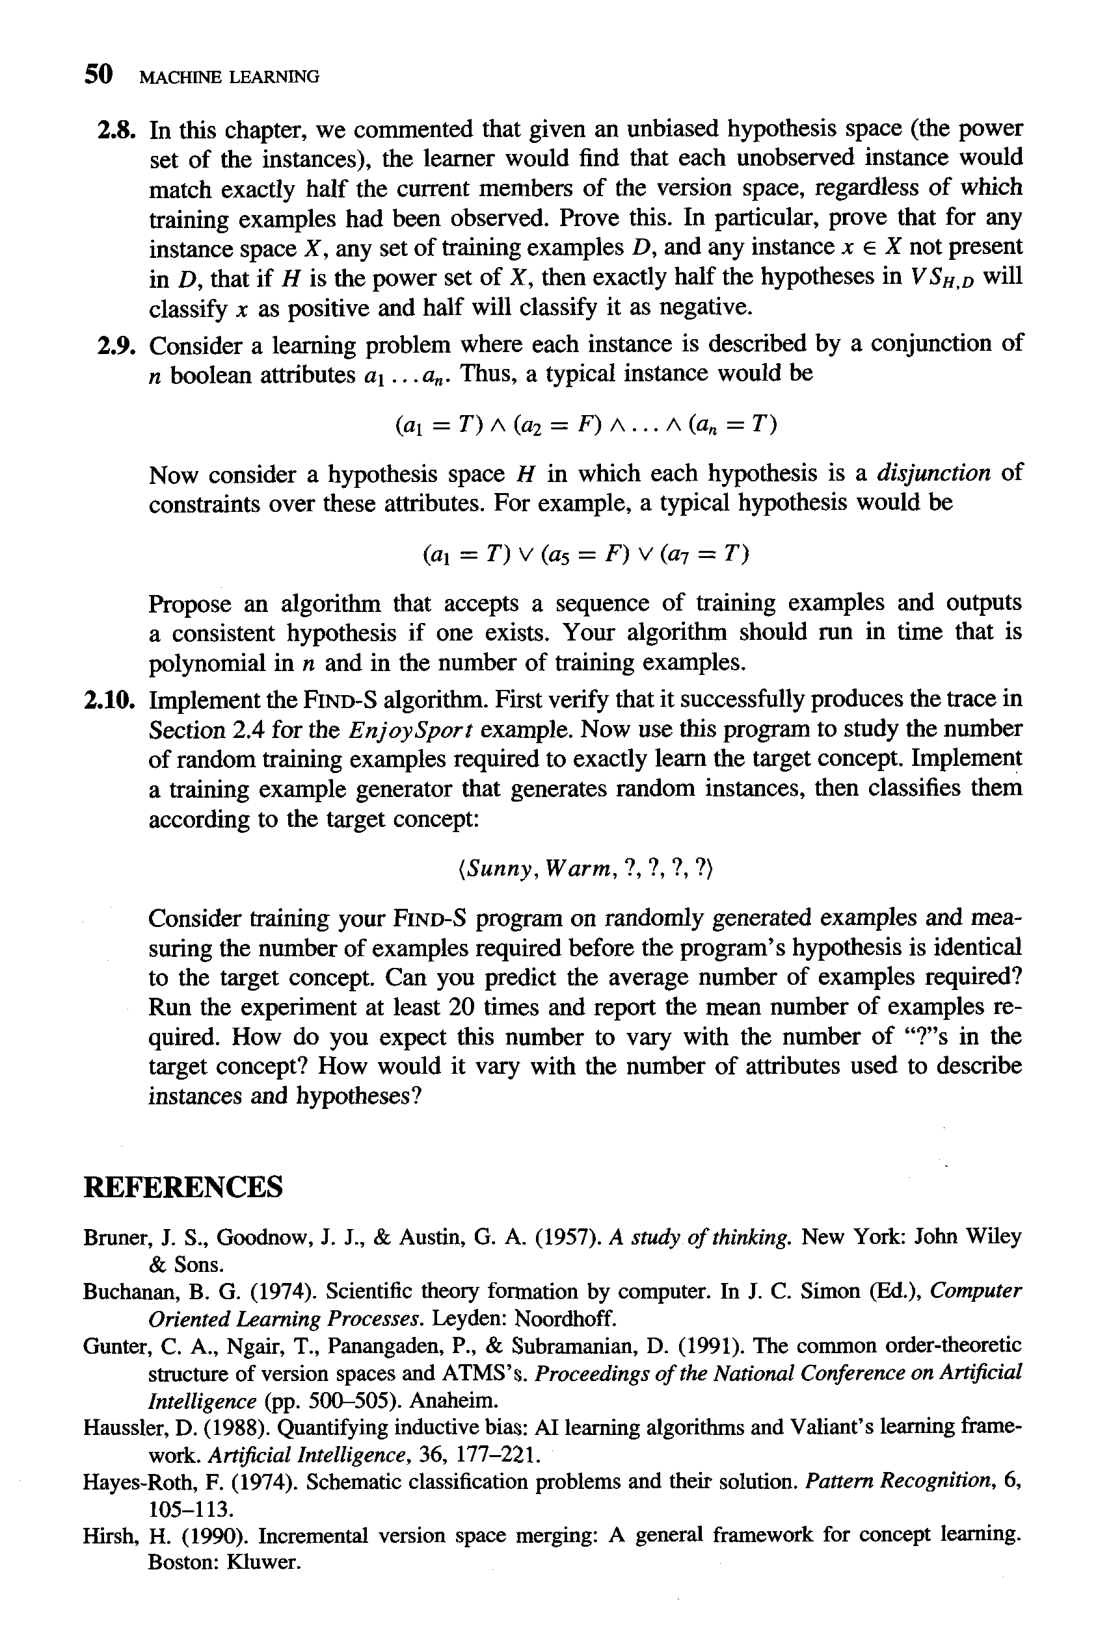
\includegraphics[width=0.9\linewidth]{figures/p62_b0.png}
\end{figure}

\section{MACHINE LEARNING}

2.8. Trong chương này, chúng ta đã nhận xét rằng với hypothesis space không bias (sức mạnh

Tập hợp các trường hợp), người học sẽ thấy rằng mỗi trường hợp không được quan sát sẽ

Khớp chính xác với một nửa số thành viên hiện tại của version space, bất kể ví dụ training nào đã được quan sát. Chứng minh điều này. Cụ thể, chứng minh rằng với mọi version space X, mọi tập mẫu training D và mọi phiên bản x E X không có trong D, rằng nếu H là tập lũy thừa của X thì chính xác một nửa giả thuyết trong VSH,D sẽ classification x là dương và một nửa sẽ classification nó là âm.

2.9. Hãy xem xét một vấn đề học tập trong đó mỗi trường hợp được mô tả bằng sự kết hợp của

N thuộc tính boolean a1 . . .Một,. Vì vậy, một trường hợp điển hình sẽ là

\[(al = T) A (az = F ) A . . . A (a, = T)\]

Bây giờ hãy xem xét hypothesis space H trong đó mỗi giả thuyết là sự phân tách các ràng buộc đối với các thuộc tính này. Ví dụ, một giả thuyết điển hình sẽ là

Đề xuất một thuật toán chấp nhận một chuỗi các ví dụ training và đưa ra một giả thuyết nhất quán nếu có. Thuật toán của bạn phải chạy trong thời gian đa thức tính bằng n và theo số lượng mẫu training.

2.10. Thực hiện thuật toán FIND-S. Trước tiên hãy xác minh rằng nó tạo thành công dấu vết trong

Phần 2.4 về ví dụ về Enjoysport. Bây giờ hãy sử dụng chương trình này để nghiên cứu số lượng ví dụ training ngẫu nhiên cần thiết để tìm hiểu chính xác khái niệm mục tiêu. Triển khai trình tạo ví dụ training để tạo các phiên bản ngẫu nhiên, sau đó classification chúng theo khái niệm đích:

(Nắng, Ấm áp, ?, ?, ?, ?)

Hãy cân nhắc việc training chương trình FIND-S của bạn trên các mẫu được tạo ngẫu nhiên và đo lường số lượng mẫu cần thiết trước khi giả thuyết của chương trình giống với khái niệm mục tiêu. Bạn có thể dự đoán số lượng ví dụ trung bình được yêu cầu không? Chạy thử nghiệm ít nhất 20 lần và báo cáo số lượng ví dụ trung bình được yêu cầu. Bạn mong đợi con số này thay đổi như thế nào theo số "?" trong khái niệm mục tiêu? Nó sẽ thay đổi như thế nào tùy theo số lượng thuộc tính được sử dụng để mô tả các trường hợp và giả thuyết?

\subsection{REFERENCES}

Bruner, J. S., Goodnow, J. J., \& Austin, G. A. (1957). Một nghiên cứu về tư duy. New York: John Wiey

\& Con trai.

Hội trưởng, B. G. (1974). Hình thành lý thuyết khoa học bằng máy tính. Trong J. C. Simon (Ed.), Máy tính

Quá trình học tập có định hướng. Leyden: Noordhoff.

Gunter, C. A., Ngair, T., Panangaden, P., \& Subramanian, D. (1991). Lý thuyết trật tự chung

Cấu trúc của version spaces và ATMS. Kỷ yếu của Hội nghị Quốc gia về Trí tuệ Nhân tạo (trang 500-505). Anaheim.

Haussler, D. (1988). Định lượng inductive bias: Thuật toán học A1 và khung học tập của Valiant-

Công việc. Trí tuệ nhân tạo, 36, 177-221.

Hayes-Roth, F. (1974). Sơ đồ các bài toán classification và cách giải. Nhận dạng mẫu, 6,

% 105-113.
Hirsh, H. (1990). Hợp nhất version space tăng dần: Khung chung cho concept learning.

Boston: Kluwer.

% --- page 63 ---
\begin{figure}[ht]
\centering
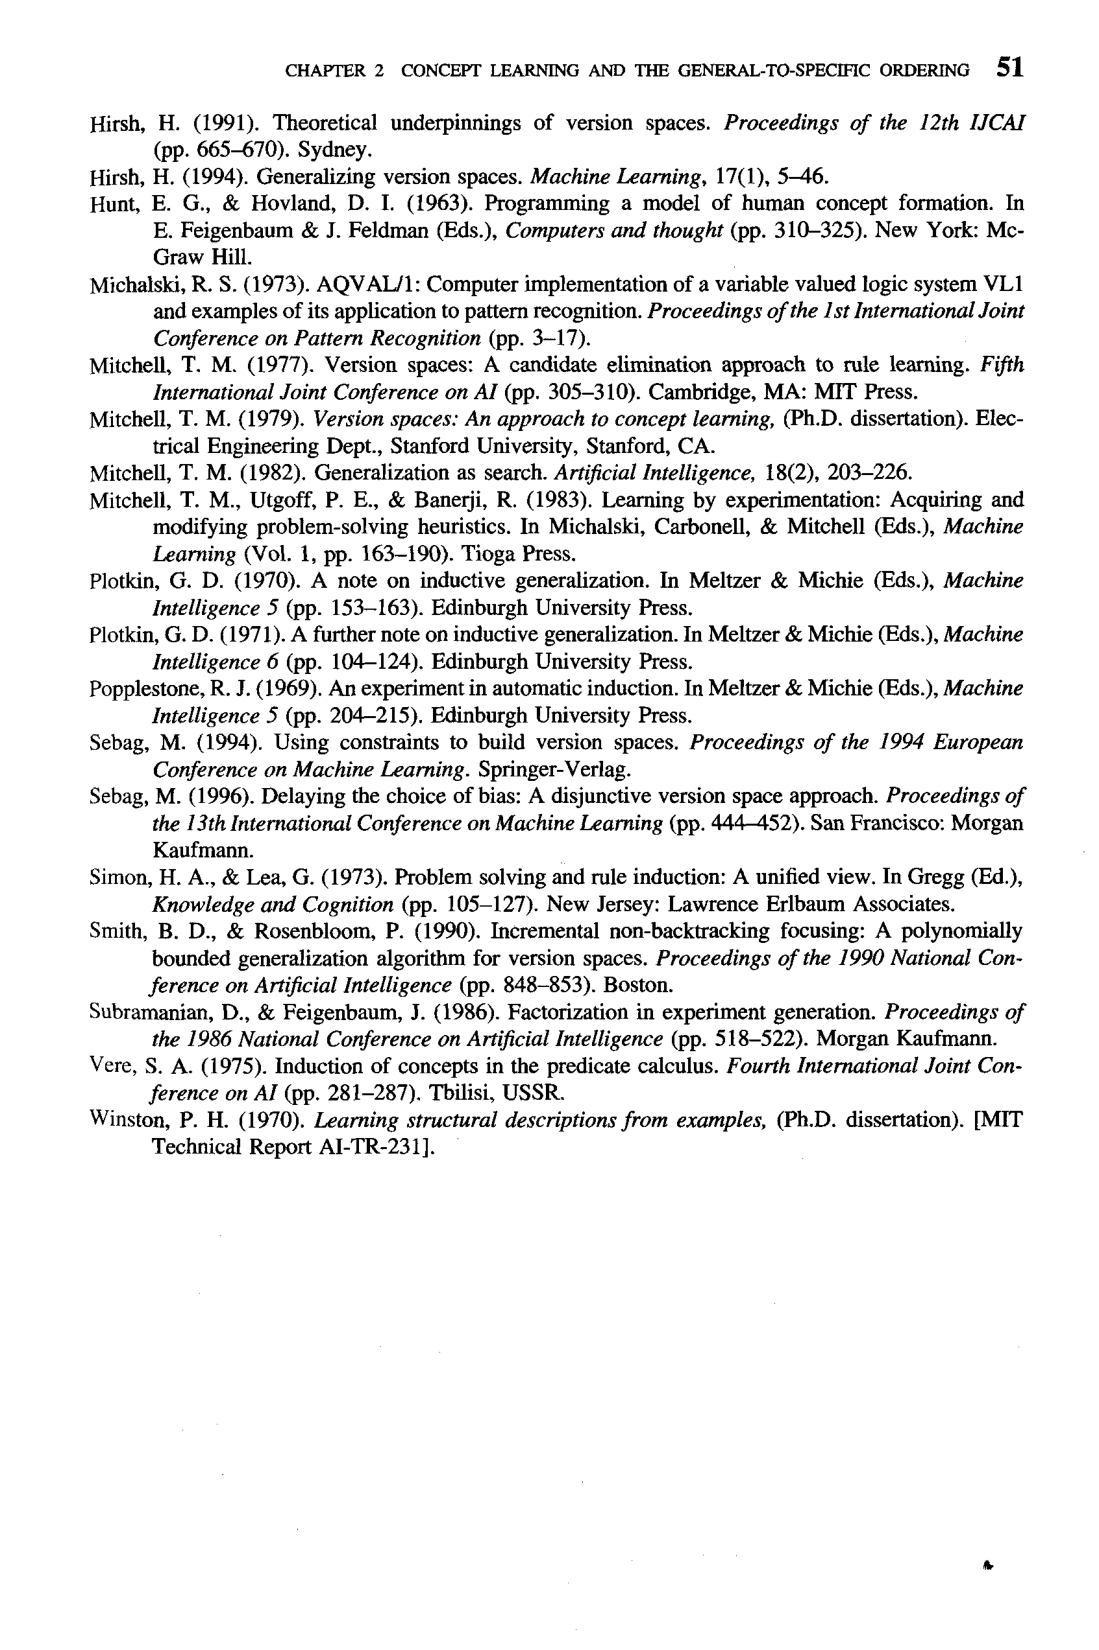
\includegraphics[width=0.9\linewidth]{figures/p63_b0.png}
\end{figure}

Hirsh, H. (1991). Nền tảng lý thuyết của version spaces. Kỷ yếu của IJCAI lần thứ 12

(trang 665-670). Sydney.

Hirsh, H. (1994). Tổng quát hóa version spaces. Machine Learning, 17(1), 546. Hunt, E. G., \& Hovland, D. I. (1963). Lập trình model hình thành khái niệm con người. TRONG

E. Feigenbaum \& J. Feldman (Eds.), Máy tính và tư duy (trang 310-325). New York: Đồi McGraw.

Michalski, R. S. (1973). AQVALI1: Máy tính triển khai hệ thống logic có giá trị thay đổi VL1

Và các ví dụ về ứng dụng của nó vào nhận dạng mẫu. Kỷ yếu của Hội nghị chung quốc tế lần thứ 1 về nhận dạng mẫu (trang 3-17).

Mitchell, TM (1977). Version spaces: Phương pháp loại bỏ ứng viên trong quá trình học quy tắc. Fijlh

Hội nghị chung quốc tế về AI @p. 305-310). Cambridge, MA: Nhà xuất bản MIT.

Mitchell, TM (1979). Version spaces: Cách tiếp cận concept learning, (luận án F'h.D.). Điện-

Khoa Kỹ thuật Trical, Đại học Stanford, Stanford, CA.

Mitchell, TM (1982). Khái quát hóa như tìm kiếm. ArtQcial Tình báo, 18(2), 203-226. Mitchell, T. M., Utgoff, P. E., \& Baneji, R. (1983). Học bằng thử nghiệm: Tiếp thu và

Sửa đổi phương pháp heuristic giải quyết vấn đề. Trong Michalski, Carbonell, \& Mitchell (Eds.), Machine Learning (Tập 1, trang 163-190). Nhà xuất bản Tioga.

Plotkin, GD (1970). Một lưu ý về khái quát hóa quy nạp. Trong Meltzer \& Michie (Biên tập), Máy

Tình báo 5 (trang 153-163). Nhà xuất bản Đại học Edinburgh.

Plotkin, GD (1971). Một lưu ý nữa về khái quát hóa quy nạp. Trong Meltzer \& Michie (Biên tập), Máy

Tình báo 6 (trang 104-124). Nhà xuất bản Đại học Edinburgh.

Popplestone, R. J. (1969). Thí nghiệm về cảm ứng tự động. Trong Meltzer \& Michie (Biên tập), Máy

Tình báo 5 (trang 204-215). Nhà xuất bản Đại học Edinburgh.

Sebag, M. (1994). Sử dụng các ràng buộc để xây dựng version spaces. Kỷ yếu của Hội nghị Châu Âu năm 1994

Hội nghị về Machine Learning. Springer-Verlag.

Sebag, M. (1996). Trì hoãn việc lựa chọn bias: Một cách tiếp cận version space khác biệt. Thủ tục tố tụng của

Hội nghị quốc tế lần thứ 13 về Machine Learning (trang 444-452). San Francisco: Morgan Kaufmann.

Simon, H. A, \& Lea, G. (1973). Giải quyết vấn đề và quy tắc: Một cái nhìn thống nhất. Trong Gregg (Ed.),

Kiến thức và Nhận thức (trang 105-127). New Jersey: Hiệp hội Lawrence Erlbaum.

Smith, B. D., \& Rosenbloom, P. (1990). Lấy nét không quay lại tăng dần: Một đa thức

Thuật toán tổng quát hóa có giới hạn cho version spaces. Kỷ yếu của Hội nghị Quốc gia năm 1990

Tham khảo về ArtQcial Intelligence (trang 848-853). Boston.

Subramanian, D., \& Feigenbaum, J. (1986). Nhân tố hóa trong việc tạo thí nghiệm. Thủ tục tố tụng của

Hội nghị quốc gia I986 về trí thông minh ArtQcial (trang 518-522). Morgan Kaufmann.

Vere, SA (1975). Quy nạp các khái niệm trong phép tính vị từ. Hội nghị chung quốc tế lần thứ tư

Tham khảo về AI (trang 281-287). Tbilisi, USSR.

Winston, P. H. (1970). Học mô tả cấu trúc từ các ví dụ, (luận án tiến sĩ). [MIT

Báo cáo kỹ thuật AI-TR-2311.

% --- page 64 ---
\begin{figure}[ht]
\centering
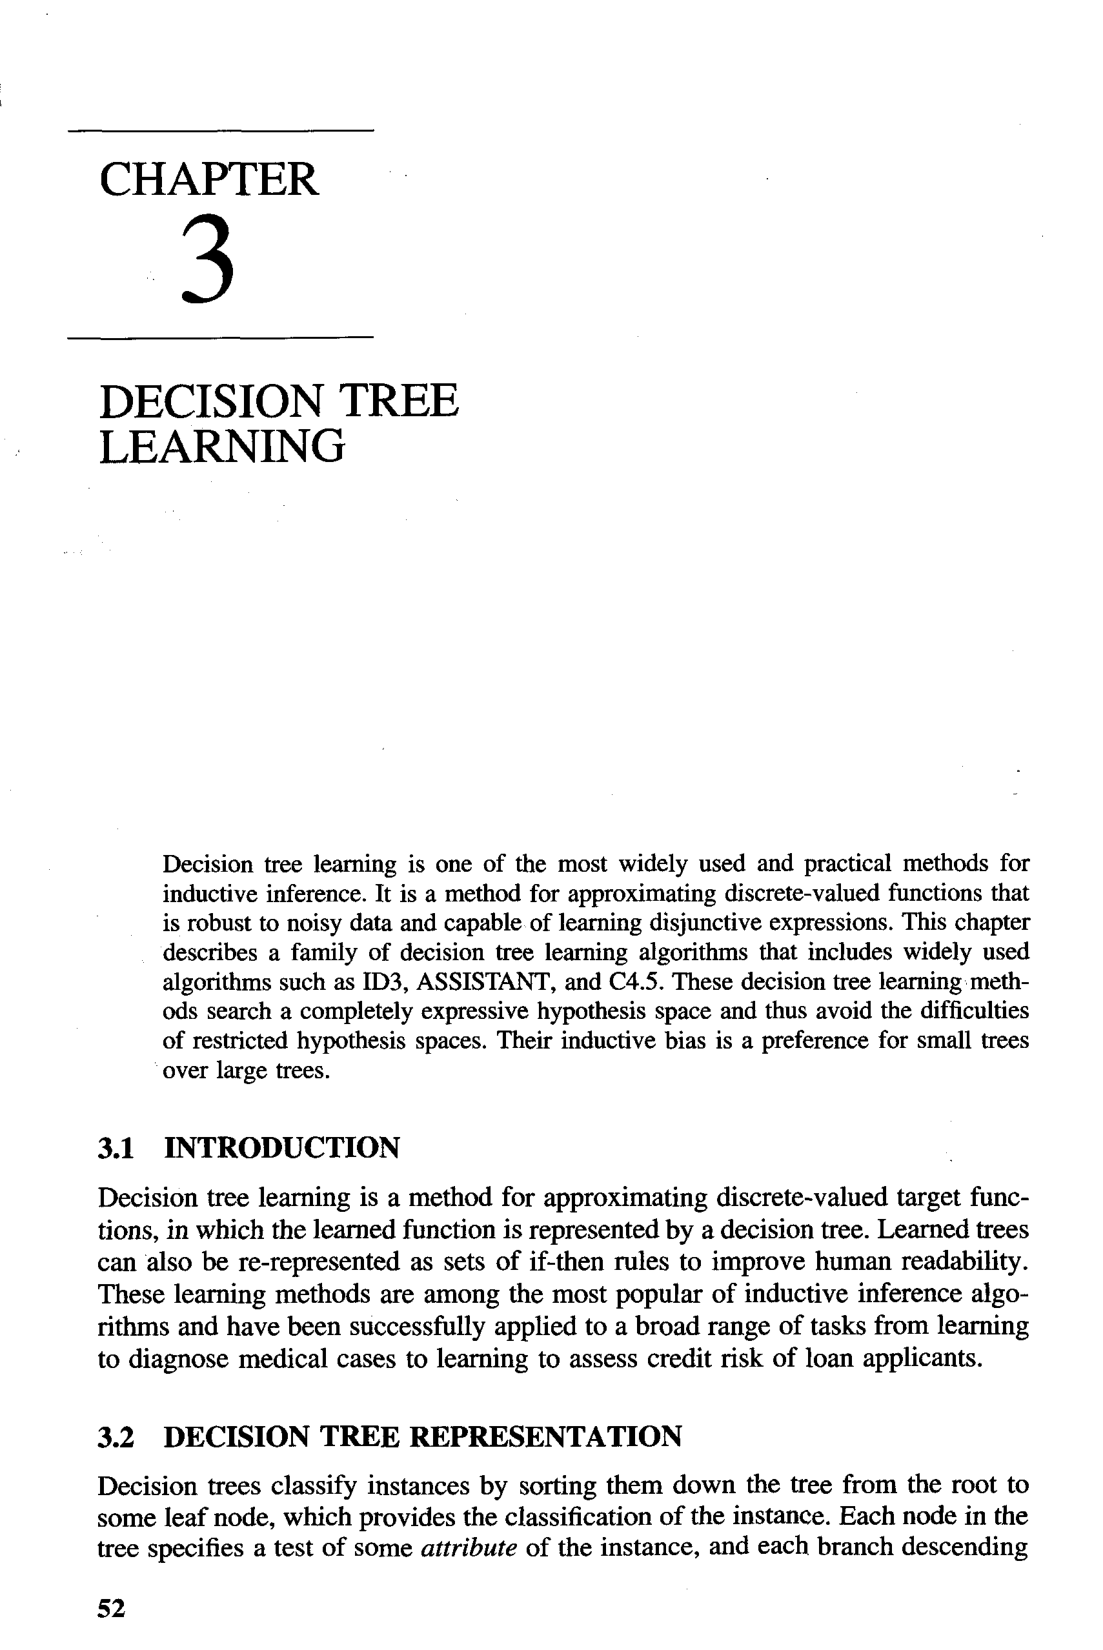
\includegraphics[width=0.9\linewidth]{figures/p64_b0.png}
\end{figure}

\subsection{CHAPTER}

\subsection{DECISION TREE LEARNING}

Decision tree learning là một trong những phương pháp suy luận quy nạp được sử dụng rộng rãi và thiết thực nhất. Đây là một phương pháp xấp xỉ các hàm có giá trị rời rạc, mạnh mẽ đối với dữ liệu nhiễu và có khả năng học các biểu thức phân biệt. Chương này mô tả một họ thuật toán decision tree learning bao gồm các thuật toán được sử dụng rộng rãi như ID3, ASSISTANT và C4.5. Các phương pháp decision tree learning này tìm kiếm hypothesis space hoàn toàn có tính biểu cảm và do đó tránh được những khó khăn của hypothesis spaces bị hạn chế. Inductive bias của họ ưa thích những cây nhỏ hơn những cây lớn.

\subsection{INTRODUCTION}

Decision tree learning là một phương pháp xấp xỉ các hàm mục tiêu có giá trị rời rạc, trong đó hàm đã học được biểu thị bằng decision tree. Cây đã học cũng có thể được biểu diễn lại dưới dạng bộ quy tắc nếu-thì để cải thiện khả năng đọc của con người. Những phương pháp học tập này là một trong những thuật toán suy luận quy nạp phổ biến nhất và đã được áp dụng thành công cho nhiều nhiệm vụ từ học cách chẩn đoán các trường hợp y tế đến học cách đánh giá rủi ro tín dụng của người xin vay.

\subsection{DECISION TREE REPRESENTATION}

Decision trees classification các phiên bản bằng cách sắp xếp chúng theo cây từ gốc đến một số nút lá, cung cấp classification của phiên bản. Mỗi nút trong cây chỉ định việc kiểm tra một số thuộc tính của thể hiện và mỗi nhánh đi xuống

% --- page 65 ---
\begin{figure}[ht]
\centering
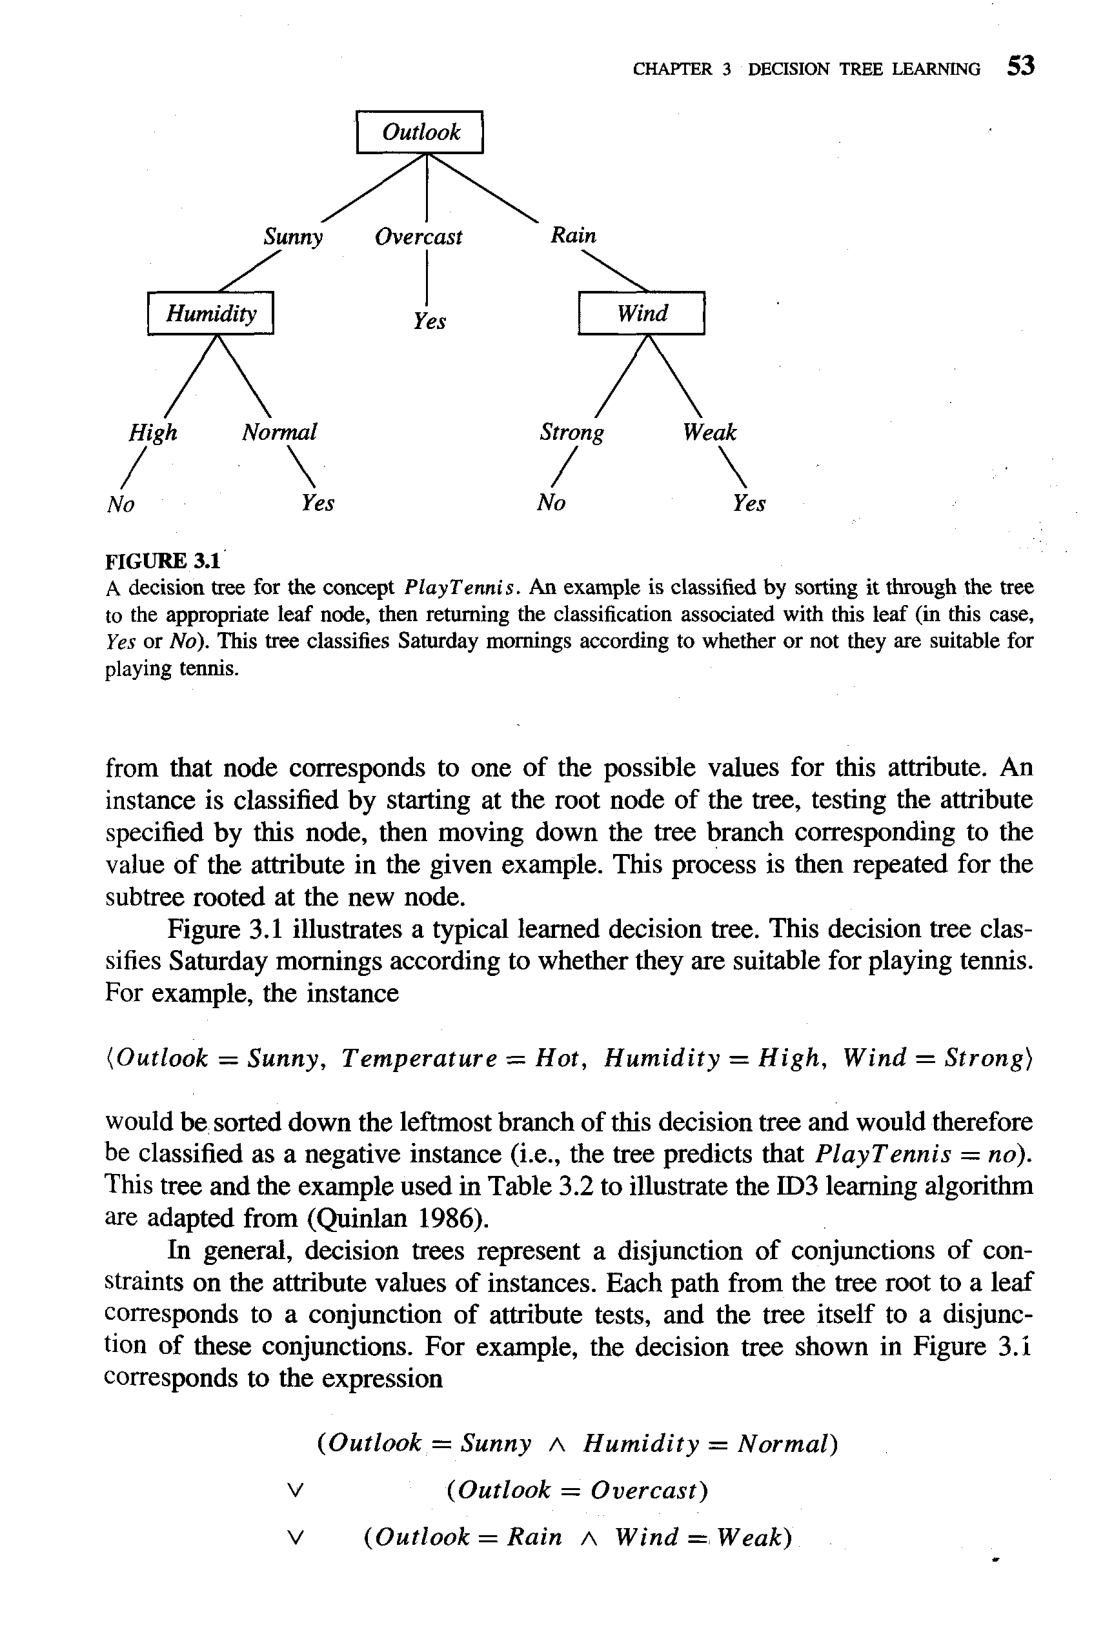
\includegraphics[width=0.9\linewidth]{figures/p65_b0.png}
\end{figure}

\subsection{CHAPTER 3 DECISION TREE LEARNING 53}

\subsection{Noma1 Mạnh Yếu}

\[No \\]

\subsection{Đúng /}

\[No \\]

\subsection{Đúng}

\noindent\textit{FIGURE 3.1 A decision tree cho khái niệm PlayTennis. Một ví dụ được phân loại bằng cách sắp xếp nó qua cây đến nút lá thích hợp, sau đó trả về classification được liên kết với lá này (trong trường hợp này là}

Có hoặc Không). Cây này classification các buổi sáng thứ Bảy theo thời gian có phù hợp hay không.

Chơi quần vợt.

Từ nút đó tương ứng với một trong các giá trị có thể có của thuộc tính này. Một thể hiện được phân loại bằng cách bắt đầu từ nút gốc của cây, kiểm tra thuộc tính được chỉ định bởi nút này, sau đó di chuyển xuống nhánh cây tương ứng với giá trị của thuộc tính trong ví dụ đã cho. Quá trình này sau đó được lặp lại cho cây con có gốc tại nút mới.

\noindent\textit{Hình 3.1 minh họa một decision tree đã học điển hình. Lớp decision tree này-}

Classification các buổi sáng thứ Bảy tùy theo thời điểm thích hợp để chơi quần vợt.

\subsection{Ví dụ, ví dụ}

\[(Outlook = Sunny, Temperature = Hot, Humidity = High, Wind = Strong)\]

Sẽ được sắp xếp theo nhánh ngoài cùng bên trái của decision tree này và do đó sẽ

Được được phân loại là một trường hợp phủ định (tức là cây dự đoán rằng PlayTennis = no). Cây này và ví dụ được sử dụng trong Bảng 3.2 để minh họa thuật toán học ID3 được phỏng theo (Quinlan 1986).

Nói chung, decision trees đại diện cho sự tách rời các liên từ của con-

Căng thẳng về các giá trị thuộc tính của các thể hiện. Mỗi đường dẫn từ gốc cây đến lá tương ứng với sự kết hợp của các phép kiểm tra thuộc tính và bản thân cây tương ứng với sự phân tách của các kết hợp này. Ví dụ: decision tree hiển thị trong Hình 3.1 tương ứng với biểu thức

\[(Outlook = Sunny A Humidity = Normal)\]

\[V (Outlook = Overcast)\]

\[v (Outlook = Rain A Wind = Weak)\]

% --- page 66 ---
\begin{figure}[ht]
\centering
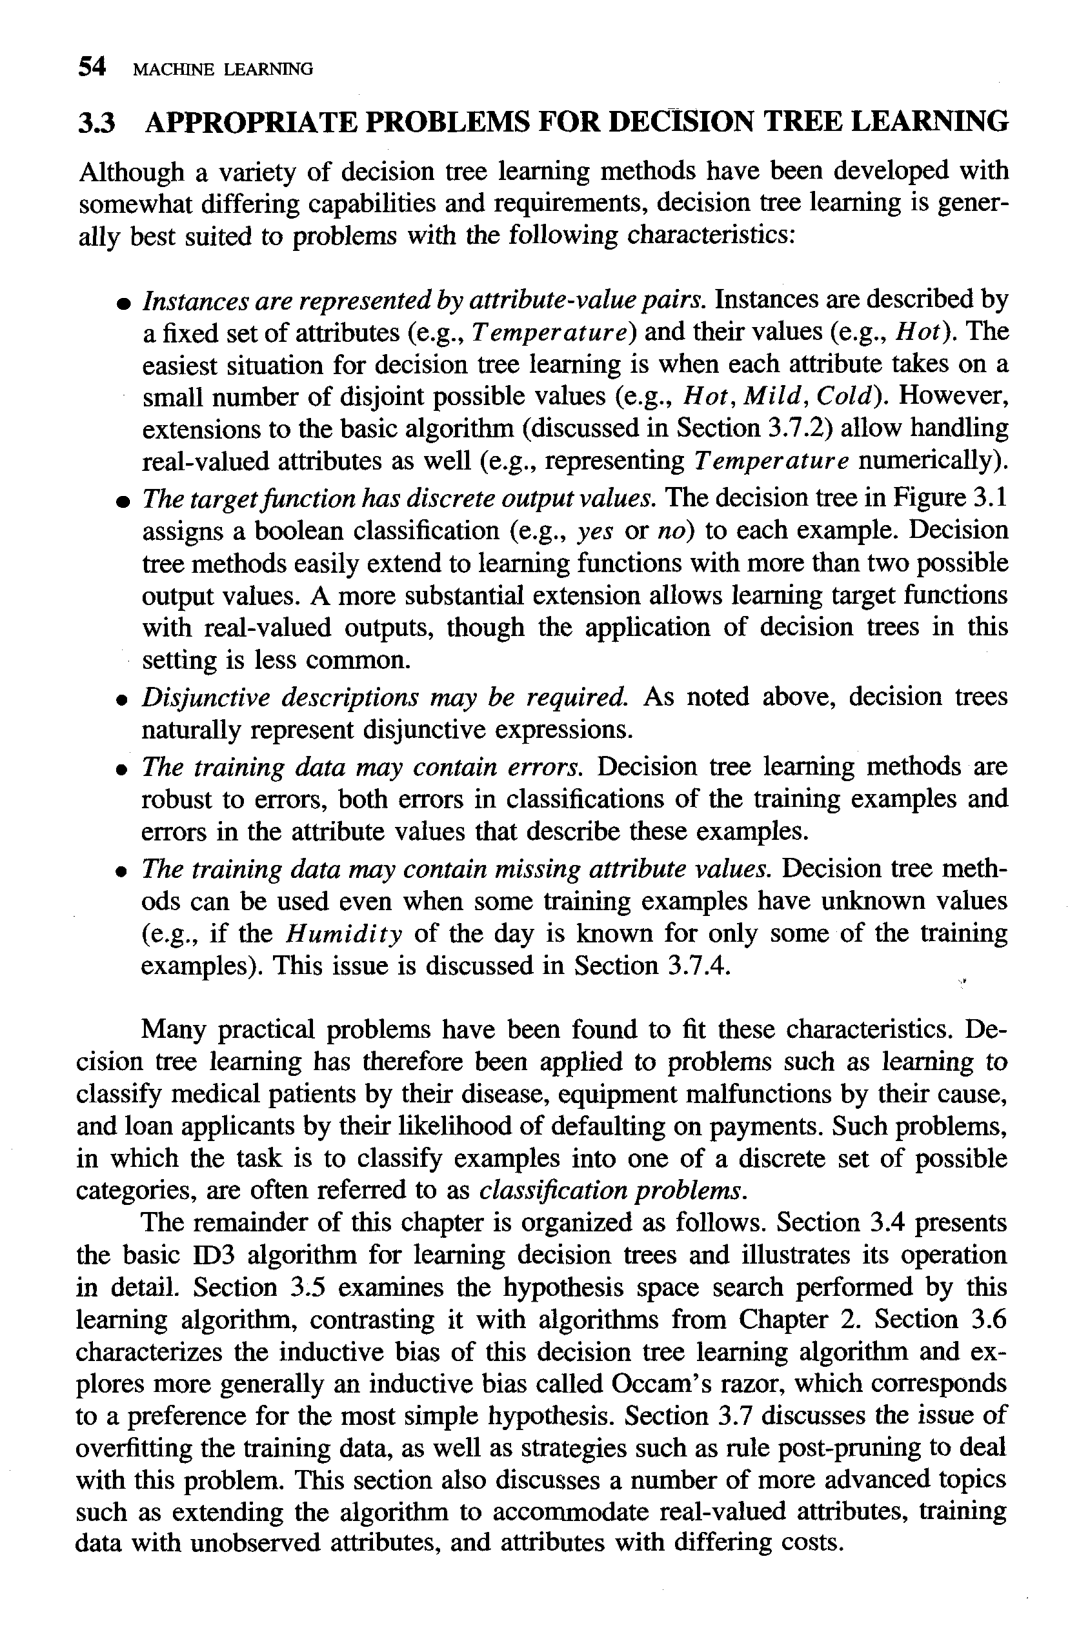
\includegraphics[width=0.9\linewidth]{figures/p66_b0.png}
\end{figure}

\section{MACHINE LEARNWG}

\subsection{APPROPRIATE PROBLEMS FOR DECISION TREE LEARNING}

Mặc dù nhiều phương pháp decision tree learning đã được phát triển với các khả năng và yêu cầu hơi khác nhau, nhưng decision tree learning nhìn chung phù hợp nhất với các bài toán có các đặc điểm sau:

Các thể hiện Zn được biểu diễn bằng các cặp giá trị-thuộc tính. Các trường hợp được mô tả bởi

Một tập hợp các thuộc tính cố định (ví dụ: Nhiệt độ) và các giá trị của chúng (ví dụ: Nóng). Các

Tình huống dễ dàng nhất đối với decision tree learning là khi mỗi thuộc tính đảm nhận một

Số lượng nhỏ các giá trị có thể rời rạc (ví dụ: Nóng, Nhẹ, Lạnh). Tuy nhiên, phần mở rộng của thuật toán cơ bản (được thảo luận trong Phần 3.7.2) cho phép xử lý

Các thuộc tính có giá trị thực (ví dụ: biểu thị Nhiệt độ bằng số).

Hàm mục tiêu có các giá trị đầu ra rời rạc. Decision tree trong Hình 3.1 gán classification boolean (ví dụ: có hoặc không) cho mỗi ví dụ. Các phương pháp Decision tree dễ dàng mở rộng sang các hàm học với nhiều hơn hai giá trị đầu ra có thể. Một phần mở rộng quan trọng hơn cho phép học các hàm mục tiêu với đầu ra có giá trị thực, mặc dù việc áp dụng decision trees trong cài đặt này ít phổ biến hơn.

\section{Có thể cần phải có những mô tả rời rạc. Như đã lưu ý ở trên, decision trees}

Biểu diễn các biểu thức phân biệt một cách tự nhiên.

\section{Dữ liệu training có thể có lỗi. Các phương pháp Decision tree learning là}

Mạnh mẽ đối với các lỗi, cả lỗi trong việc classification các ví dụ training và lỗi trong các giá trị thuộc tính mô tả các ví dụ này.

\section{Dữ liệu training có thể chứa các giá trị thuộc tính bị thiếu. Phương pháp Decision tree-}

Ods có thể được sử dụng ngay cả khi một số ví dụ training có giá trị không xác định (ví dụ: nếu Độ ẩm trong ngày chỉ được biết đối với một số training

Ví dụ). Vấn đề này được thảo luận trong Phần 3.7.4.

Nhiều bài toán thực tế đã được tìm thấy phù hợp với những đặc điểm này. De-

Do đó, học cây cắt đã được áp dụng cho các vấn đề như học cách classification bệnh nhân y tế theo bệnh của họ, trục trặc thiết bị theo nguyên nhân và người xin vay theo khả năng không trả được nợ. Những bài toán như vậy, trong đó nhiệm vụ là classification các ví dụ thành một trong các tập hợp riêng biệt các loại có thể có, thường được gọi là các bài toán classification.

Phần còn lại của chương này được tổ chức như sau. Mục 3.4 trình bày

Thuật toán ID3 cơ bản để học decision trees và minh họa chi tiết hoạt động của nó. Phần 3.5 xem xét tìm kiếm hypothesis space được thực hiện bởi thuật toán học này, đối chiếu nó với các thuật toán từ Chương 2. Phần 3.6 mô tả đặc điểm inductive bias của thuật toán decision tree learning này và khám phá tổng quát hơn một inductive bias được gọi là dao cạo Occam, tương ứng với sở thích dành cho giả thuyết đơn giản nhất. Phần 3.7 thảo luận về vấn đề overfitting, dữ liệu training, cũng như các chiến lược như cắt tỉa quy tắc để giải quyết vấn đề này. Phần này cũng thảo luận về một số chủ đề nâng cao hơn như mở rộng thuật toán để chứa các thuộc tính có giá trị thực, training

Dữ liệu với các thuộc tính không được quan sát và các thuộc tính có chi phí khác nhau.

% --- page 67 ---
\begin{figure}[ht]
\centering
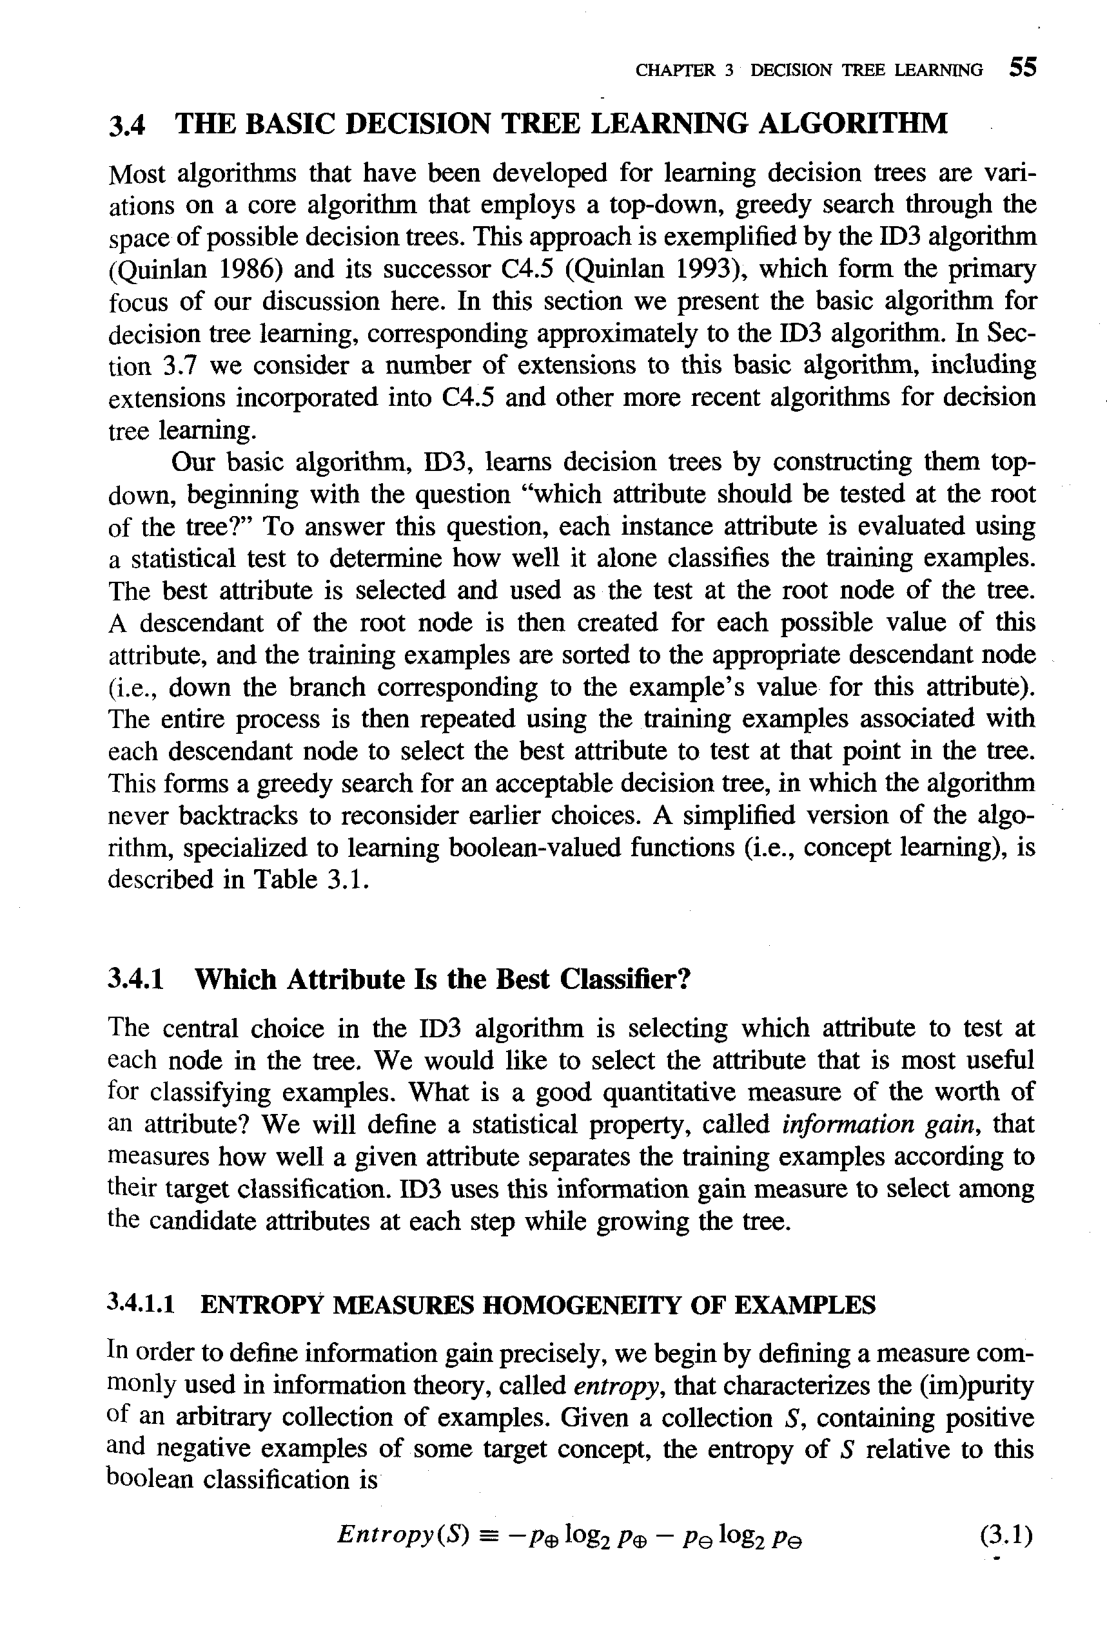
\includegraphics[width=0.9\linewidth]{figures/p67_b0.png}
\end{figure}

\subsection{CHAPTER 3 DECISION TREE LEARMNG 55}

\subsection{THE BASIC DECISION TREE LEARNING ALGORITHM}

Hầu hết các thuật toán đã được phát triển để học decision trees là các biến thể của thuật toán cốt lõi sử dụng tìm kiếm tham lam, từ trên xuống trong không gian có thể có của decision trees. Cách tiếp cận này được minh họa bằng thuật toán ID3 (Quinlan 1986) và thuật toán kế nhiệm C4.5 (Quinlan 1993), đây là trọng tâm chính của cuộc thảo luận của chúng ta ở đây. Trong phần này chúng ta trình bày thuật toán cơ bản cho decision tree learning, tương ứng gần đúng với thuật toán ID3. Trong Phần 3.7, chúng ta xem xét một số phần mở rộng cho thuật toán cơ bản này, bao gồm các phần mở rộng được tích hợp vào C4.5 và các thuật toán khác gần đây hơn cho decision tree learning.

Thuật toán cơ bản của chúng ta, ID3, học decision trees bằng cách xây dựng chúng

Xuống, bắt đầu bằng câu hỏi "thuộc tính nào nên được kiểm tra ở gốc của cây?" Để trả lời câu hỏi này, mỗi thuộc tính individual được đánh giá bằng cách sử dụng một bài kiểm tra thống kê để xác định xem nó classification các ví dụ training tốt như thế nào. Thuộc tính tốt nhất được chọn và sử dụng làm bài kiểm tra ở nút gốc của cây. Sau đó, hậu duệ của nút gốc được tạo cho mỗi giá trị có thể có của thuộc tính này

Thuộc tính và các mẫu training được sắp xếp theo nút con thích hợp (tức là xuống nhánh tương ứng với giá trị của mẫu cho thuộc tính này).

Sau đó, toàn bộ quá trình được lặp lại bằng cách sử dụng các ví dụ training được liên kết với từng nút con để chọn thuộc tính tốt nhất để kiểm tra tại điểm đó trong cây. Điều này tạo thành một cuộc tìm kiếm tham lam cho một decision tree có thể chấp nhận được, trong đó thuật toán không bao giờ quay lại để xem xét lại các lựa chọn trước đó. Một phiên bản đơn giản của thuật toán, chuyên dùng để học các hàm có giá trị boolean (tức là concept learning), được mô tả trong Bảng 3.1.

\subsubsection{Thuộc tính nào là classification tốt nhất?}

Lựa chọn trọng tâm trong thuật toán ID3 là chọn thuộc tính nào để kiểm tra tại mỗi nút trong cây. Chúng ta muốn chọn thuộc tính hữu ích nhất để classification các ví dụ. Một thước đo định lượng tốt về giá trị của một thuộc tính là gì? Chúng ta sẽ xác định một thuộc tính thống kê, được gọi là mức tăng thông tin, đo lường mức độ phân tách của một thuộc tính nhất định giữa các mẫu training theo classification mục tiêu của chúng. ID3 sử dụng thước đo thu được thông tin này để chọn trong số các thuộc tính ứng cử viên ở mỗi bước trong khi phát triển cây.

3.4.1.1 ENTROPY MEASURES HOMOGENEITY OF EXAMPLES

Để xác định độ lợi thông tin một cách chính xác, chúng ta bắt đầu bằng việc định nghĩa một thước đo thường được sử dụng trong lý thuyết thông tin, được gọi là entropy, feature cho độ thuần khiết (không) của một tập hợp các ví dụ tùy ý. Cho một tập hợp S, chứa các ví dụ tích cực và tiêu cực của một số khái niệm mục tiêu, entropy của S liên quan đến điều này

\subsection{Boolean được phân loại là}

% --- page 68 ---
\begin{figure}[ht]
\centering
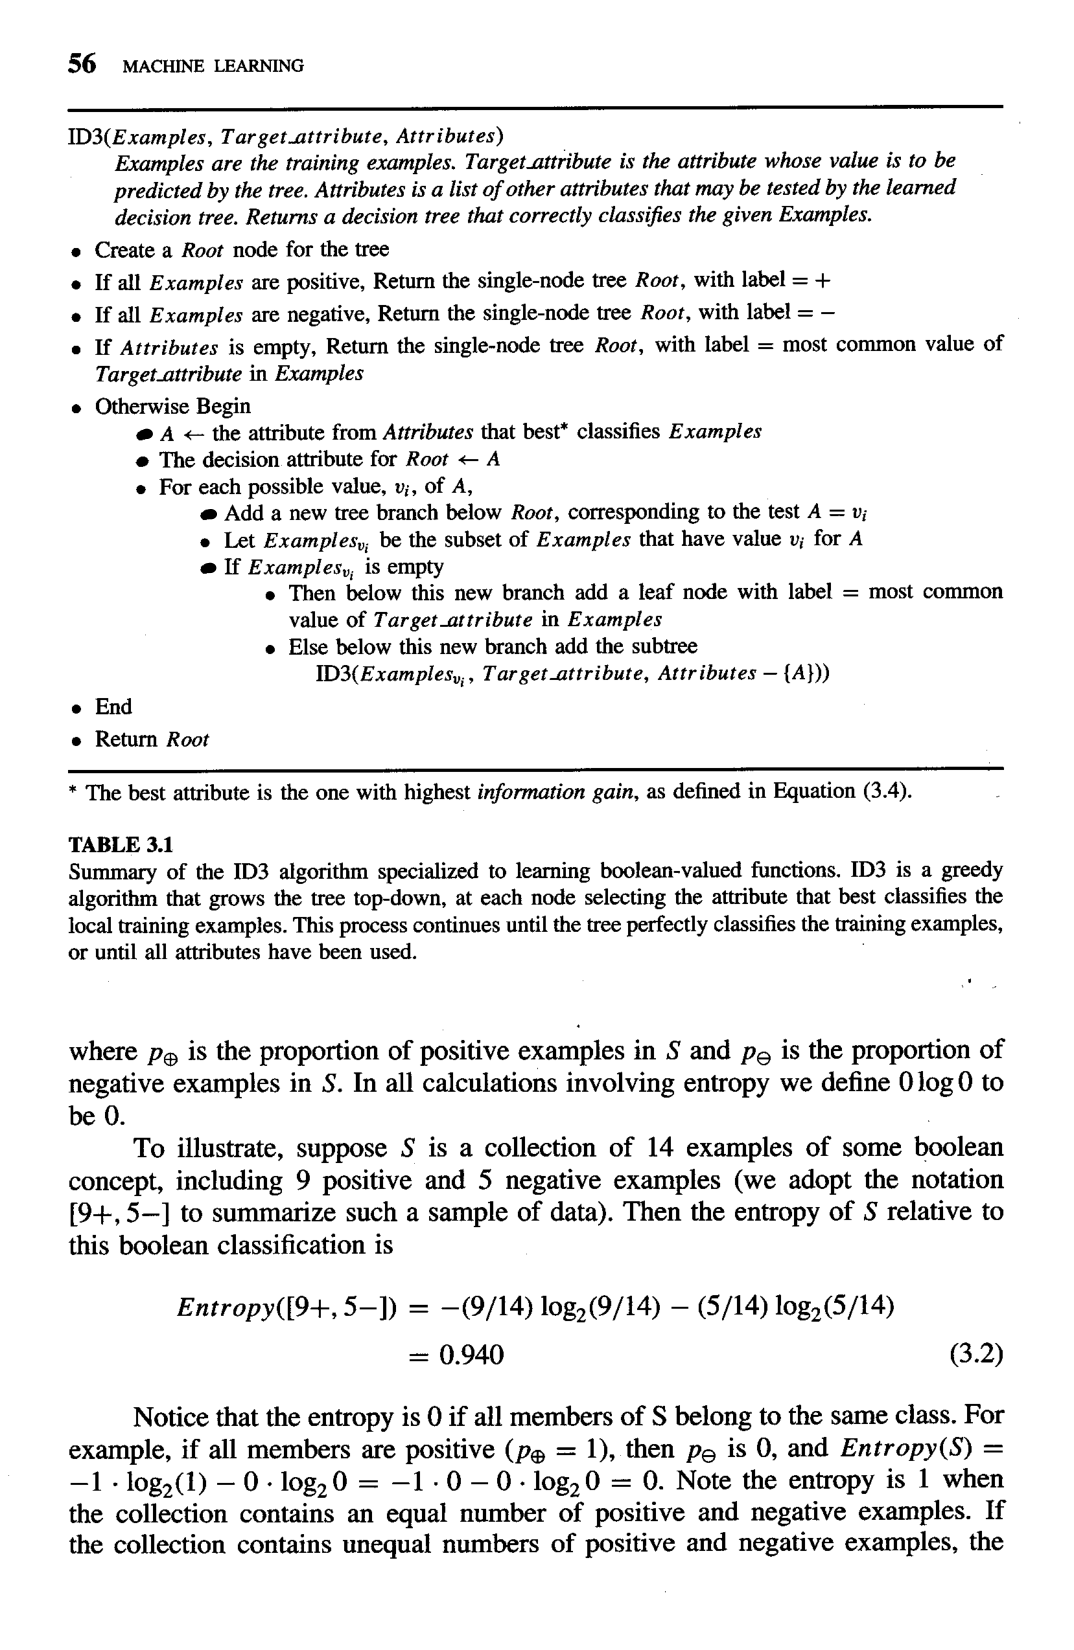
\includegraphics[width=0.9\linewidth]{figures/p68_b0.png}
\end{figure}

ID3(Ví dụ, Thuộc tính mục tiêu, Thuộc tính)

Ví dụ là các ví dụ training. Thuộc tính đích là thuộc tính có giá trị

Dự đoán của cây. Thuộc tính là danh sách các thuộc tính khác có thể được kiểm tra bởi người học

Decision tree. Trả về decision tree classification chính xác các Ví dụ đã cho.

Tạo nút gốc cho cây

\[I f all Examples are positive, Return the single-node tree Root, with label = +\]

\[I f all Examples are negative, Return the single-node tree Root, with label = -\]

Nếu Thuộc tính trống, Trả về Gốc cây nút đơn, với nhãn = giá trị chung nhất của

Thuộc tính mục tiêu trong ví dụ nếu không thì bắt đầu

Thuộc tính từ Thuộc tính* classification tốt nhất Ví dụ

\section{Thuộc tính quyết định cho Root c A}

Với mỗi giá trị có thể có, vi của A,

\[Add a new tree branch below Root, corresponding to the test A = vi\]

\section{Đặt Ví dụ là tập con của Ví dụ có giá trị vi cho A}

Nếu Ví dụ, trống

Sau đó bên dưới nhánh mới này thêm một nút lá có nhãn = giá trị phổ biến nhất của thuộc tính Target trong Ví dụ. Khác bên dưới nhánh mới này thêm cây con

\subsection{ID3(Ví dụ,,, Thuộc tính mục tiêu, Thuộc tính - (A)))}

Kết thúc Trả về gốc

* Thuộc tính tốt nhất là thuộc tính có mức tăng thông tin cao nhất, như được định nghĩa trong Phương trình (3.4).

\noindent\textit{TABLE 3.1 Tóm tắt thuật toán ID3 chuyên dùng để học các hàm có giá trị boolean. ID3 là một thuật toán tham lam phát triển cây từ trên xuống, tại mỗi nút chọn thuộc tính classification tốt nhất các ví dụ training cục bộ. Quá trình này tiếp tục cho đến khi cây classification hoàn hảo các mẫu training hoặc cho đến khi tất cả các thuộc tính đã được sử dụng.}

Trong đó p, là tỷ lệ của các mẫu dương trong S và p, là tỷ lệ của các mẫu âm trong S. Trong tất cả các phép tính liên quan đến entropy, chúng ta xác định 0 log 0 là 0.

Để minh họa, giả sử S là một tập hợp gồm 14 ví dụ về một số boolean

Khái niệm, bao gồm 9 ví dụ tích cực và 5 ví dụ tiêu cực (chúng ta áp dụng ký hiệu

[9+, 5-1 để tóm tắt một mẫu dữ liệu như vậy). Khi đó entropy của S so với

\subsection{Classification boolean này là}

Lưu ý rằng entropy bằng 0 nếu tất cả các thành viên của S thuộc cùng một lớp. Vì

\[example, if all members are positive (pe = I), then p, is 0, and Entropy(S) =\]

\[-1 . log2(1) - 0 . log2 0 = -1 . 0 - 0 . log2 0 = 0. Note the entropy is 1 when\]

Bộ sưu tập chứa số lượng ví dụ tích cực và tiêu cực bằng nhau. Nếu bộ sưu tập chứa số lượng ví dụ dương và âm không bằng nhau, thì

% --- page 69 ---
\begin{figure}[ht]
\centering
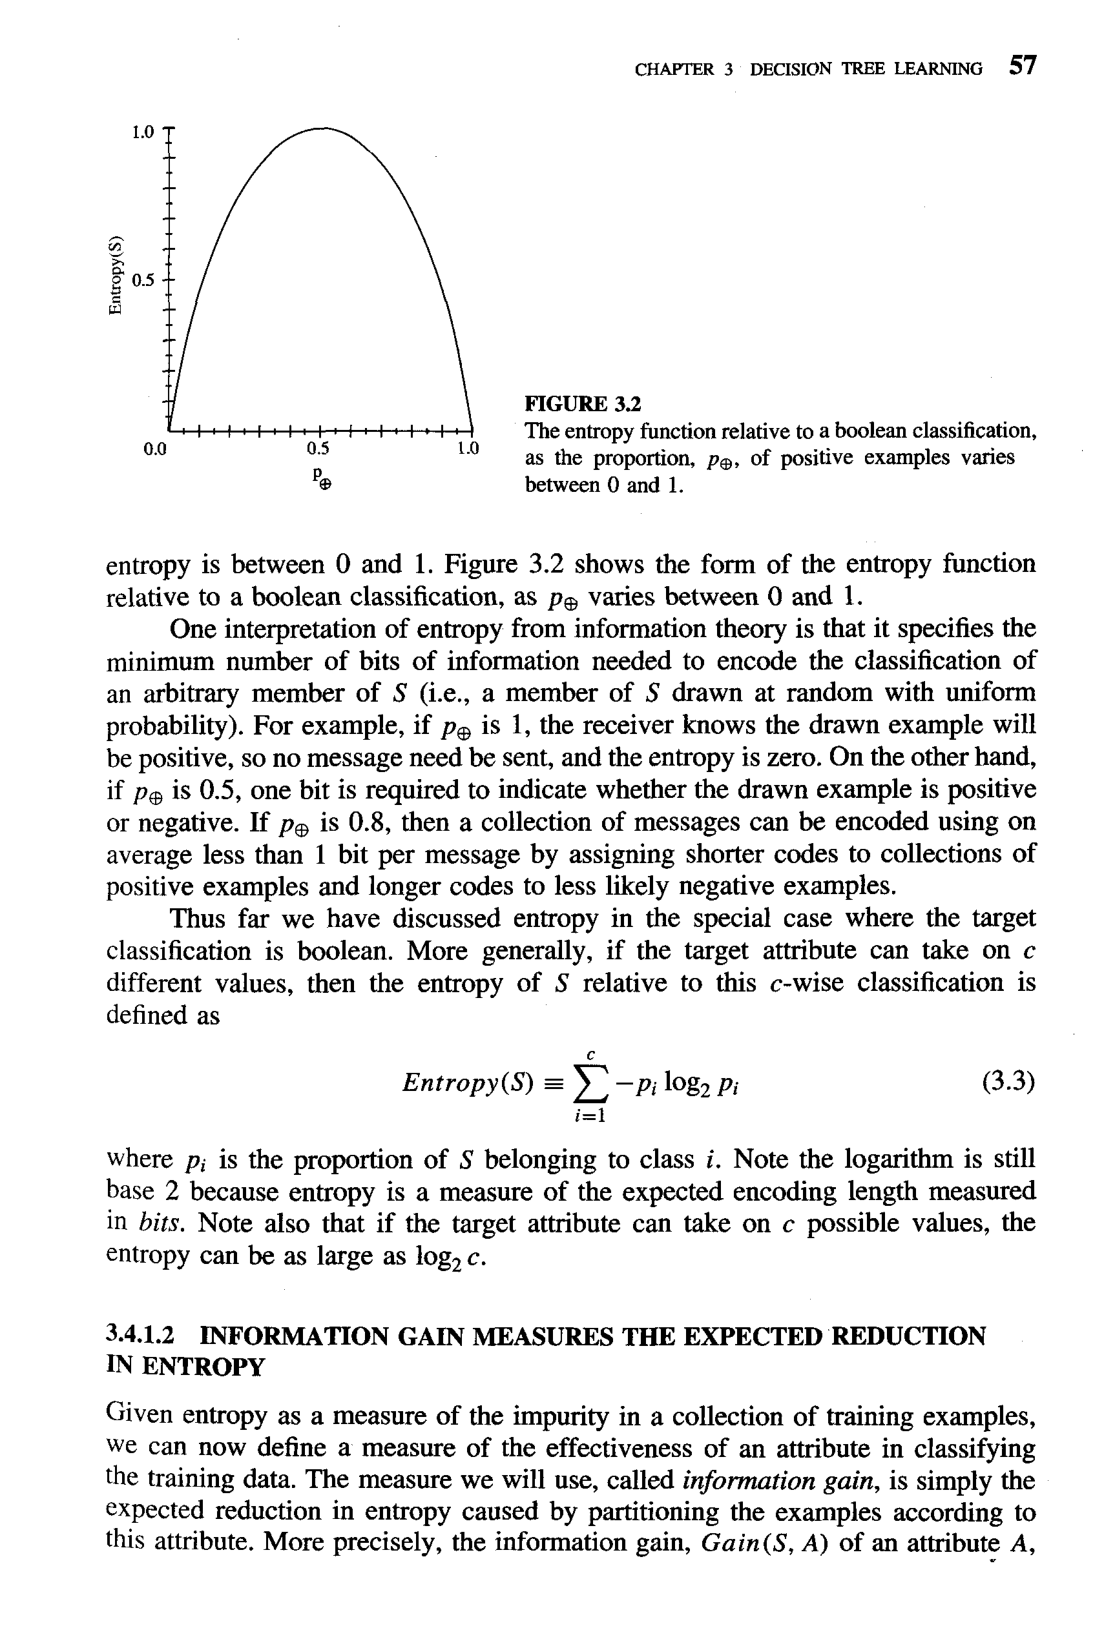
\includegraphics[width=0.9\linewidth]{figures/p69_b0.png}
\end{figure}

\subsection{CHAPTER 3 DECISION TREE LEARNING 57}

\noindent\textit{FIGURE 3.2 Hàm entropy liên quan đến classification boolean,}

\subsection{0,0 0,5 LO khi tỷ lệ pe của các mẫu dương thay đổi}

Pe giữa 0 và 1.

Entropy nằm trong khoảng từ 0 đến 1. Hình 3.2 cho thấy dạng của hàm entropy so với classification boolean, dưới dạng p, thay đổi trong khoảng từ 0 đến 1.

Một cách giải thích về entropy từ lý thuyết thông tin là nó chỉ rõ

Số bit thông tin tối thiểu cần thiết để mã hóa classification của một thành viên tùy ý của S (tức là một thành viên của S được rút ngẫu nhiên với xác suất đồng nhất). Ví dụ: nếu p, là 1, thì người nhận biết ví dụ được rút ra sẽ dương, do đó không cần gửi tin nhắn nào và entropy bằng 0. Mặt khác, nếu pe là 0,5 thì cần có một bit để cho biết ví dụ được vẽ là dương hay âm. Nếu pe là 0,8 thì một tập hợp các tin nhắn có thể được mã hóa với trung bình ít hơn 1 bit cho mỗi tin nhắn bằng cách gán mã ngắn hơn cho tập hợp các mẫu dương và mã dài hơn cho các mẫu âm ít có khả năng xảy ra hơn.

Cho đến nay chúng ta đã thảo luận về entropy trong trường hợp đặc biệt khi mục tiêu

Được phân loại là boolean. Tổng quát hơn, nếu thuộc tính đích có thể nhận c giá trị khác nhau thì entropy của S liên quan đến classification c-wise này được định nghĩa là

C

\subsection{Entropy(S) -pi log, pi}

\[i=l\]

Trong đó pi là tỷ lệ của S thuộc lớp i. Lưu ý logarit vẫn là cơ số 2 vì entropy là thước đo độ dài mã hóa dự kiến ​​được đo bằng bit. Cũng lưu ý rằng nếu thuộc tính đích có thể nhận c giá trị có thể thì entropy có thể lớn bằng log, c.

3.4.1.2 INFORMATION GAIN MEASURES THE EXPECTED REDUCTION IN ENTROPY

Cho entropy làm thước đo mức độ tạp chất trong tập hợp các ví dụ training, giờ đây chúng ta có thể định nghĩa thước đo về tính hiệu quả của một thuộc tính trong việc classification dữ liệu training. Biện pháp mà chúng ta sẽ sử dụng, được gọi là độ lợi thông tin, chỉ đơn giản là mức giảm entropy dự kiến ​​gây ra bởi việc phân vùng các ví dụ theo thuộc tính này. Chính xác hơn là mức tăng thông tin, Gain(S, A) của thuộc tính A,

% --- page 70 ---
\begin{figure}[ht]
\centering
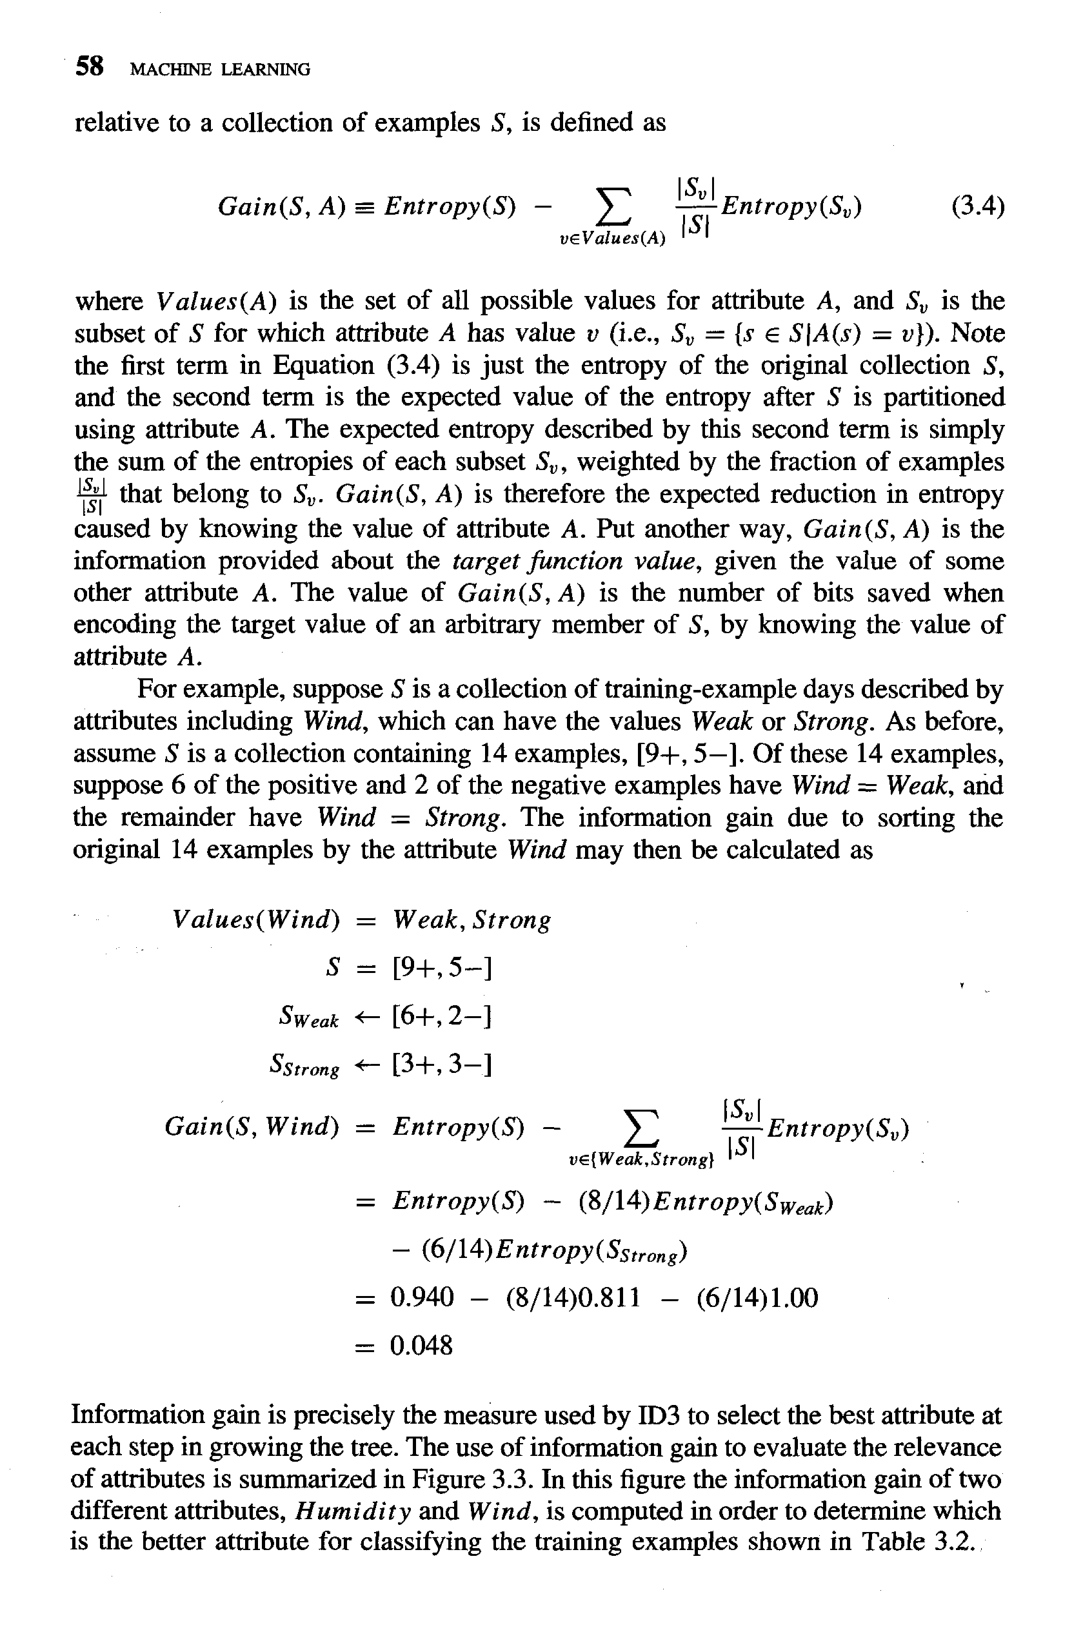
\includegraphics[width=0.9\linewidth]{figures/p70_b0.png}
\end{figure}

Liên quan đến tập hợp các ví dụ S, được định nghĩa là

\subsection{ISVl Tăng(S, A) I Entropy(S) -Entropy (S,)}

IS1 (3.4)

VeValues(A)

Trong đó Giá trị(A) là tập hợp tất cả các giá trị có thể có cho thuộc tính A và S là tập con của S mà thuộc tính A có giá trị v (tức là S, = \{s E SIA(s) = v)). Lưu ý số hạng đầu tiên trong phương trình (3.4) chỉ là entropy của tập hợp ban đầu S và số hạng thứ hai là giá trị kỳ vọng của entropy sau khi S được phân vùng bằng thuộc tính A. Entropy dự kiến ​​được mô tả bởi số hạng thứ hai này chỉ đơn giản là tổng các entropy của mỗi tập con S, được tính theo tỷ lệ của các ví dụ

Thuộc về S,. Gain(S, A) do đó là mức giảm entropy dự kiến

Gây ra bởi việc biết giá trị của thuộc tính A. Nói cách khác, Gain(S, A) là thông tin được cung cấp về giá trị đích \&hành động, cho giá trị của một số thuộc tính A khác. Giá trị của Gain(S, A) là số bit được lưu khi mã hóa giá trị đích của một thành viên tùy ý của S, bằng cách biết giá trị của thuộc tính A.

Ví dụ: giả sử S là tập hợp các ngày ví dụ training được mô tả bởi

Thuộc tính bao gồm Gió, có thể có giá trị Yếu hoặc Mạnh. Như trước, giả sử S là tập hợp chứa 14 ví dụ, [9+, 5-1. Trong 14 ví dụ này, giả sử 6 ví dụ tích cực và 2 ví dụ tiêu cực có Gió = Yếu, còn lại có Gió = Mạnh. Thông tin thu được nhờ sắp xếp 14 mẫu ban đầu theo thuộc tính Wind có thể được tính như sau:

\[Values(Wind) = Weak, Strong\]

\[IS, l Gain(S, Wind) = Entropy(S) -Entropy(S,)\]

\subsection{V\textasciitilde{}(Yếu,Mạnh] Is1}

Thu thập thông tin chính xác là thước đo được ID3 sử dụng để chọn thuộc tính tốt nhất ở mỗi bước trong quá trình phát triển cây. Việc sử dụng thông tin thu được để đánh giá mức độ liên quan của các thuộc tính được tóm tắt trong Hình 3.3. Trong hình này, mức tăng thông tin của hai thuộc tính khác nhau, Độ ẩm và Gió, được tính toán để xác định thuộc tính nào tốt hơn để classification các ví dụ training được hiển thị trong Bảng 3.2.

